% \iffalse meta-comment
%
% Copyright (C) 2018--2023 by Xiangdong Zeng <xdzeng96@gmail.com>
%
% This work may be distributed and/or modified under the
% conditions of the LaTeX Project Public License, either
% version 1.3c of this license or (at your option) any later
% version. The latest version of this license is in:
%
%   http://www.latex-project.org/lppl.txt
%
% and version 1.3 or later is part of all distributions of
% LaTeX version 2005/12/01 or later.
%
% This work has the LPPL maintenance status `maintained'.
%
% The Current Maintainer of this work is Xiangdong Zeng.
%
% \fi

%*********************************************************************
% fduthesis: 复旦大学论文模板
% 2023-05-27 v0.9a
%
% 重要提示:
%   1. 请确保使用 UTF-8 编码保存
%   2. 请使用 XeLaTeX 或 LuaLaTeX 编译
%   3. 请仔细阅读用户文档
%   4. 修改、使用、发布本文档请务必遵循 LaTeX Project Public License
%   5. 不需要的注释可以尽情删除
%*********************************************************************

\documentclass[type=master]{fduthesis}
% 模板选项:
%   type = doctor|master|bachelor  论文类型,默认为本科论文
%   oneside|twoside                论文的单双面模式,默认为 twoside
%   draft = true|false             是否开启草稿模式,默认关闭
% 带选项的用法示例:
%   \documentclass[oneside]{fduthesis}
%   \documentclass[twoside, draft=true]{fduthesis}
%   \documentclass[type=bachelor, twoside, draft=true]{fduthesis}

\fdusetup{
  % 参数设置
  % 允许采用两种方式设置选项:
  %   1. style/... = ...
  %   2. style = { ... = ... }
  % 注意事项:
  %   1. 不要出现空行
  %   2. “=” 两侧的空格会被忽略
  %   3. “/” 两侧的空格不会被忽略
  %   4. 请使用英文逗号 “,” 分隔选项
  %
  % style 类用于设置论文格式
  style = {
    % font = times,
    % 西文字体(包括数学字体)
    % 允许选项:
    %   font = garamond|libertinus|lm|palatino|times|times*|none
    %
    % cjk-font = fandol,
    % 中文字体
    % 允许选项:
    %   cjk-font = adobe|fandol|founder|mac|sinotype|sourcehan|windows|none
    %
    % 注意:
    %   1. 中文字体设置高度依赖于系统。各系统建议方案:
    %        windows:cjk-font = windows
    %        mac:    cjk-font = mac
    %        linux:  cjk-font = fandol(默认值)
    %   2. 除 fandol 和 sourcehan 外,其余字体均为商用字体,请注意版权问题
    %   3. 但 fandol 字体缺字比较严重,而 sourcehan 没有配备楷体和仿宋体
    %   4. 这里中西文字体设置均注释掉了,即使用默认设置:
    %        font     = times
    %        cjk-font = fandol
    %   5. 使用 font = none / cjk-font = none 关闭默认字体设置,需手动进行配置
    %
    % font-size = -4,
    % 字号
    % 允许选项:
    %   font-size = -4|5
    %
    % fullwidth-stop = catcode,
    % 是否把全角实心句点 “.” 作为默认的句号形状
    % 允许选项:
    %   fullwidth-stop = catcode|mapping|false
    % 说明:
    %   catcode   显式的 “。” 会被替换为 “.”(e.g. 不包括用宏定义保存的 “。”)
    %   mapping   所有的 “。” 会被替换为 “.”(使用 LuaLaTeX 编译则无效)
    %   false     不进行替换
    %
    footnote-style = xits,
    % 脚注编号样式
    % 允许选项:
    %   footnote-style = plain|libertinus|libertinus*|libertinus-sans|
    %                    pifont|pifont*|pifont-sans|pifont-sans*|
    %                    xits|xits-sans|xits-sans*
    % 默认与西文字体保持一致
    %
    % hyperlink = color,
    % 超链接样式
    % 允许选项:
    %   hyperlink = border|color|none
    %
    % hyperlink-color = default,
    % 超链接颜色
    % 允许选项:
    %   hyperlink-color = default|classic|material|graylevel|prl
    %
    bib-backend = bibtex,
    % 参考文献支持方式
    % 允许选项:
    %   bib-backend = bibtex|biblatex
    %
    % bib-style = numerical,
    % 参考文献样式
    % 允许选项:
    %   bib-style = author-year|numerical|<其他样式>
    % 说明:
    %   author-year  著者—出版年制
    %   numerical    顺序编码制
    %   <其他样式>   使用其他 .bst(bibtex)或 .bbx(biblatex)格式文件
    %
    % cite-style = {},
    % 引用样式
    % 默认为空,即与参考文献样式保持一致
    % 仅适用于 biblatex;如要填写,需保证相应的 .cbx 格式文件能被调用
    %
    bib-resource = {main.bib},
    % 参考文献数据源
    % 可以是单个文件,也可以是用英文逗号 “,” 隔开的一组文件
    % 如果使用 biblatex,则必须明确给出 .bib 后缀名
    %
    % logo = {fudan-name.pdf},
    % 封面中的校名图片
    % 模版已自带,通常不需要额外配置
    %
    % logo-size = {0.5\textwidth},      % 只设置宽度
    % logo-size = {{}, 3cm},            % 只设置高度
    % logo-size = {8cm, 3cm},           % 设置宽度和高度
    % 设置校名图片的大小
    % 通常不需要调整
    %
    % declaration-page = {declaration.pdf},
    % 插入扫描版的声明页 PDF 文档
    % 默认使用预定义的声明页,但不带签名
    %
    % auto-make-cover = true
    % 是否自动生成论文封面(封一)、指导小组成员名单(封二)和声明页(封三)
    % 除非特殊需要(e.g. 不要封面),否则不建议设为 false
  },
  %
  % info 类用于录入论文信息
  info = {
    title = {基于高维特征概率密度建模的模型不确定性的研究},
    % 中文标题
    % 长标题建议使用 “\\” 命令手动换行(不是指在源文件里输入回车符,当然
    % 源文件里适当的换行可以有助于代码清晰):
    %   title = {最高人民法院、最高人民检察院关于适用\\
    %            犯罪嫌疑人、被告人逃匿、死亡案件违法所得\\
    %            没收程序若干问题的规定},
    %
    title* = {Research on Model Uncertainty Based on High-Dimensional Feature Probability Density Modeling},
    % 英文标题
    %
    author = {师清},
    % 作者姓名
    %
    % author* = {Your name},
    % 作者姓名(英文 / 拼音)
    % 目前不需要填写
    %
    supervisor = {薛向阳\quad 教授},
    % 导师
    % 姓名与职称之间可以用 \quad 打印一个空格
    %
    major = {计算机技术},
    % 专业
    %
    degree = professional,
    % 学位类型
    % 允许选项:
    %   degree = academic|professional
    % 说明:
    %   academic      学术学位
    %   professional  专业学位
    %
    department = {计算机科学与技术},
    % 院系
    %
    student-id = {22210240262},
    % 作者学号
    %
    % date = {2023 年 1 月 1 日},
    % 日期
    % 注释掉表示使用编译日期
    %
    % secret-level = ii,
    % 密级
    % 允许选项:
    %   secret-level = none|i|ii|iii
    % 说明:
    %   none  不显示密级与保密年限
    %   i     秘密
    %   ii    机密
    %   iii   绝密
    %
    % secret-year = {五年},
    % 保密年限
    % secret-level = none 时该选项无效
    %
    instructors = {
      {薛向阳 \quad 教授},
      {戈维峰     \quad 青年副研究员}
    },
    % 指导小组成员
    % 使用英文逗号 “,” 分隔
    % 如有需要,可以用 \quad 手工对齐
    %
    keywords = {模型不确定性;高斯混合模型;梯度空间;输入扰动;特征空间;辅助损失函数},
    % 中文关键词
    % 使用英文逗号 “,” 分隔
    %
    keywords* = {Model Uncertainty; Gaussian Mixed Model;Gradient Space;Input perturbation;Feature Space;Auxiliary Loss Function},
    % 英文关键词
    % 使用英文逗号 “,” 分隔
    %
    % clc = {O413.1},
    % 中图分类号
    %
    % jel = {C02},
    % JEL 分类号,仅适用于经济学院等部分院系
  }
}

% 需要的宏包可以自行调用
\usepackage{physics}
\usepackage{algorithm}
%\usepackage{algorithmic}
%\usepackage{algorithmicx}
\usepackage{algpseudocode}
\usepackage{multirow}
\usepackage{makecell} % 使用 makecell 包
\usepackage{array}    % 用于表格的灵活控制
\newcolumntype{P}[1]{>{\centering\arraybackslash}p{#1}}
% 需要的命令可以自行定义
\newcommand{\hilbertH}{\symcal{H}}
\newcommand{\ee}{\symrm{e}}
\newcommand{\ii}{\symrm{i}}

\begin{document}

% 这个命令用来关闭版心底部强制对齐,可以减少不必要的 underfull \vbox 提示,但会影响排版效果
% \raggedbottom

% 前置部分包含目录、中英文摘要以及符号表等
\frontmatter

% 目录
\tableofcontents
% 插图目录
\listoffigures
% 表格目录
\listoftables

\begin{abstract}
近年来,深度学习在许多领域都有着广泛的应用,算法的准确率也在不断提高。但是在一些安全敏感的领域,如自动驾驶、医疗图像识别,即使模型以很低的概率预测错误,仍然会给应用带来严重的后果,极大限制了深度学习算法在这些领域的应用。于是就兴起了对神经网络不确定性的研究,神经网络的不确定性表示了神经网络对本次预测结果的信心,如果神经网络不确定性高,说明本次预测可靠程度低,通过选取一个阈值,对于不确定性高于某个阈值的预测,引入人类的判断,来降低线上系统事故发生的可能性。

对神经网络的建模有不同的思路,如贝叶斯神经网络(bnn),模型集成(Ensemble)的方法。本文采用的单一确定性神经网络建模不确定性的思路,通过对神经网络抽取的高维特征进行概率密度建模,并使用对数概率密度表示神经网络预测的模型不确定性。这种思路在DDU算法\cite{Mukhoti_2023_CVPR}中已经有了很好的效果,但是实验观察到相对于ensemble类的思路,DDU算法仍有差距,于是本文提出两点改进,提高了这一建模思路的效果。

首先是基于梯度空间的分析,对输入图片加上与梯度相关的扰动。通过可视化loss关于输入图片的梯度响应,观察到域内样本和域外样本存在明显的差异,域外样本的梯度较大,域内样本的梯度较小。对输入图片加入与梯度相关的输入扰动, 再用重新计算出的对数概率密度表示模型不确定性,通过在OOD检测任务,对抗样本检测任务上的实验,观察到方法对于模型不确定性建模的提升。

第二点改进是使用TSNE对高维特征降维到二维空间,然后对高维特征进行可视化分析,在此基础上本文指出通过提高特征空间的类内紧密性和类间可分性,可以进一步提高高维特征概率密度建模不确定性的效果,为了达到提高特征空间的类内紧密性和类间可分性这一目的,本文实验了几种辅助损失函数,和交叉熵损失函数一起联合训练神经网络模型,最终提出使用FeatureLoss,

总之,本文提出两个方法,改进了高维特征概率密度建模不确定性的效果,推进了深度学习算法在某些安全敏感领域的应用。
\end{abstract}

\begin{abstract*}
In recent years, deep learning has found extensive applications across various fields, achieving continually improving accuracy in its algorithms. However, in safety-critical domains such as autonomous driving and medical image recognition, even low-probability prediction errors can result in severe consequences, significantly limiting the application of deep learning algorithms in these areas. This challenge has led to a growing interest in studying the uncertainty of neural networks. Neural network uncertainty quantifies the confidence a network has in its predictions. High uncertainty implies low reliability of a prediction, and by setting a threshold, predictions with uncertainty above this threshold can be flagged for human review, thereby reducing the risk of accidents in online systems.

There are various approaches to modeling neural network uncertainty, such as Bayesian Neural Networks (BNNs) and ensemble methods. This paper adopts an approach based on a single deterministic neural network to model uncertainty. It models the probability density of high-dimensional features extracted by the network and uses the log-probability density to represent the uncertainty of predictions. This approach has demonstrated promising results in the DDU algorithm \cite{Mukhoti_2023_CVPR}, but experiments reveal that it still lags behind ensemble-based methods. To address this gap, this paper proposes two improvements to enhance the effectiveness of this modeling approach.

The first improvement involves gradient-space analysis by introducing gradient-related perturbations to the input images. By visualizing the loss gradient responses concerning the input images, it was observed that there are significant differences between in-domain and out-of-domain samples: the gradients for out-of-domain samples are generally larger, while those for in-domain samples are smaller. By adding gradient-related perturbations to the input images and recalculating the log-probability density to represent model uncertainty, experiments on OOD detection and adversarial sample detection tasks demonstrated improved modeling of model uncertainty.

The second improvement leverages t-SNE to reduce high-dimensional features to a two-dimensional space for visualization. Based on this analysis, the paper highlights that improving intra-class compactness and inter-class separability in the feature space can further enhance the effectiveness of probability density modeling for uncertainty. To achieve this, various auxiliary loss functions were experimented with and combined with the cross-entropy loss function to jointly train the neural network model. Ultimately, the paper proposes the use of FeatureLoss.

In conclusion, this paper introduces two methods to improve the effectiveness of high-dimensional feature probability density modeling for uncertainty, advancing the application of deep learning algorithms in safety-critical domains.
\end{abstract*}

% 符号表
% 语法与 LaTeX 表格一致:列用 & 区分,行用 \\ 区分
% 如需修改格式,可以使用可选参数:
%   \begin{notation}[ll]
%     $x$ & 坐标 \\
%     $p$ & 动量
%   \end{notation}
% 可选参数与 LaTeX 标准表格的列格式说明语法一致
% 这里的 “ll” 表示两列均为自动宽度,并且左对齐
\begin{notation}[ll]
  $D$                  & 数据集        \\

\end{notation}

% 主体部分是论文的核心
\mainmatter

% 建议采用多文件编译的方式
% 比较好的做法是把每一章放进一个单独的 tex 文件里,并在这里用 \include 导入,例如
%   \include{chapter1}
%   \include{chapter2}
%   \include{chapter3}

\chapter{绪论}
\section{研究背景和意义}
近年来随着计算机硬件的快速发展和数据的爆炸性增长,深度学习算法研究取得了显著进展,在图像识别\cite{krizhevsky2012imagenet}、自然语言处理\cite{brown2020language}、自动驾驶\cite{teichmann2018multinet}、医疗诊断\cite{gulshan2016development}等领域取得了广泛的应用。现阶段的深度学习算法在准确性上已经可以达到很好的效果,但仍普遍存在过度自信问题(Overconfident issue),即深度神经网络在其预测结果上往往过于自信,即使在它不熟悉的输入上,也可能错误地给出过高的预测概率。在一些高风险的领域,比如医疗诊断,自动驾驶等,错误的预测可能会带来严重的线上事故,这使得神经网络在这些领域的应用仍然受到限制。因此,在实际应用中,不仅需要模型能准确给出预测结果,还希望模型能给出一个值指示本次预测结果可靠程度,这就是神经网络的\textbf{不确定性(Uncertainty)}。神经网络预测结果的不确定性较高,就可以在必要时引入人类监督或放弃高风险决策,规避风险和灾难性后果。

对神经网络不确定性的相关研究具有重大意义。在实际应用中,对神经网络不确定性的研究有助于提升模型的鲁棒性,帮助模型更稳健、更可靠地应用于医疗、自动驾驶、金融等具体领域。不确定性量化(Uncertainty Quantification,UQ)可以帮助模型识别出对某些输入的预测信心不足的情况,避免错误决策引发的系统事故。

神经网络不确定性的研究对神经网络的可解释性也有重要意义,通过对神经网络不确定性的研究,学术界和工业界能够更深入地理解神经网络的行为和特性。当前多数研究和应用都把神经网络作为“黑箱”模型,其缺乏可解释性和透明性的问题长期以来阻碍了其在医疗、自动驾驶等安全关键领域的应用\cite{ROY201911}\cite{christoph2020interpretable}。通过不确定性研究,模型可以对自己的预测进行自我评价,为用户提供更直观的信心指标。这不仅有助于用户更好地理解和使用神经网络系统,还能增加对人工智能技术的信任。

最后,对神经网络不确定的研究也推动了深度学习理论的发展。当前,有关神经网络不确定性的研究已经催生了许多新的方法,例如深度高斯过程、贝叶斯神经网络、蒙特卡罗随机失活(MC dropout)、对抗训练等。这些方法不仅拓展了神经网络的理论基础,也为其他机器学习问题(如模型选择、主动学习、强化学习)提供了新的解决思路。



\section{不确定性的来源与分类}
\textbf{神经网络不确定性(Uncertainty in Neural Networks)}是指在神经网络的预测中,描述其对预测结果的置信程度\cite{abdar2021review}。神经网络的不确定性量化在许多实际应用中非常重要,尤其是在需要高可靠性和安全性的领域,如自动驾驶、医疗诊断和金融预测\cite{gawlikowski2023survey}\cite{he2023survey}\cite{gal2016uncertainty}。在实际应用中,神经网络中的不确定性通常可以分为两类\cite{abdar2021review}:\textbf{模型不确定性}(Model Uncertainty)和\textbf{ 数据不确定性}(Data Uncertainty)。

\textbf{模型不确定性},又称为\textbf{认知不确定性}(Epistemic Uncertainty),表示所训练的神经网络模型本身能力的局限性,模型不确定性可能来源于模型结构,训练过程,训练数据不足。当训练数据不足时,模型的参数未能很好地捕捉数据分布分布,导致预测的结果含有很大的模型不确定性。模型不确定性可以通过改变训练模型,优化训练过程,增加训练数据来减少。如图\ref{fig:uncertainty},在训练数据以外所呈现的高不确定性是模型不确定性。\textbf{数据不确定性}(Data Uncertainty), 又称为\textbf{偶然不确定性}(Aleatoric Uncertainty),通常是由数据本身的随机性或噪声引起,可能来源于数据收集时潜在的噪声或者数据标注时的错误。数据不确定性无法通过任务方式被消除。如图\ref{fig:uncertainty},种间训练数据本身所存在的误差和噪声引起的不确定性是数据不确定性。

\begin{figure}[H]
    \centering
    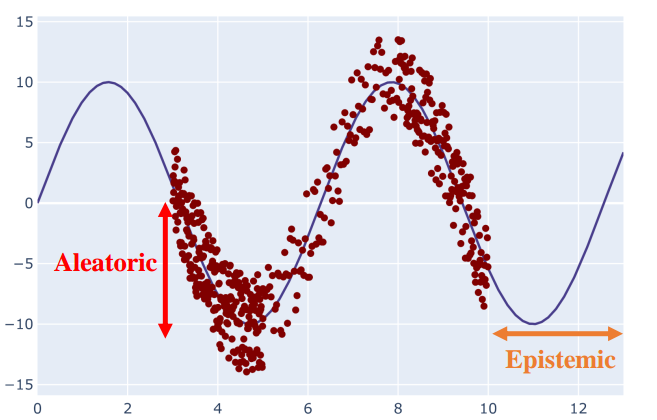
\includegraphics[width=0.9\linewidth]{assets/1-1.png}
    \caption{不确定性的来源与分类\cite{abdar2021review}
}
    \label{fig:uncertainty}
\end{figure}

数据不确定性和模型不确定性并非绝对的,可能会随着问题的定义有所变化\cite{hullermeier2021aleatoric}。Valdenegro-Toro等人\cite{valdenegro2022deeper}也在研究中发现,在解耦不确定性的过程中,模型不确定性和数据不确定性会相互影响,这一点是出乎意料的,因为通常认为只有模型不确定性应该与模型交互,而数据不确定性则不应和模型有关。



\section{不确定性研究的应用}
神经网络的不确定性研究(Uncertainty in Neural Networks)在许多应用场景中都具有重要价值,特别是在需要对预测结果的可靠性、稳定性和信心进行量化的任务中。传统的神经网络通常给出一个确定的预测结果(例如,分类标签或回归值),但并没有提供关于该结果的不确定性信息。而不确定性建模则能够量化模型对其预测的信心程度,这在多个领域中具有广泛的应用,以下简单介绍不确定性研究在自动驾驶、医疗诊断、金融、自然语言处理等领域的应用。

\textbf{1. 自动驾驶}

在自动驾驶系统中,车辆必须能够基于摄像头图像、雷达、激光雷达等数据预测和识别路况,并做出实时决策。然而,这些数据本身可能存在噪声,或者在复杂环境中不完全可靠。通过不确定性建模,自动驾驶系统可以识别哪些预测是可靠的,哪些可能需要进一步验证或修正。决策制定时结合不确定性,可以优先选择对结果不确定性较低的路径规划或行动,对不确定性较高的引入人工干预。近年来关于神经网络不确定性和自动驾驶领域的结合出现很多研究,Di Feng, Lars Rosenbaum等人\cite{feng2018towards}针对激光雷达(LiDAR)的3D车辆检测任务,提出了一种结合贝叶斯深度学习的方法,能够同时估计数据不确定性和模型不确定性,通过不确定性信息优化预测结果,增强了自动驾驶系统在复杂环境中的安全性和稳健性。Hujie Pan等人\cite{pan2020towards}针对激光雷达(LiDAR)的3D车辆检测任务,结合不确定性估计方法,对回归的坐标引入拉普拉斯分布,设计了一种改进的损失函数,获得了更具有解释性和可靠性的预测结果。SalsaNext\cite{cortinhal2020salsanext} 是一种针对自动驾驶领域设计的高效、不确定性感知的语义分割模型,用于处理 LiDAR 点云数据。它在原有 SalsaNet\cite{Aksoy2019SalsaNetFR}的基础上进行了改进,结合了注意力机制和贝叶斯学习框架,实现了更高的精度和不确定性估计能力,为自动驾驶中的环境感知提供了可靠的解决方案。赵洋\cite{QCYK202405002}深入研究了自动驾驶领域目标检测任务上的不确定性估计的方法,利用不确定性信息来提高目标检测的准确性,并总结了不确定性估计的评价指标。

\textbf{2. 医疗诊断}

在智能辅助诊断领域,尤其是在面对复杂或模糊的医学影像时,对不确定的研究能够为医生提供关于某项影像诊断的置信度,帮助医生判断是否需要进一步的检查或其他医学手段。在疾病预测方向上,基于患者历史数据和医学影像,模型预测某种疾病的风险,并通过不确定性量化本次预测的可信度,对不确定度高的预测引入专业医生的判断,可以减少误诊率,降低医疗事故的可能性。在医学图像检测或者分割任务中,某些图像可能很模糊,此时模型不仅需要做出准确的预测,还需要能够提供关于其预测结果不确定性的估计,通过不确定性估计,模型可以指出分割结果的可靠区域,辅助医生进行更准确的解读。不确定性在医疗诊断领域应用上的研究,Guotai Wang等人\cite{wang2019aleatoric}研究如何结合测试时增强的方法,对卷积神经网络进行不确定性估计,从而提高医学图像分割的鲁棒性。Tanya Nair等人\cite{nair2020exploring}针对病变检测和分割,提出了一种改进的U-Net架构,结合了四种不确定性度量:预测方差、蒙特卡罗样本方差、预测熵和互信息,辅助识别模型在预测中的不确定区域,提高病变分割的准确性。邹可\cite{1024642336.nh}使用证据网络进行不确定性估计方法的研究,将不确定性估计应用到医学分割领域,提高了医学图像分割的准确性和可靠性。


\textbf{3. 金融风控与预测}

在金融行业中,不确定性量化有助于提高风险管理和预测系统的可靠性,尤其是在面对市场波动和不确定环境时。在信贷风险评估上,通过不确定性量化,金融机构能够识别贷款申请中哪些因素对违约预测有较高不确定性,从而采取更谨慎的风险管理措施。在市场预测上,量化市场趋势预测中的不确定性,可以帮助投资者做出更明智的决策,尤其在市场波动较大的情况下。在金融行业中,关于不确定性的研究,WONG SY等人\cite{wong2025quantifying}研究了不确定性量化对复杂金融时间序列预测的必要性,聚焦于时间序列中的波动性聚集特性(如资产回报率预测),提出了一种结合模型集成和证据网络的方法,显著提高了金融市场中加密货币和股票的预测的不确定性量化效果。

\textbf{4. 自然语言处理}

在自然语言处理任务中,神经网络通常需要处理复杂的文本和语言,不仅要生成准确的输出,还要提供预测的不确定性。例如,在机器翻译、情感分析或问答系统中,了解模型对预测结果的置信度对于理解其输出的可信度非常重要。在机器翻译领域,模型可以提供翻译的置信水平,帮助用户理解哪些翻译结果可靠,哪些可能需要进一步验证。在情感分析领域,评估情感分析模型的预测可信度,帮助商家了解用户评论中的潜在情感。在自动问答系统中,不确定性建模可以提供关于某个答案的置信度,帮助系统在遇到不确定的答案时请求进一步的信息或向用户确认。在自然语言处理领域关于不确定性的研究,郭晓亭\cite{1022812574.nh} 设计了一种不确定性感知的损失函数,提高了文本情感分析准确性。X. Han等人\cite{han2019attention} 提出一个基于注意力机制的神经网络框架,识别社交媒体文本中的不确定性。近年来大语言模型的兴起和广泛应用,也催生了关于不确定性在大模型方向上的研究。Lorenz Kuhn等人\cite{kuhn2023semantic}介绍了一种用于衡量大语言模型不确定性的方法,对于像问答任务这样的应用,作者提出了“语义熵”概念,通过广泛的消融实验,作者证明了语义熵在问答数据集上的表现优于其他对比基准,能够更有效地预测模型的准确性。Zhen Lin\cite{lin2024generating}针对大型语言模型(LLMs)在自然语言生成任务,特别是在黑箱模型的场景下,提出了多种不确定性量化指标,筛选不可靠的结果或将其交由人工进一步评估。

% 5. 机器人与自主系统

% 深度学习在机器人领域面临独特挑战,例如测试条件与训练分布不一致可能导致性能下降。因此,研究如何量化神经网络预测的不确定性,以避免灾难性错误,对于推动机器人技术的发展尤为重要。在路径规划与控制方面,通过不确定性量化,机器人可以识别哪些路径或动作是更安全的,哪些决策可能会导致更高的风险。在环境感知方向上,在复杂环境中(例如多变的室内环境或户外环境),机器人可以基于不确定性评估来选择更可靠的传感器数据进行决策。有关不确定性量化在机器人方向上的研究,Peretroukhin, Valentin and Giamou\cite{peretroukhin2020smooth}引入了一种概率分布表示,将旋转表示和不确定性建模相结合,可以更准确地学习旋转,同时提供对模型置信度的估计,从而在姿态估计和物体跟踪任务中表现更出色。。Yang等人\cite{yang2020d3vo}的研究通过联合学习场景深度、相机位姿以及不确定性估计,构建了一个端到端的框架,通过引入不确定性评估以增强对环境变化的适应性。


\section{问题定义和研究内容}
目前,关于模型不确定性的研究已经提出了多种方法,常见的技术包括贝叶斯神经网络、模型集成以及单一确定性网络建模等。每种方法在计算复杂性、存储开销和不确定性建模效果方面各不相同。贝叶斯神经网络通过为神经网络的权重分配概率分布,从而在推理过程中显式地建模模型的不确定性。其优点在于能够精确地建模模型的不确定性,并具有坚实的理论基础;缺点是训练过程较为缓慢,且计算和存储开销较大。模型集成方法通过训练多个模型并将其预测结果进行结合,从而获得预测的不确定性。集成方法优点是能够通过多个模型的结合,更好地捕捉数据的多样性,从而增强不确定性的建模能力;缺点是计算和存储成本较高,随着集成模型数量的增加,计算复杂度将迅速上升。

与贝叶斯神经网络和模型集成方法相比,单一确定性网络建模方法具有较低的计算成本。在这种方法中神经网络采用确定性架构,权重为固定值,不进行概率分布建模。为了量化不确定性,单一确定性建模方法可以通过对高维特征的概率密度估计来计算不确定性。具体而言,网络可以在训练集上学习到的高维特征进行概率分布估计,而在测试时,输入数据提取的特征将与该分布对比,从而量化预测的不确定性。相较于贝叶斯神经网络和模型集成方法,单一确定性建模方法的优点是计算和存储成本较低,避免了多次推理或训练多个模型的开销,且训练过程较为简便,然而,该方法在不确定性建模的效果上仍存在一定不足。

为更高效地建模神经网络的不确定性,本文进一步研究基于高维特征概率密度估计的模型不确定性量化方法。该方法在DDU算法\cite{Mukhoti_2023_CVPR}中已被提出并进行初步研究。尽管该算法在不确定性建模方面取得了一定进展,实验结果表明,与当前最优的模型集成方法相比,DDU算法仍存在一定差距。因此,本文的核心研究问题是:为了更高效准确地建模神经网络的不确定性,在DDU算法的基础上,进一步探索并改进基于高维特征概率密度估计的不确定性建模方法,以提升不确定性建模效果,并在域外样本检测、对抗样本识别和主动学习等任务中验证所提出改进方法的有效性。

本文的研究内容主要包括两个方面。其一,本文研究了对一个已经训练好的网络,在不重新改变训练方式的前提下,如何提高基于高维特征概率密度估计的模型不确定性的建模效果。本文通过计算输出对输入图片的梯度并绘制梯度响应图,实验观察到分布外样本和分布内训练样本的梯度分布存在显著差异,分布外样本的梯度响应显著更大。基于这一发现,本文提出将梯度相关的信息作为扰动引入到输入图片中,并重新计算其概率密度。同时,通过推导和理论分析,证明了加入梯度相关扰动能够有效拉大分布内样本和分布外样本的分布差距,从而提升不确定性建模的效果。通过在OOD检测、对抗样本识别和主动学习等任务上的实验评估,结果表明加入输入扰动可以显著提升基于高维特征概率密度建模的不确定性效果。

其二,本文研究如何通过改进训练方式,提高基于高维特征概率密度估计的模型不确定性建模效果。本文通过对神经网络提取的特征空间进行分析并指出,提升特征空间的类内紧密性和类间可分性能够显著改善基于高维特征概率密度估计的不确定性建模效果。基于度量学习的思想,本文设计了一种全新的辅助损失函数,并将其与交叉熵损失函数结合进行联合训练。在联合训练后的特征空间上建模概率分布,并使用概率密度量化模型不确定性。通过对联合训练后的特征空间进行定量分析,结果表明联合训练显著提升了类内紧密性和类间可分性。在OOD检测、误分类样本识别等任务中的评估结果进一步验证了联合训练方法能够有效提升基于高维特征概率密度的不确定性建模性能。此外,为解决高维特征导致的存储复杂度问题,本文还提出使用主成分分析对高维特征进行降维。在降维后的特征空间上进行概率分布建模不仅能够显著降低存储需求,同时还提高了建模效果。理论与实验均证明了这一策略的有效性。


本文的研究内容与创新点总结如下:
\begin{itemize}
    \item 提出概率密度关于输入的梯度在分布内样本和分布外样本之间存在显著差异,并通过推导和理论分析进行解释。
    \item 提出针对输入图片添加梯度相关扰动的方法,能够拉大分布内样本和分布外样本的分布差距,从而提升不确定性建模效果。
    \item 基于度量学习思想,设计一种新的辅助损失函数,与交叉熵损失函数联合训练,以优化特征空间的类内紧密性和类间可分性。
    \item 使用主成分分析对高维特征降维,显著降低存储复杂度,提升建模效率与效果。
\end{itemize}



\section{章节安排}
本文共分五章内容组织。

第一章主要是对不确定性的介绍,介绍了不确定性研究的背景和意义,不确定性的定义、来源与分类,不确定性研究的相关应用。

第二章介绍了关于不确定性的一些理论知识。首先介绍当前主流的建模不确定性的思路,主要包括贝叶斯神经网络,模型集成,测试数据增强,单一确定性网络建模的方法,并介绍了这些方法是如何计算不确定性的。由于在实际场景中缺乏不确定的标注,所以直接评估不确定性建模效果是很困难的,在第二章最后介绍是如何通过OOD检测、误分类样本识别、主动学习等代理任务间接评估不确定性的建模效果。

第三章主要介绍了基于输入扰动的改进策略,首先基于对梯度空间的分析,本章指出分布外样本和分布内样本的梯度分布存在显著差异,分布外样本的梯度响应显著更大,之后通过理论分析证明这一结论。基于此,在这一章提出将梯度相关的信息作为扰动引入到输入图片中,加入梯度相关扰动能够有效拉大分布内样本和分布外样本的分布差距,最后在OOD检测、误分类样本识别等代理任务上验证了改进后的方法对不确定性的建模效果的提升。

第四章主要介绍了使用辅助损失函数联合训练的改进,首先是对特征空间的分析,指出提升特征空间的类内紧密性和类间可分性能够显著改善高维特征概率密度建模的不确定性效果,进而提出一个新的辅助损失函数和交叉熵损失函数一起联合训练,为了减少模型存储还提出了对高维特征使用主成分分析降维,最后在OOD检测等任务上评估了改进后的方法的建模效果。

第五章是对本文研究的总结和对神经网络不确定性研究的未来的展望。

\chapter{相关工作与理论}
\section{引言}
本章从不确定性的建模方法,不确定性的计算,不确定性建模方法的评估等三个角度介绍不确定性的相关理论和研究工作。最近几年关于不确定性的建模方法兴起了许多不同的思路,从单个神经网络建模到集成多个模型建模,从神经网络权重参数确定到神经网络权重参数符合某个分布。关于神经网络的不确定性的计算,是指给定某种建模思路,如何计算出一个标量表示不确定性。一些计算方法把神经网络的数据不确定性和模型不确定性分开,一些方法则不分开。由于大多数情况下,神经网络的不确定性是缺乏标签信息的,所以没办法直接评估一种建模思路计算出的不确定性的好坏,只能通过一些代理任务上的表现,来间接地反映建模方法的好坏。下面从这三个方面依次论述。

\section{不确定性的建模方法}
目前,在神经网络不确定性的研究上,提出了许多建模方法:
\begin{itemize}
    \item 贝叶斯神经网络:通过在神经网络中引入贝叶斯推断,建模权重参数的不确定性,从而获得模型的输出不确定性。
    \item Ensemble的方法:通过训练多个神经网络,对于同一个输入,可以得到多个预测结果,进而通过计算多个预测值的方差或者熵来建模不确定性
    \item Test Time Augmentation的方法:通过对输入做数据增强,得到多个增强后的输入,然后进入训练好的神经网络中预测多次得到多个预测结果,进而计算模型输出的不确定性。
    \item 单一确定的神经网络来建模不确定性:这类方法使用单一确定性的神经网络建模不确定性
\end{itemize}

\subsection{贝叶斯神经网络}
贝叶斯神经网络是一种将贝叶斯统计方法与深度学习相结合的模型,通过对神经网络的参数引入概率分布,量化模型的不确定性。 在传统神经网络中,参数(权重和偏置)是固定值;而在贝叶斯神经网络中,如图2-1,参数被视为随机变量,遵循某种概率分布(如高斯分布)。这种方法使模型输出不仅仅是一个确定值,而是一个分布,从而反映模型的置信程度。贝叶斯神经网络加建模不确定性的基本思路如下。

\begin{figure}[H]
    \centering
    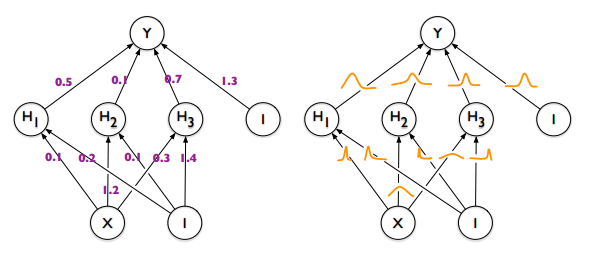
\includegraphics[width=0.75\linewidth]{assets/2-1.png}
    \caption{贝叶斯神经网络\cite{blundell2015weight}
}
    \label{fig:enter-label}
\end{figure}


\begin{itemize}
    \item \textbf{贝叶斯推断}:
    通过贝叶斯公式来求解参数分布:
    \[
    P(\theta \mid \mathcal{D}) = \frac{P(\mathcal{D} \mid \theta) P(\theta)}{P(\mathcal{D})}
    \]
    其中:
    \begin{itemize}
        \item \( P(\theta \mid \mathcal{D}) \):后验分布(目标分布)。
        \item \( P(\mathcal{D} \mid \theta) \):似然函数(数据生成概率)。
        \item \( P(\theta) \):先验分布(参数的初始假设)。
        \item \( P(\mathcal{D}) \):边际似然,用于归一化。
    \end{itemize}
    
    \item \textbf{输出分布}:
    当输入图片到贝叶斯神经网络里预测时,输出的不是单一值,而是一个分布。从关于参数的后验分\( P(\theta \mid \mathcal{D}) \)采样多个 \( \theta \),通过这些 \( \theta \) 计算多个 \( y \),对 \( y \) 进行汇总(如计算熵或方差)得到不确定性。
\end{itemize}

贝叶斯神经网络的难题是后验分布 \( P(\theta \mid \mathcal{D}) \) 的估计。由于直接计算后验分布 \( P(\theta \mid \mathcal{D}) \) 通常是不可行的,贝叶斯神经网络采用近似方法,通常的近似手段有采样(如马尔科夫链蒙特卡罗方法),变分推断,拉普拉斯近似等几种。马尔科夫链蒙特卡罗(MCMC)方法是一种通过随机抽样来逼近后验分布的方法。常见的 MCMC 算法包括 Metropolis-Hastings 算法和 Gibbs 采样。它们通过生成一系列样本来估计后验分布,但计算开销较大,尤其是在高维参数空间中。变分推断通过将后验分布近似为一个简单的分布族(例如高斯分布)来进行推断。它通过最小化某种距离度量(如 Kullback-Leibler 散度)来优化参数,使得近似分布尽可能接近真实的后验分布。变分推断通常计算更高效,适用于大规模数据集。:拉普拉斯近似通过在后验分布的最大后验估计(MAP)附近用二次泰勒展开来近似后验分布。该方法对于参数空间较小或者后验分布接近高斯分布的情况特别有效。Charles Blundell\cite{blundell2015weight}等人提出了Bayes By Backprob算法高效第计算权重参数的后验分布。Yarin Gal\cite{gal2016dropout}等人提出了MC Dropout的方法来近似。这种方法在预测阶段保留 Dropout,并通过多次前向传播获得样本分布,是一种近似贝叶斯推断的实用方法。 Hippolyt Ritter\cite{ritter2018scalable}等人通过构建  Kronecker分解的拉普拉斯近似,近似求解权重参数的后验分布。Welling等人\cite{welling2011bayesian}提出了一种称为 Stochastic Gradient Langevin Dynamics (SGLD) 的方法,结合了随机梯度下降 (SGD) 和 Langevin 动力学的思想,用随机梯度近似后验分布,同时引入噪声来模仿MCMC采样过程。



\subsection{Ensemble的方法}
集成(Ensemble)方法\cite{lakshminarayanan2017simple}是一种通过结合多个模型的预测来提高性能和鲁棒性的技术。在建模不确定性时,集成方法的核心思想是通过多个独立模型的多样性来量化预测结果的可信度。以下是关于使用集成方法建模不确定性的详细说明。集成方法训练多个独立的模型,每个模型从不同的角度对数据进行学习。通过将这些模型的预测结果进行组合(例如取平均),可以提高整体的预测性能并提供不确定性估计。以下是Ensemble类方法的建模步骤:


\begin{enumerate}
    \item \textbf{训练多个模型}:
    训练 \( M \) 个独立的神经网络模型 \( f_1(x), f_2(x), \ldots, f_M(x) \),其中每个模型的参数初始化不同,或者使用不同的训练数据子集(如 Bagging 方法)。

    \item \textbf{预测分布}:
    对于给定输入 \( x \),每个模型生成一个预测 \( y_i = f_i(x) \)。集成方法的预测分布可以通过这些独立模型的输出构造, 通过汇总预测分布的统计量(如方差、熵)来评估不确定性。
    \[
    P(y \mid x) \approx \frac{1}{M} \sum_{i=1}^M P(y \mid f_i(x))
    \]
\end{enumerate}

Y Wen\cite{wen2020batchensemble}等人提出BatchEnsemble解决Ensemble方法需要训练多个模型的存储和计算复杂度,BatchEnsemble 将一个大模型分解为多个小模型,每个小模型具有自己的参数化方式,但它们共享同一个主干模型的参数。通过共享基础权重 W,BatchEnsemble 避免了传统ensemble方法中每个模型都需要独立存储全部参数的缺点。BatchEnsemble 大大减少了内存占用和计算需求。




\subsection{Test Time Augmentation的方法}
Test Time Agmentation(测试时数据增强,TTA)的方法是一种通过对测试数据应用多种数据增强方式来估计模型预测不确定性的方法。该方法通过将同一输入的不同增强版本的预测结果进行汇总,量化模型对该输入的置信程度。


\begin{enumerate}
    \item \textbf{数据增强}:
    对测试数据 \( x \),应用一系列数据增强操作 \( T_1, T_2, \ldots, T_N \),生成多个增强版本 \( \{ T_i(x) \}_{i=1}^N \)。

    \item \textbf{预测分布}:
    对每个增强版本,模型 \( f \) 生成对应的预测结果 \( \{ f(T_i(x)) \}_{i=1}^N \)。这些预测结果的分布可以反映模型的不确定性。
    通过汇总预测分布的统计量(如方差、熵)来评估不确定性。
\end{enumerate}

在TTA的建模方法中,一个重要的问题是如何选择有效的数据增强方式。Divya Shanmugam等人\cite{shanmugam2020and}探讨了如何选择合适的增强策略,以及在结果聚合(如简单平均、加权平均)中的设计方法。




\subsection{单一确定性神经网络建模}
还有很重要的一类建模不确定性的方法是使用单一确定性的网络进行建模。所谓单一确定神经网络,这里的单一是指只需要训练一个神经网络,不像Ensemble类方法需要训练多个网络;这里的确定是指网络参数是确定的,不像贝叶斯神经网络一样符合某个分布。这类方法建模不确定性通常直接从单一确定性模型的输出中直接推导出不确定性。这类方法通过模型结构或损失函数设计,使模型能够在不需要多模型或参数采样的情况下提供对不确定性的量化,从而降低计算和存储成本。单一确定神经网络可以分为Internal Methods和Externel Methods\cite{gawlikowski2023survey}。

Internal Methods是指不使用额外的头去预测不确定性,不确定性的计算和原有神经网络的预测是一起的。这类方法中,Prior Network\cite{malinin2018predictive} 通过引入一个显式的先验分布来对分类问题中的不确定性建模。这种方法使用一个神经网络直接对分类器的分布进行建模,而不是仅输出点估计。Prior Network 的输出是一个分类概率分布的参数,例如 Dirichlet 分布的参数$\alpha$,用以表征预测的不确定性。Murat Sensoy等人\cite{sensoy2018evidential}提出了一个新方法,通过引入主观逻辑理论,在神经网络的分类概率上使用狄利克雷分布来量化不确定性。该方法将神经网络的分类结果视为主观意见,网络学习如何根据数据收集证据来支持每个类别的预测。这种方法不仅能预测分类结果,还能量化预测的不确定性,从而提升模型的鲁棒性,特别是在面对对抗样本和分布外数据时。
深度核学习(Deep Kernel Learning)\cite{van2021feature}结合深度神经网络和高斯过程,将神经网络的输出作为核函数的输入,捕捉数据的不确定性。

Internal Methods中,一种经常作为不确定性领域Baseline的方法是使用最大预测概率\cite{hendrycks2017a}(Maximum Softmax Probability, MSP)作为不确定性的度量。作者观察到,OOD 样本的MSP值通常会低于inD样本。因此可以使用MSP来建模不确定性。当分类器遇到ID样本时,输出的类概率高 (置信度高) ,遇到OOD样本时,输出的概率虽然比较高。MSP优点是简单易实现,直接利用现有神经网络的 softmax 输出,无需修改网络架构或增加额外的训练开销。MSP 的计算仅需一次前向传播,非常适合实时场景。缺点是如果分布内数据和分布外数据在特征空间上高度重叠,MSP 的建模不确定性的能力可能不足。DUQ\cite{van2020uncertainty}通过使用与径向基函数(RBF)的结构,训练一个可以在推理时通过一次前向传播计算不确定性的模型。SNGP\cite{liu2020simple}核心思想是引入输入距离感知,即模型能够量化测试样本与训练数据之间的距离,从而准确评估预测的不确定性。为了实现这一点,论文提出了谱归一化神经高斯过程(SNGP),通过在训练中加入权重归一化步骤和替换倒数第二层的激活函数来增强模型的距离感知能力。
论文\cite{charpentier2023training}探讨了对于单一确定性的神经网络,不确定性的建模和神经网络架构和训练方式的关系。

Externel Methods显式地在原有模型基础上额外添加一个头来预测不确定性。Maithra Raghu等人\cite{raghu2019direct}提出了一种直接不确定性预测(Direct Uncertainty Prediction, DUP)方法,通过神经网络直接预测医学诊断任务中的预测置信度。由于不确定性标注的困难性,关于这类建模不确定性方法很少。


\subsection{以上主流方法的对比}
下面对比以上列举的四类建模不确定性方法的优缺点。

贝叶斯神经网络建模不确定性具有以下优点:1.良好的可解释性,有非常好的数学基础。2.通过对参数的概率建模,BNN天然具有正则化效果。3.在数据较少时,先验分布能提供有用的信息,提高模型的性能。4.对输入噪声或异常值有更高的鲁棒性。贝叶斯神经网络建模不确定性具有以下挑战和局限:1.参数分布的推断和采样导致计算复杂度远高于传统神经网络。2.随着网络规模的增加,推断过程可能变得难以处理。3.先验分布的选择对模型性能有重要影响,但通常难以确定。4.变分推断或 MCMC 方法训练困难,可能收敛缓慢,需要调整超参数。


基于Enseble建模不确定性的方法有以下优点:1.集成方法通过多模型组合降低单个模型的过拟合风险,提供更可靠的预测。2.集成方法不需要对现有模型结构进行修改,适合与各种神经网络架构结合。基于Enseble建模不确定性的方法有以下局限性:1.训练多个模型会显著增加计算资源需求,尤其是在深度学习场景中。2.每个模型都需要存储其独立的参数,这可能导致较高的存储需求。3.集成效果高度依赖于各个模型的多样性和质量。如果模型过于相似,集成方法的优势可能难以体现。

TTA建模不确定性的优点是:简单易实现,无需修改模型结构或训练过程,直接利用测试阶段的增强技术即可。TTA建模不确定性的缺点是:1.需要对同一输入进行多次推理,增加推理时间。2.不同的增强策略可能导致不确定性估计的效果差异,需要精心设计数据增强方式。


单一确定网络建模不确定性的方法具有以下优点:1.高效的建模方法,不需要多次采样或集成多个模型,推理速度快,计算成本低,高效。2.仅通过设计输出和损失函数即可实现,易于与现有的神经网络框架结合。单一确定网络建模不确定性的方法具有以下局限性:模型输出的分布假设(如高斯分布)可能无法充分建模复杂数据的分布,导致不确定性的建模效果不好。

\section{不确定性的计算方法}
针对不同的建模不确定性的方法,对不确定性的计算在各不相同。在分类任务上和回归任务上,对于不确定性的计算也不相同。有的关于不确定性的计算区分开模型不确定性和数据不确定性,有的则不分开,只计算总的预测不确定性。以下列举几种常见情况下不确定性的计算公式。

\subsection{分类任务中不确定性的计算}

\textbf{预测概率的不确定性}:对于每个分类任务,模型输出每个类别的预测概率。模型的不确定性可以通过评估这些预测概率的分布来衡量。常见的计算方法包括:最大概率法
    \[
    P_{\text{max}} = \max_{i} P(y_i | \mathbf{x})
    \]
    其中,\( P(y_i | \mathbf{x}) \) 是模型对样本 \( \mathbf{x} \) 的类别 \( y_i \) 的预测概率。最大概率 \( P_{\text{max}} \) 越接近1,表示模型的确定性越高;越接近0.5(对于二分类任务),表示不确定性较高。


\textbf{熵(Entropy)}:熵是衡量概率分布不确定性的标准方法。对于分类任务,熵的计算公式为:
\[
H(\mathbf{x}) = - \sum_{i=1}^{C} P(y_i | \mathbf{x}) \log P(y_i | \mathbf{x})
\]
其中,\( C \) 是类别数,\( P(y_i | \mathbf{x}) \) 是样本 \( \mathbf{x} \) 被预测为类别 \( y_i \) 的概率。熵越大,表示模型对样本的分类越不确定。

\textbf{方差(Variance)}:对于多个模型预测或多次模型预测,可以使用预测方差来衡量不确定性:
\[
\text{Var}(\mathbf{x}) = \frac{1}{T} \sum_{t=1}^{T} \left( P_t(y | \mathbf{x}) - \bar{P}(\mathbf{x}) \right)^2
\]
其中,\( T \) 是模型预测的次数,\( P_t(y | \mathbf{x}) \) 是第 \( t \) 次预测的概率,\( \bar{P}(\mathbf{x}) \) 是所有预测概率的平均值。

\textbf{互信息(Mutual Information)}:互信息衡量了输入特征与输出类别之间的信息共享量。在分类任务中,输入特征 \( \mathbf{x} \) 和输出类别 \( y \) 之间的互信息可以计算为:
\[
I(\mathbf{x}; y) = H(y) - H(y | \mathbf{x})
\]
其中,\( H(y) \) 是类别 \( y \) 的熵,表示输出的总体不确定性,\( H(y | \mathbf{x}) \) 是在给定输入 \( \mathbf{x} \) 的条件下,类别 \( y \) 的条件熵,表示输入特征给出的信息后,输出类别的剩余不确定性。互信息越大,表示输入特征与输出类别之间的关系越强,从而模型的预测不确定性越小。

互信息也可以用联合概率分布表示:
\[
I(\mathbf{x}; y) = \sum_{i=1}^{C} \sum_{j=1}^{N} P(y_i, \mathbf{x}_j) \log \frac{P(y_i, \mathbf{x}_j)}{P(y_i) P(\mathbf{x}_j)}
\]
其中,\( P(y_i, \mathbf{x}_j) \) 是类别 \( y_i \) 和输入特征 \( \mathbf{x}_j \) 的联合概率分布,\( P(y_i) \) 和 \( P(\mathbf{x}_j) \) 分别是类别和输入特征的边际概率分布。



\subsection{回归任务中不确定性的计算}
\textbf{方差}:对于回归任务,预测方差表示模型预测的不确定性。假设有多个模型的预测结果或多个预测实例,可以计算预测的方差:
\[
\text{Var}(\hat{y} | \mathbf{x}) = \frac{1}{T} \sum_{t=1}^{T} \left( y^{(t)} - \bar{y} \right)^2
\]
其中,\( \bar{y} = \frac{1}{T} \sum_{t=1}^{T} y^{(t)} \) 是预测值的均值,\( T \) 是预测次数。方差越大,模型预测的不确定性越高。

\textbf{置信区间}:置信区间表示模型预测值的上下限:
\[
[\hat{y} - \delta, \hat{y} + \delta]
\]
其中,\( \delta \) 是不确定性的度量(如标准差)。较大的 \( \delta \) 表示较高的不确定性。

\textbf{熵(Entropy)}:回归任务中的熵可以衡量模型预测结果的分布情况。如果误差假设为正态分布,熵的计算公式为:
\[
H(\hat{y}) = \frac{1}{2} \log (2\pi e \sigma^2)
\]
其中,\( \sigma^2 \) 是预测的方差。


\section{不确定性建模的评估}
近年来,随着不确定性建模方法的不断涌现,对这些方法的评估也显得尤为重要。由于大多数不确定性任务难以直接标注不确定性(即无法获得不确定性的 \textit{ground truth}),研究中普遍采用间接方式在代理任务上进行评估。常见的代理任务包括 \textbf{OOD 检测}、\textbf{误分类检测}、\textbf{对抗样本检测} 和 \textbf{主动学习}。以下对每个任务进行详细说明。

\subsection{OOD 检测(Out-of-Distribution Detection)}

OOD 检测任务的目标是在测试过程中识别出那些来自训练集分布外的样本。OOD 样本通常与训练数据的分布显著不同。理想情况下,好的不确定性建模方法应该对 OOD 样本表现出高不确定性。在使用OOD检测任务评估不确定性建模方法的过程中,使用来自训练分布的数据集(如Cifar10)作为正样本(In-Distribution, InD),来自训练集分布外的数据集(如 SVHN, LSUN)的样本作为 OOD 样本,对OOD样本和InD样本分别计算不确定性,如果计算出来的不确定性对于OOD样本和InD样本区分性比较好,那么这种不确定性建模方法就是更好的。从这个角度上来看,不确定性建模的好坏和OOD检测任务是一致的。为了度量计算出的不确定性在区分OOD样本和InD样本的好坏,通常使用机器学习中AUROC,AUPRC,FP95等指标

AUROC,全称Area Under the Receiver Operating Characteristic Curve,即接收者操作特征曲线下面积,是一种衡量二分类模型性能的指标。首先,定义以下几个概念:
\begin{itemize}
    \item \textbf{真阳性率 (True Positive Rate, TPR)}:
    \[
    \text{TPR} = \frac{\text{TP}}{\text{TP} + \text{FN}}
    \]
    其中,\(\text{TP}\) 是真正例数,\(\text{FN}\) 是假反例数。
    
    \item \textbf{假阳性率 (False Positive Rate, FPR)}:
    \[
    \text{FPR} = \frac{\text{FP}}{\text{FP} + \text{TN}}
    \]
    其中,\(\text{FP}\) 是假正例数,\(\text{TN}\) 是真反例数。
\end{itemize}

ROC 曲线是通过改变分类阈值来绘制的,横轴为 FPR,纵轴为 TPR。AUROC 是 ROC 曲线下的面积,定义为:
当 \(\text{AUROC} = 0.5\) 时,模型没有任何区分能力,表现与随机猜测相同。
当 \(\text{AUROC} = 1.0\) 时,模型能够完美区分正负类。
当 \(0.5 < \text{AUROC} < 1.0\) 时,模型具有一定的区分能力,值越大表示性能越好。AUROC 是一个不依赖于特定分类阈值的评估指标,尤其适合于不平衡数据集的情况。

AUPRC 是评估分类模型性能的另一个常用指标,表示精度-召回率曲线下的面积。
首先,定义以下几个概念:

\textbf{精度 (Precision)}:
    \[
    \text{Precision} = \frac{\text{TP}}{\text{TP} + \text{FP}}
    \]
    其中,\(\text{TP}\) 是真正例数,\(\text{FP}\) 是假正例数。
    
\textbf{召回率 (Recall)}:
    \[
    \text{Recall} = \frac{\text{TP}}{\text{TP} + \text{FN}}
    \]
    其中,\(\text{TP}\) 是真正例数,\(\text{FN}\) 是假反例数。


Precision-Recall曲线展示了不同分类阈值下的精度与召回率之间的关系。AUPRC 是该曲线下的面积。
当 \(\text{AUPRC} = 0\) 时,模型完全没有区分能力。
当 \(\text{AUPRC} = 1.0\) 时,模型在所有召回率下的精度都为 1,表示模型完美区分正负类。
当 \(0 < \text{AUPRC} < 1.0\) 时,模型具有一定的区分能力,AUPRC 值越大表示性能越好。
AUPRC 尤其适用于不平衡数据集的情况,因为它直接衡量了在正类样本较少时的分类性能。




\subsection{误分类检测(Misclassification Detection)}


误分类检测的目标是利用对预测结果计算出的不确定性信息识别模型预测错误的样本。理想情况下,模型应对误分类样本表现出高不确定性。使用误分类检测作为代理任务,通过分析模型在测试数据上的误分类样本,观察不确定性分布是否能有效区分正确分类与错误分类的样本,判断不确定性建模算法的好坏。除了包括与OOD 检测类似的常用指标AUROC 和 AUPRC。还有\textbf{Expected Calibration Error (ECE)},衡量模型预测置信度与实际准确率的偏差。Expected Calibration Error (ECE) 是衡量分类模型输出概率与实际标签一致性的一个指标。一个校准良好的模型,其预测概率应当与实际结果的发生频率一致。具体地,若模型预测概率为 \( p \),那么在长期实验中,模型预测为 \( p \) 的样本中,有 \( p \) 的比例应该属于正类。下面是ECE的计算方法:


1. 分组:
   将预测概率 \( p \) 分成若干个区间,例如:
   \[
   [0, 0.1), [0.1, 0.2), \dots, [0.9, 1.0]
   \]
   这些区间可以根据需要调整。

2. 计算每个区间的校准误差:
   对于第 \( k \) 个区间 \( [p_k, p_{k+1}) \),计算该区间内所有样本的平均预测概率 \( \hat{p}_k \) 和真实标签的正确率 \( \text{accuracy}_k \):
   \[
   \hat{p}_k = \frac{1}{|S_k|} \sum_{i \in S_k} p_i
   \]
   \[
   \text{accuracy}_k = \frac{1}{|S_k|} \sum_{i \in S_k} y_i
   \]
   其中,\( S_k \) 是属于第 \( k \) 个区间的样本集合,\( p_i \) 是样本 \( i \) 的预测概率,\( y_i \) 是样本 \( i \) 的真实标签。

3. 计算校准误差:
   对于每个区间,计算其校准误差:
   \[
   \text{ECE}_k = | \hat{p}_k - \text{accuracy}_k |
   \]
   然后,计算所有区间的加权平均值:
   \[
   \text{ECE} = \sum_k \frac{|S_k|}{N} \text{ECE}_k
   \]
   其中,\( N \) 是样本总数,\( |S_k| \) 是第 \( k \) 区间内样本的数量。


当 \(\text{ECE} = 0\) 时,表示模型是完全校准的,预测概率与实际频率完全一致。当 \(\text{ECE}\) 较大时,表示模型存在较大的校准误差,其概率输出与实际标签的匹配不佳。





\subsection{对抗样本检测(Adversarial Example Detection)}

对抗样本检测的目标是识别经过精心设计以欺骗模型的样本。理想情况下,模型对对抗样本的预测应表现出更高的不确定性。

首先使用一定的攻击算法生成一批对抗样本(如 FGSM 或 PGD 攻击),然并与正常样本一起输入模型计算不确定性,检测不确定性是否能区分对抗样本与正常样本。衡量指标与 OOD 检测相同,主要使用 AUROC 和 AUPRC 来评估。


\subsection{主动学习(Active Learning)}


在有限标注预算下,主动学习通过选择具有高不确定性的样本来优化标注数据集的选择策略。一个好的不确定性建模方法应能快速有效挑选提升模型性能的样本。通过迭代方式模拟主动学习过程,每轮根据不确定性选择样本进行标注,在固定训练样本规模下,通过主动学习策略挑选的样本训练模型,观察训练后的性能提升,如果依照不确定性挑选的样本能以较少标注样本达到目标性能,这种不确定性建模方法是良好的。
主动学习是一种机器学习方法,其中模型通过选择最具信息量的样本进行标注,以便在最少的标注成本下获得最大的学习效果。与传统的监督学习不同,主动学习不依赖于全部标注数据,而是通过一个学习算法主动选择样本,从而最大化模型的性能。


主动学习评估不确定性建模方法的基本工作流程如下:

\begin{enumerate}
    \item \textbf{初始化数据集}:首先从未标注的数据池中随机选择一小部分样本,并对这些样本进行标注,构成初始训练集。
    \item \textbf{模型训练}:使用初始训练集训练模型。
    \item \textbf{选择样本}:根据模型的当前性能,从未标注数据池中选择最能提高模型性能的样本。选择策略是依据不确定性采样,从候选池中选择模型最不确定的样本进行标注。
    \item \textbf{标注和迭代}:对选择的样本进行标注,加入到训练集中,然后重新训练模型。重复选择样本和训练的过程,直到满足某个停止条件(例如,达到一定的精度或标注次数)。
\end{enumerate}


\section{本章小结}
本章主要围绕不确定性的研究工作与理论展开讨论,分别从不确定性的建模方法、计算方法以及评估方法三个角度进行阐述。首先,介绍了几类主流的不确定性建模方法,包括贝叶斯神经网络、集成方法(Ensemble)、测试时数据增强(TTA)方法以及单一确定性神经网络,并详细对比了它们在优缺点、适用场景及计算复杂度上的异同。其次,探讨了分类与回归任务中不确定性计算的具体方式,例如基于Softmax输出的预测熵、MC Dropout的熵分解及贝叶斯推断方法的应用等。最后,指出由于标签信息的缺乏,模型的不确定性评估多依赖代理任务的表现,而非直接评估方法。整章通过细致分析总结了不确定性建模领域的重要研究进展与挑战,为后续工作奠定了理论基础。


\chapter{基于输入扰动的改进策略}


\section{引言}

神经网络的不确定性研究在模型无法准确预测时提供了不确定性度量,可以辅助系统决策。对于高不确定性的预测,系统通过引入人工干预以降低风险。现有的不确定性建模方法中,模型集成方法被认为是最有效的,但因为需要训练和保存多个模型,其计算和存储成本较高。为提高神经网络不确定性建模的效率,单一确定性方法逐渐成为研究的热点。 

在单一确定性方法中,一种常用且有效的方法是基于高维特征概率密度估计的模型不确定性研究。该方法的核心思想是,首先在训练数据提取的高维特征上构建经验分布,在测试时分布内的样本在该经验分布上应该具有较高的概率密度值,而分布外样本因其特征与训练数据的分布存在偏离,表现出较低的概率密度。因此,基于经验分布上的概率密度可作为衡量模型不确定性的指标。近年来,DDU\cite{Mukhoti_2023_CVPR}算法提出了一种新思路,通过谱归一化操作对神经网络的权重进行归一化,构建高维特征空间,并使用高斯判别分析(Gaussian Discriminant Analysis,GDA)在训练集上构建经验概率分布。当测试样本通过神经网络提取高维特征时,该特征在经验概率分布上的概率密度可作为不确定性的度量。DDU算法在模型不确定性建模上取的了一定的效果,然而,DDU算法仍存在一定局限性。首先,算法在具有残差结构的神经网络中表现较好,但在其他类型网络(如VGG)上建模效果较差;其次,实验结果表明,DDU算法在多个数据集上的表现仍与模型集成方法存在一定差距。

本文的研究目标是基于高维特征的概率密度估计来建模神经网络的不确定性,采用训练集上提取的高维特征来构建多维概率分布。对于测试样本,通过计算其在该分布上的概率密度来量化模型的不确定性。为了提升该方法在不确定性建模中的效果,并增强其在代理任务中的表现,本章首先从梯度空间入手,研究了训练集样本与分布外样本在梯度空间中的分布差异。通过可视化梯度响应图,本章发现分布外样本的梯度响应明显大于分布内样本。基于这一观察,本章提出了一种基于输入扰动的改进方法。具体而言,本章通过对输入图像加入与梯度响应相关的扰动,再计算其概率密度,从而增强模型对分布内外样本差异的识别能力。由于输入扰动对分布外样本的影响较大,而对分布内样本的影响微小,使用这种方法可以有效拉大两类样本在多维概率分布上的差异。具体算法框架详见\ref{tag:模型结构图1}。

为评估所提出的基于输入扰动的改进方法,本章在多个代理任务上进行了实验,包括OOD(Out-Of-Distribution)检测、误分类样本识别、对抗样本检测和主动学习等。实验结果表明,基于输入扰动的改进方法在不确定性建模方面显著提升了性能。

\begin{figure}[h]
    \centering
    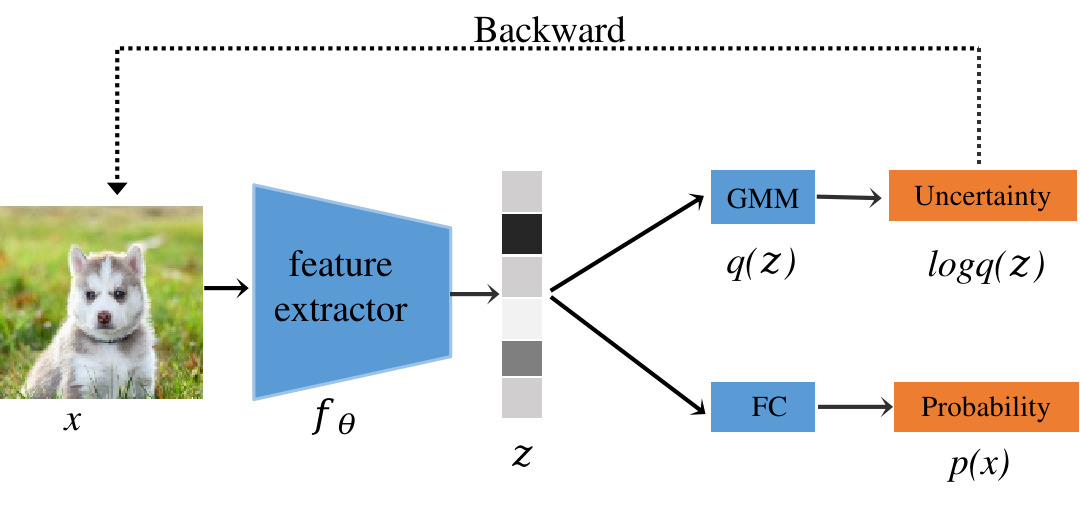
\includegraphics[width=1.\linewidth]{assets/structure1.png}
    \caption{基于高维特征概率密度建模的模型不确定性}
    \label{tag:模型结构图1}
\end{figure}

% \begin{figure}[h]
%     \centering
%     \begin{tikzpicture}[
%         node distance=1.5cm and 1.5cm,
%         every node/.style={minimum height=1.2cm, text width=2.0cm, align=center},
%         feature/.style={fill=blue!20},
%         GDA/.style={fill=orange!50,text width={1.0cm}},
%         fc/.style={fill=orange!50,text width={1.0cm}},
%         softmax/.style={fill=orange!50},
%         output/.style={fill=gray!30},
%         arrow/.style={-{Stealth[scale=1.2]}},
%         backward/.style={dashed, red, thick} % 红色虚线样式
%     ]
%     % Nodes
%     \node (image) {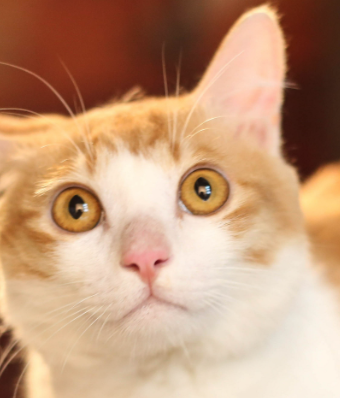
\includegraphics[width=1.5cm]{assets/cat.png}};
%     \node[below=0.2cm of image, align=center] (input_label) {输入$x$};
%     \node[feature, right=of image, trapezium, trapezium angle=60, fill=blue!20, minimum width=1.8cm, minimum height=1.5cm, shape border rotate=270] (feature_extractor) {feature extractor};
%     \node[below=0.2cm of feature_extractor, align=center] (input_label) {$f_\theta$};
    
%     % 条形图节点
%     \node[right=1cm of feature_extractor, inner sep=0] (bar_chart) {
%         \begin{tikzpicture}[scale=0.9]
%             % 绘制主条
%             \draw[thick] (0,0) rectangle (0.5,5); % 外框
%             % 分块填充
%             \fill[black!80] (0,4.5) rectangle (0.5,5);
%             \fill[gray!10] (0,4.0) rectangle (0.5,4.5);
%             \fill[gray!50] (0,3.5) rectangle (0.5,4);
%             \fill[black!70] (0,3) rectangle (0.5,3.5);
%             \fill[gray!70] (0,2.5) rectangle (0.5,3);
%             \fill[gray!20] (0,2) rectangle (0.5,2.5);
%             \fill[black!40] (0,1.5) rectangle (0.5,2);
%             \fill[gray!30] (0,1) rectangle (0.5,1.5);
%             \fill[black!80] (0,0.5) rectangle (0.5,1);
%             \fill[gray!60] (0,0) rectangle (0.5,0.5);
%         \end{tikzpicture}
%     };
%     \node[below=0.2cm of bar_chart, align=center] (input_label) {$z$};

%     % 其他节点
%     \node[GDA, above right=0.001cm and 0.5cm of bar_chart] (GDA) {GDA};
%     \node[below=0.1cm of GDA, align=center] (input_label) {$q(z)$};
%     \node[fc, below right=0.001cm and 0.5cm of bar_chart] (fc) {FC};
%     % \node[softmax, right=1.0cm of fc] (softmax) {Softmax};
%     \node[output, right=1.0cm of fc] (probs) {Probs};
%     \node[below=0.1cm of probs, align=center] (input_label) {$p(x)$};
%     \node[output, right=1.0cm of GDA] (logPx) {Uncertainty};
%     \node[below=0.1cm of logPx, align=center] (input_label) {$\log q(z)$};
    
%     % Paths
%     \draw[arrow] (image) -- (feature_extractor);
%     \draw[arrow] (feature_extractor) -- (bar_chart);
%     \draw[arrow] (bar_chart) -- (GDA);
%     \draw[arrow] (bar_chart) -- (fc);
%     \draw[arrow] (GDA) -- (logPx);
%     % \draw[arrow] (fc) -- (softmax);  
%     \draw[arrow] (fc) -- (probs);

%     % Backward path
%     \draw[backward] (logPx) -- ++(90:1.5cm) coordinate (midpoint); % 红色虚线
%     \draw[backward, ->] (midpoint) -- ++(180:10cm) node[pos=0.5, above] {Backward} -| (image); % 红色虚线

%     \end{tikzpicture}
%     \caption{基于高维特征概率密度建模的模型不确定性}
%     \label{tag:模型结构图}
% \end{figure}


\section{主要方法}
\subsection{不同样本梯度响应差异性研究}
Hendrycks等人\cite{hendrycks2017a}观察到训练好的网络倾向于给分布内样本一个相对更高的Softmax分数,进而提出一种无需重新训练网络的基线方法MSP,该方法使用Softmax分数表示不确定性,用于OOD检测任务。Shiyu Liang等人\cite{liang2017enhancing}在此基础上发现,在Softmax函数中使用温度缩放(temperature scaling),并且给输入加入微小的梯度相关的扰动,那么分布内样本和分布外样本的Softmax分数分布就会增大差异,进而显著提高OOD样本检测性能。Wang\cite{wang2023gradient}、Rui Huang\cite{huang2021importance}、Lee\cite{lee2020gradients}也在研究中指出梯度信息与模型的不确定性存在着相关性。本章在上述研究的启发下进一步研究分布内样本和分布外样本在梯度空间上分布的规律,实验结合理论推导,分析相关结论,最后通过添加与梯度相关的输入扰动,提高概率密度在建模神经网络模型不确定性上的效果。

本章有关神经网络的梯度空间的研究,是指神经网络反向传播时输出对输入图片求梯度。如图\ref{tag:模型结构图1},使用概率密度建模不确定性,训练好的神经网络一般有两个输出,一个是预测类别的概率$p(x)$,一个是计算模型不确定性的对数概率密度$\log q(z)$。本节分别研究了这两个输出关于输入的梯度,并通过梯度响应图的可视化分析$p(x)$和$\log q(z)$对梯度响应的区别。

首先,在梯度空间上对训练集样本和域外样本进行了统计分析,统计输出关于输入的梯度响应图。图\ref{fig:resp1}是在CIFAR10上训练的ResNet50可视化后的结果,选取SVHN和LSUN作为训练集以外的样本,计算出对数概率密度关于输入图片的梯度,得到的梯度张量在特征维度上求均值后的结果作为梯度响应图。可以看出对于训练集同分布的样本(上面一行),梯度响应普遍在比较小的范围,而对于训练集以外的样本(域外样本,下面一行,理论上来说这些样本的预测不确定性更高),梯度响应会更大,这个现象表明在关于输入的梯度空间上存在着能表征不确定性的信息。
\begin{figure}[h]
    \captionsetup{font=small, justification=centering}
    \centering
    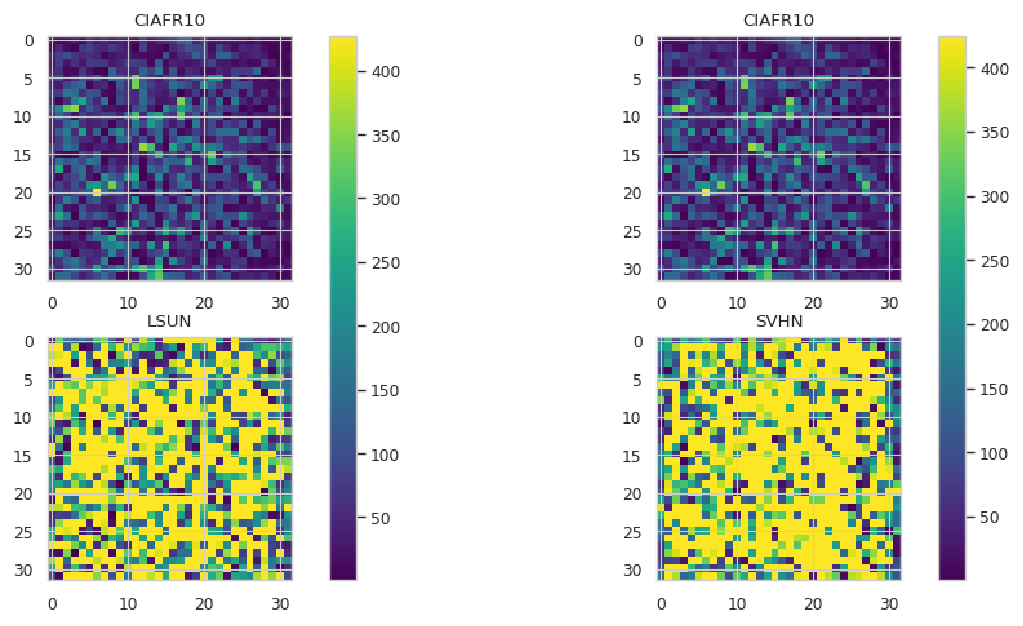
\includegraphics[width=0.75\linewidth]{assets/3-1.png}
    \caption{ResNet50 ,训练集 CIFAR10 vs OOD数据集LSUN、SVHN,可视化对数概率密度关于输入的梯度响应图
}
    \label{fig:resp1}
\end{figure}

图\ref{fig:resp2}是在CIFAR10上训练的ViT网络可视化梯度响应的结果,同样也是选取SVHN和LSUN作为训练集以外的样本,计算出概率密度关于输入的梯度作为梯度响应图。同样可以看出,对于基于Transformer\cite{vaswani2017attention}结构的神经网络,也有和卷积网络相同的结论,即对于训练集上的样本,关于输入的梯度响应在比较小的范围,而对于训练集以外的样本,关于输入的梯度响应会在一个更大的范围内。所以可以得出结论,对于基于Transformer结构的神经网络,关于输入的梯度空间上的信息也和模型不确定性具有相关性。
\begin{figure}[h]
    \captionsetup{font=small, justification=centering}
    \centering
    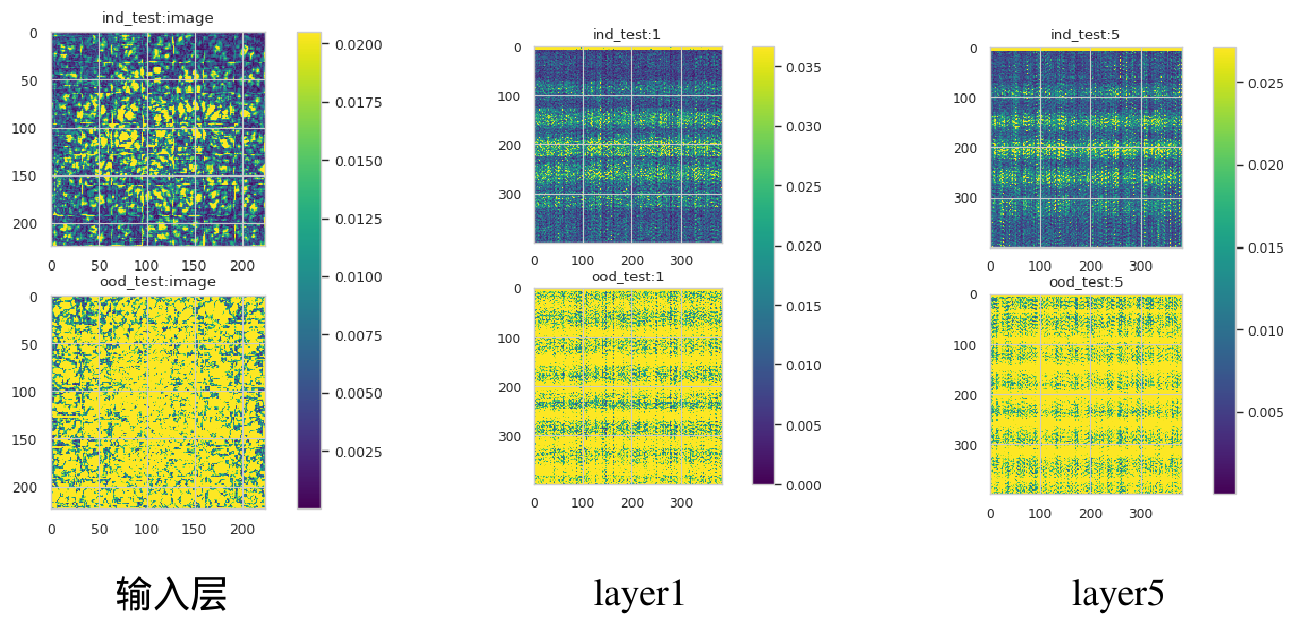
\includegraphics[width=0.75\linewidth]{assets/3-2.png}
    \caption{ViT,训练集 CIFAR10 vs OOD数据集LSUN、SVHN,可视化对数概率密度关于输入的梯度响应图
}
    \label{fig:resp2}
\end{figure}

以上研究了对不同网络结构使用概率密度求关于输入的图片梯度响应的结果,如上文所言,还可以计算经过Softmax输出的预测概率对输入图片求梯度,本节同样在实验中也可视化了Softmax计算出的预测概率对输入图片的梯度。图\ref{fig:resp3}是在CIFAR10上训练的ResNet50网络可视化梯度响应的结果,同样也是选取SVHN和LSUN作为训练集以外的样本,在这个实验中计算预测概率关于输入的梯度作为梯度响应图。同样可以看出,对于训练集上的样本,梯度响应落在比较小的范围内,而对于训练集以外的样本,梯度响应会在一个更大的范围内。对比图\ref{fig:resp1},同时可以发现,使用概率密度计算出来的梯度空间上的响应图,训练集和域外样本的分布差异更大,这表明使用对数概率密度计算出的梯度在表征不确定性上相比使用预测概率计算出来的梯度效果更好。
\begin{figure}[h]
    \captionsetup{font=small, justification=centering}
    \centering
    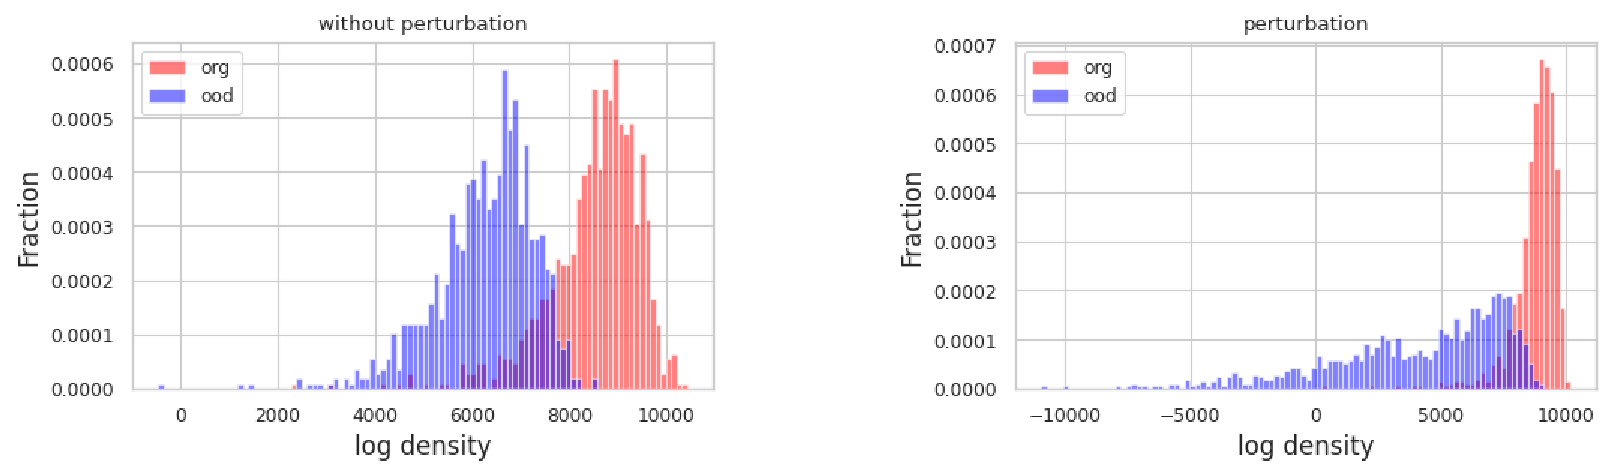
\includegraphics[width=0.75\linewidth]{assets/3-3.png}
    \caption{ResNet50,训练集 CIFAR10 vs OOD数据集LSUN、SVHN,可视化预测概率关于输入的梯度响应图
}
    \label{fig:resp3}
\end{figure}


上面通过实验定性地观察到了对于分布内样本和分布外样本,梯度空间上存在着明显的分布差异。为了定量地分析梯度空间上的信息在建模神经网络模型不确定性上效果,本节在实验中使用计算出来的梯度张量的范数作为模型不确定性的度量,并以在OOD检测任务上的表现作为评估。

实验中在CIFAR10数据集上分别训练VGG16、ResNet50和ViT模型,直接使用概率密度关于输入的梯度的范数作为模型不确定性的度量,选取SVHN、LSUN、CIFAR100、MNIST数据集作为分布外样本,在OOD检测任务上进行评估,选取DDU算法作为基线方法,对比了DDU算法和梯度范数(GradNorm)在OOD检测任务上的表现,通过AUROC和AUPRC两个指标评估它们在OOD检测任务上的效果,并以此间接地反映对模型不确定性的建模能力。实验结果如表\ref{tag:gradNorm}。
\begin{table}[h]
    \captionsetup{font=small, justification=centering}
    \centering
    \renewcommand{\arraystretch}{1.0} % Adjust line spacing
    \resizebox{\linewidth}{!}{
    \begin{tabular}{l l c c c}
    \toprule
    Method & OOD Dataset & VGG16+CIFAR10 & ResNet50+CIFAR10 & ViT+CIFAR10 \\
    &  & (Accuracy=0.9390) & (Accuracy=0.9558) & (Accuracy=0.9732) \\
    \midrule
    \multirow{4}{*}{DDU} 
    & SVHN & \textbf{0.9320} / \textbf{0.9480} & 0.9179 / 0.9415 &\textbf{ 0.9767} / \textbf{0.9835} \\
    & LSUN & \textbf{0.9160 }/ 0.9274 & \textbf{0.9239} /\textbf{ 0.9390} & \textbf{0.9858} /\textbf{ 0.9886} \\
    & CIFAR100 &\textbf{ 0.8932} / \textbf{0.9030} & \textbf{0.8888 }/\textbf{ 0.9018} & \textbf{0.9576} / \textbf{0.9534} \\
    & MNIST &\textbf{ 0.9195 }/ \textbf{0.9225 }& \textbf{0.9292 }/\textbf{ 0.9511 }& \textbf{0.9601 }/ \textbf{0.9684} \\
    \midrule
    \multirow{4}{*}{GradNorm} 
    & SVHN & 0.9308 / 0.9466 & \textbf{0.9282} / \textbf{0.9506} &  0.9325 / 0.9493 \\
    & LSUN & 0.9155 / \textbf{0.9326} & 0.9079/ 0.9300 & 0.8187 /  0.8755 \\
    & CIFAR100 & 0.8898 / 0.8987 & 0.8790 / 0.8955 & 0.9463/ 0.9495 \\
    & MNIST & 0.9010 / 0.9082 & 0.8958/ 0.9248 & 0.6787 / 0.7923 \\
    \bottomrule
    \end{tabular}
    }
    \caption{在CIFAR10上训练不同的模型(VGG16、ResNet50、ViT),选取SVHN、LSUN、CIFAR100、MNIST作为OOD样本,对比DDU算法和梯度范数(GradNorm)对模型不确定性的建模效果,报告指标是AUROC($\uparrow$) / AUPRC($\uparrow$)}
    \label{tag:gradNorm}
\end{table}


从实验结果来看,无论是对于卷积网络结构的VGG16、ResNet50模型,还是基于Transformer结构的ViT模型,都可以观察到,概率密度关于输入的梯度的范数可以作为OOD检测指标并具有良好的表现,这说明概率密度关于输入的梯度对模型的不确定性具有一定的建模能力,但是对比DDU方法对OOD检测任务上的表现可以看到,DDU方法在几乎所有数据集上均表现优异,AUROC/AUPRC值均高于梯度范数在OOD检测任务上的表现,这说明直接使用梯度范数作为不确定性的度量效果不如DDU算法。

针对上面观察到的分布内样本和分布外样本在梯度空间上的分布差异,下面尝试从理论上进行分析和解释。首先,关于对数概率密度关于输入的梯度有以下结论:

\textbf{性质1:}
假设$x$是输入图片,$f_\theta(x)$是神经网络特征提取部分, 高维特征\( z = f_\theta(x) \), 在高维特征上建立多元高斯分布\( q(z) = N(z|\mu_c, \Sigma_c) \),以及 模型不确定性为:\( U(x) = \log q(z) \)。那么 \( U(x) \) 对 \( x \) 的梯度 :
\[
\nabla_x U(x) = - \frac{\partial z}{\partial x}^T \Sigma_c^{-1} \left( z - \mu_c \right)
\]

\textbf{证明1:}根据 \( q(z) \) 的定义为正态分布的概率密度函数可知:
\[
q(z) = N(z|\mu_c, \Sigma_c) = \frac{1}{(2\pi)^{D/2}|\Sigma_c|^{1/2}} \exp\left(-\frac{1}{2}(z - \mu_c)^T \Sigma_c^{-1} (z - \mu_c) \right)
\]


\( U(x) = \log q(z) \) 的取对数展开后:
\[
U(x) = \log q(z) = -\frac{D}{2} \log(2\pi) - \frac{1}{2} \log |\Sigma_c| - \frac{1}{2}(z - \mu_c)^T \Sigma_c^{-1} (z - \mu_c)
\]


令 \( z = f_\theta(x) \),则 \( \nabla_x z = \frac{\partial z}{\partial x} = J \),其中 \( J \) 是 \( z \) 对 \( x \) 的雅可比矩阵。

\( U(x) \) 中与 \( x \) 相关的部分为:
\[
-\frac{1}{2}(z - \mu_c)^T \Sigma_c^{-1} (z - \mu_c)
\]

对 \( x \) 求梯度:
\[
\nabla_x U(x) = -\frac{1}{2} \nabla_x \left[ (z - \mu_c)^T \Sigma_c^{-1} (z - \mu_c) \right]
\]

对括号内的二次型展开:
\[
(z - \mu_c)^T \Sigma_c^{-1} (z - \mu_c) = \text{tr} \left[ \Sigma_c^{-1} (z - \mu_c) (z - \mu_c)^T \right]
\]

利用链式法则:
\[
\nabla_x \left[ (z - \mu_c)^T \Sigma_c^{-1} (z - \mu_c) \right] = 2 J^T \Sigma_c^{-1} (z - \mu_c)
\]

因此:
\[
\nabla_x U(x) = -J^T \Sigma_c^{-1} (z - \mu_c)
\]

最终结果可以写为:
\[
\nabla_x U(x) = - \frac{\partial z}{\partial x}^T \Sigma_c^{-1} \left( z - \mu_c \right)
\]

其中:\( z = f_\theta(x) \),\( J = \frac{\partial z}{\partial x} \) 是雅可比矩阵,\( \Sigma_c^{-1} \) 是协方差矩阵的逆,\( \mu_c \) 是均值向量。

分析上述推导结果,第一项主要是神经网络参数有关,由于对不同的输入统一使用训练好的确定网络,参数也是确定的,所以在分析分布内样本和分布外样本的梯度响应时,重要的因素是 \( (z - \mu_c) \) 和 \( \Sigma_c^{-1} \) 的相互作用。 对于分布内样本,其 \( z \) 接近于类别的均值 \( \mu_c \)。由于 \( z \) 离均值较近,\( (z - \mu_c) \) 的值较小,从而导致梯度较小,即梯度响应会相对较弱。这是因为分布内的样本已经在类别的集中区域,因此梯度计算时主要影响的是样本到均值的微小偏差。对于分布外样本,其 \( z \) 会远离类别的均值 \( \mu_c \),导致 \( (z - \mu_c) \) 的值较大。此时,梯度的响应较强,因为样本 \( z \) 相对于均值的距离较大。换句话说,分布外样本的梯度响应较高,因为它们距离类别中心较远,模型不确定性对于这些样本的变化响应更为显著。


\subsection{基于输入扰动的改进}
基于上一节关于不同分布的样本在梯度空间上的实验观察和理论分析,可以知道域内样本和域外样本在梯度空间上的分布存在着明显差异,在域内测试样本上概率密度对输入图片的梯度响应处在一个很低的范围内,而域外测试样本概率密度对输入图片的梯度响应处在一个很高的范围。基于梯度空间上域内样本和域外样本存在的分布差异,本节对基于高维特征概率密度估计的模型不确定性建模思路提出基于输入扰动的改进,基本思想是由于域内样本梯度响应比较小而域外样本梯度响应比较大,同时对输入图片加入与梯度相关的输入扰动,对域外样本的影响更大,偏离在训练集上所构建的经验分布,进而导致域内样本和域外样本在所构建分布上的分布差异将会变大。

基于高维特征概率密度估计的神经网络模型不确定性的建模,可以通过高斯判别分析模型建模高维特征空间的概率分布。高斯判别分析(Gaussian Discriminant Analysis,GDA)是一种经典的统计学方法,用于分类问题的建模。它假设数据的每个类别都服从高斯分布,并通过最大化似然函数来估计每个类别的高斯分布参数,从而进行分类。GDA假设每个类别的样本在特征空间中服从高斯分布。每个类别的特征向量被认为是从高斯分布中采样的,即每个类别的特征向量服从 \( N(\mu_k, \Sigma_k) \),其中 \( \mu_k \) 是第 \( k \) 类的均值向量,\( \Sigma_k \) 是第 \( k \) 类的协方差矩阵。对于每个类别 \( k \),其先验概率 \( P(C_k) \) 表示类别 \( k \) 出现的概率,通常通过训练数据中的类别频率来估计。



GDA通过最大化似然函数来拟合数据,即对每个类别估计一个高斯分布。其步骤可以总结为:

1. \textbf{估计均值和协方差}:给定类别标签 \( C_k \),对于每个类别,GDA计算其特征数据的均值向量和协方差矩阵:
   \[
   \mu_k = \frac{1}{N_k} \sum_{i=1}^{N_k} \mathbf{z}_i, \quad \Sigma_k = \frac{1}{N_k} \sum_{i=1}^{N_k} (\mathbf{z}_i - \mu_k)(\mathbf{z}_i - \mu_k)^T
   \]
   其中,\( N_k \) 是类别 \( k \) 的样本数量,\( \mathbf{x}_i \) 是第 \( i \) 个样本。

2. \textbf{类别的后验概率}:根据贝叶斯定理,计算样本属于每个类别的后验概率:
   \[
   P(C_k|\mathbf{z}) = \frac{P(\mathbf{z}|C_k) P(C_k)}{P(\mathbf{z})}
   \]
   其中,\( P(\mathbf{z}|C_k) \) 是给定类别 \( C_k \) 下数据点 \( \mathbf{z} \) 的条件概率密度,即高斯分布的概率密度函数:
   \[
   P(\mathbf{z}|C_k) = \frac{1}{(2\pi)^{d/2} |\Sigma_k|^{1/2}} \exp\left(-\frac{1}{2} (\mathbf{z} - \mu_k)^T \Sigma_k^{-1} (\mathbf{z} - \mu_k)\right)
   \]
   \( d \) 是特征的维度,\( |\Sigma_k| \) 是协方差矩阵的行列式,\( \Sigma_k^{-1} \) 是协方差矩阵的逆。

% 3. \textbf{分类决策}:在预测时,GDA根据后验概率来选择最可能的类别:
%    \[
%    \hat{y} = \arg\max_k P(C_k|\mathbf{z})
%    \]
%    由于 \( P(\mathbf{z}) \) 在所有类别中是相同的,因此可以省略不计,仅考虑 \( P(\mathbf{z}|C_k) P(C_k) \) 的最大值。



% \begin{equation}
% N(z|\mu_c,\Sigma_c)=\frac{1}{(2\pi)^{D/2}}\frac{1}{\left| \Sigma_c \right|^{1/2}}exp\left\{-\frac{1}{2}(z-\mu_c)^T\Sigma_c^{-1}(z-\mu_c)\right\}
% \end{equation}
% \begin{equation}
%     q(z)  = \sum_{c=1}^{K}w_cN(z|\mu_c,\Sigma_c)
% \end{equation}
% 利用测试样本在所建概率分布上的概率密度来评估模型的不确定性
在基于高维特征概率密度估计的模型不确定性建模中,本文使用最大类别后验概率计算模型不确定性,

\begin{equation}
    q(z)  = \max_c    P(C_k|\mathbf{z})  = \max_c \frac{P(\mathbf{z}|C_k) P(C_k)}{P(\mathbf{z})}
\end{equation}
对于类别均匀的训练样本,等价于使用下面的表达式计算模型不确定性:
\begin{equation}
    q(z)  = \max_c P(\mathbf{z}|C_k)  =  \max_c N(z|\mu_c,\Sigma_c)
\end{equation}

对基于高维特征概率密度估计的模型不确定性的研究,本节提出基于输入扰动的改进策略。具体而言,在\textbf{训练阶段},需要首先训练一个高准确率的神经网络,使用训练好的骨干网络对训练集上的图片提取高维特征以生成训练样本的特征表示,然后为每个类别计算其高维特征的均值$\mu_c$、协方差矩阵$\Sigma_c$以及类别先验概率$q(y|c)$,从而建立一个描述特征空间分布的高斯判别分析模型$q(z)$。

在\textbf{不确定性计算阶段},通过特征提取网络计算测试样本$x$的高维特征表示$z$,并利用高斯判别分析模型估计该高维特征$z$的概率密度$\log q(z)$。 随后,对输入样本施加梯度有关的输入扰动(
添加输入扰动的方式见公式\ref{perturb})

\begin{equation}
    \tilde{x}=x+\epsilon* \cdot (-\nabla_x U(x))
    \label{perturb}
\end{equation}
其中:
\begin{equation}
    U(x)=\log q(f_{\theta}(x))
\end{equation}
超参数$\epsilon$控制添加的输入扰动的强度,可以通过网格搜索(Grid Search)优化得到最优的值。


得到扰动后的输入$\tilde{x}$,使其沿着概率密度减小的方向变化,并将扰动后的输入$\title{x}$重新送入神经网络,再次计算扰动后样本的概率密度$q(\tilde{z})$,扰动后的概率密度最终作为模型在该输入样本上的模型不确定性度量:$Uncertainty(x) = logq(\tilde{z})$。完整的基于输入扰动的改进算法原理见算法\ref{alg:1}。

\begin{algorithm}[h]
	\caption{基于输入扰动的概率密度建模的模型不确定性算法}
	\label{alg:1}
	
	\begin{algorithmic}[1]
		\Require 训练集: $(X,Y)$ 
		\Require 谱归一化的高维特征提取网络: $f_{\theta}:x \rightarrow \mathbf{R}^d $ 
		\Require GDA模型: $q(z) = \max_{c}q(z|y=c)$
		
		\\
		\Procedure {1.训练阶段和GDA建模}{}
		\State 在训练数据集数据集上训练网络$f_{\theta}$
		\For {属于类别c的样本}
		\State $\mu_{c}=\frac{1}{|x_c|}f_{\theta}(x_c)$
		\State $\Sigma_c = \frac{1}{|x_c|-1}(f_{\theta}(x_c)-\mu_c)(f_{\theta}(x_c)-\mu_c)^T$
		\State q(y=c)=$\frac{|X_C|}{|X|}$
		\EndFor
		\EndProcedure

		
		\\
		\Procedure {2.模型不确定性计算}{}
		\State $z=f_{\theta}(x)$
		\State  $q(z) = \max_{c}q(z|y=c)$,其中$q(z)\sim N(\mu_c,\Sigma_c)$
		\State 输入扰动:$\tilde{x}=x+\epsilon* \cdot (-\nabla_x \log q(z)))$,其中$\epsilon$是扰动系数
		\State $\tilde{z}=f_{\theta}(\tilde{x})$
		\State 计算模型不确定性 $Uncertainty(x) = \log \max_{c}q(\tilde{z}|y=c)$,其中$q(\tilde{z})\sim N(\mu_c,\Sigma_c)$
		\EndProcedure 
	\end{algorithmic}
\end{algorithm}


下面通过可视化加入输入扰动前后对数概率密度的分布直方图,分析加入输入扰动对模型不确定性的影响。选取一批训练集同分布的图片和一批分布外的图片作为测试输入,对输入图像按照上面提出的扰动方式添加梯度相关的扰动,并重新计算了对数概率密度作为模型不确定性的度量,在直方图中可视化不确定性的分布,对比加入输入扰动前后模型不确定性的分布。实验结果如图\ref{tag:uncertainty 1}所示。首先在CIFAR10数据集上训练了ResNet50模型,并用GDA模型在训练集提取的高维特征上建立了经验分布。选取CIFAR10数据集的测试集作为分布内样本(inD),SVHN、CIFAR100、MNIST、LSUN数据集的测试集作为分布外样本(OOD)。在扰动前,将图片送入ResNet50中计算高维特征,并计算在GDA中的对数概率密度作为模型不确定性。随后,对输入图片加入了与梯度相关的扰动,并同样地送入ResNet50网络模型和GDA分布中计算对数概率密度作为模型不确定性。左边是没有加入输入扰动时对于inD样本和OOD样本模型不确定性的分布,右边是加入输入扰动后模型不确定性的分布。红色分布是inD样本的模型不确定性分布曲线,蓝色分布是OOD样本的模型不确定性分布曲线。从图中可以看出,inD样本的概率密度处在一个较大的范围内分布,而OOD样本的概率密度在一个较小的数值范围内分布。加入输入扰动后,inD样本和OOD样本的模型不确定性同时减少,且两个分布的重合区域减小了,也就是说OOD样本和inD样本的模型不确定性分布差异在变大。

基于上述可视化结果,可以知道,通过加入与梯度相关的输入扰动,能够有效地增加OOD样本和inD样本在模型不确定性分布上的差异,从而可以更好地建模模型不确定性,提高模型对OOD样本的识别能力。



\begin{figure}[htbp]
    \vspace{-1pt} % 增加负值来减少上方的空白
    \centering
    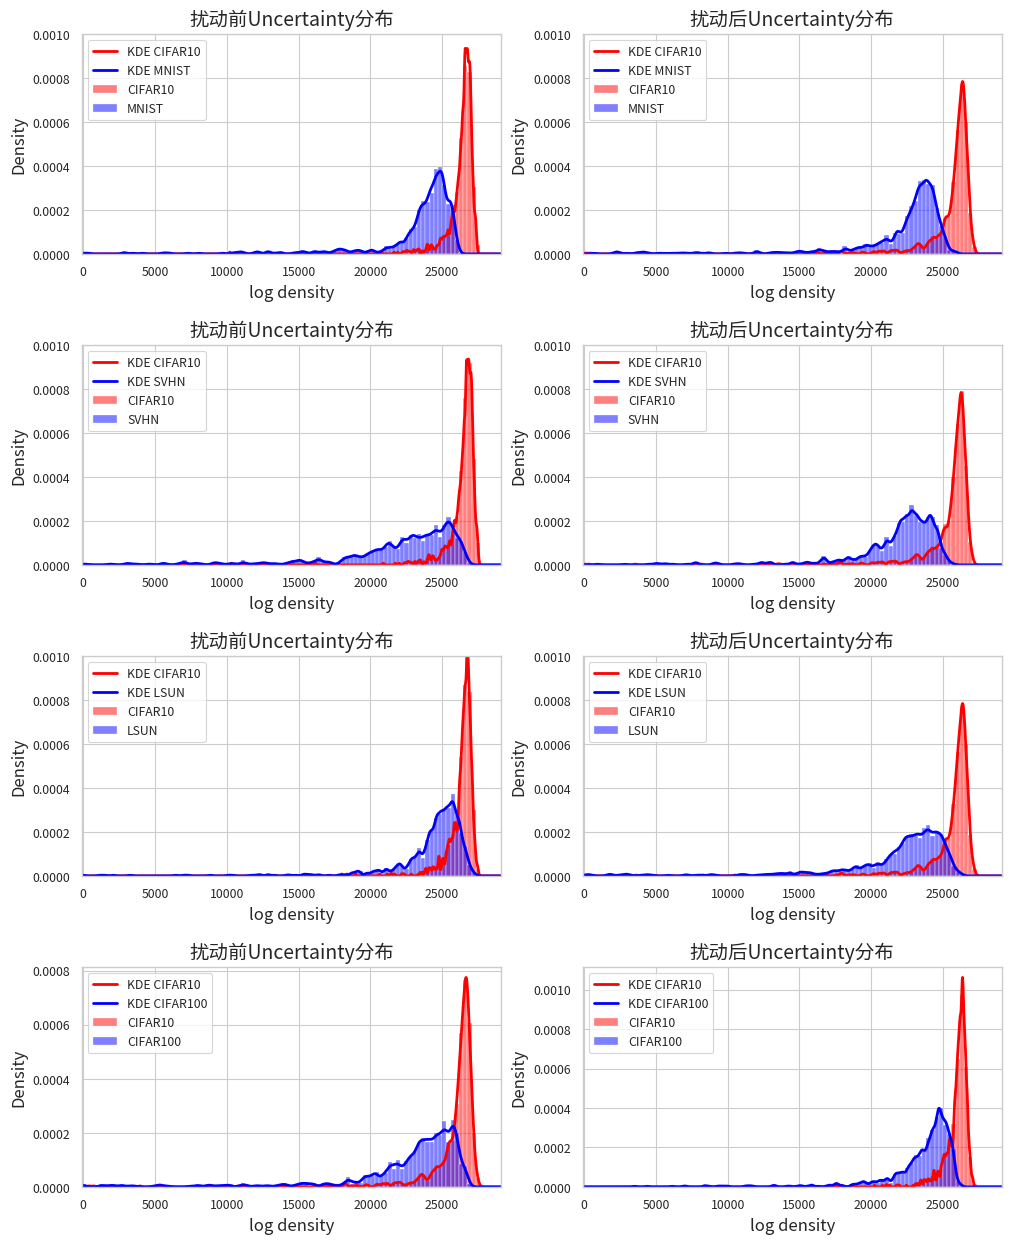
\includegraphics[width=\linewidth]{assets/combined_vertical_image.png}
    \vspace{-1pt} % 可以增加负值来减少下方的空白
    \caption{ResNet50模型 ,训练集 vs OOD数据集,模型不确定性的分布直方图}
    \label{tag:uncertainty 1}
\end{figure}
% \begin{figure}[H]
%     \vspace{-1pt} % 增加负值来减少上方的空白
%     \centering
%     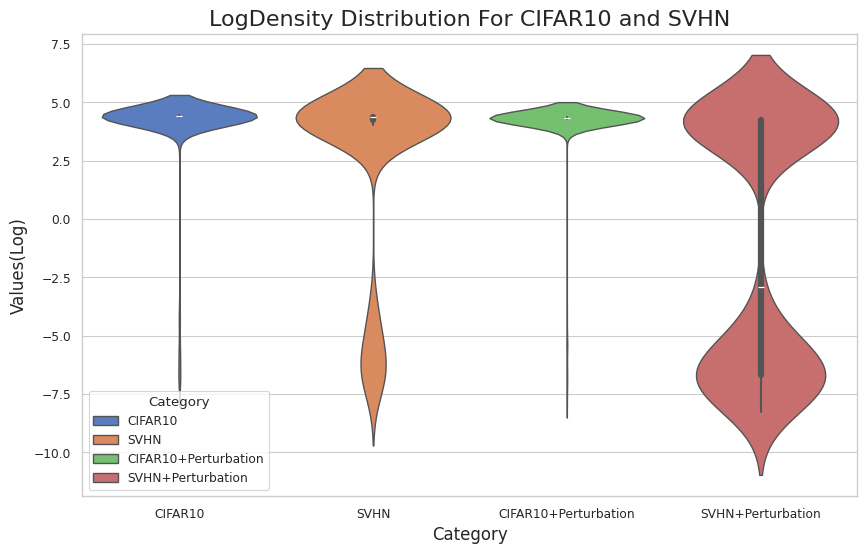
\includegraphics[width=\linewidth]{assets/SVHN_logdensity_violin_purturbation.png}
%     \caption{ResNet50 ,训练集 CIFAR10 vs OOD数据集SVHN,模型不确定性的分布小提琴图}
%     \label{tag:uncertainty 3}
% \end{figure}


% \ref{tag:uncertainty 3}这张图展示了CIFAR10和SVHN两种数据集的对数密度分布(LogDensity),以及添加扰动后的分布变化。原始数据中,CIFAR10的密度值集中在较高区域(0到5),分布紧凑,表明特征分布较为集中;而SVHN的密度范围更广(-7.5到5),分布较为分散,说明其特征噪声更大且类间区分性较低。添加扰动后,CIFAR10的分布范围有所扩展(-10到7.5),但中心变化不大,影响较小;相比之下,SVHN的分布变化更显著,扰动导致其密度分布更对称且范围更大,表明SVHN对扰动更为敏感。这说明CIFAR10特征分布较紧凑,更易分类,而SVHN分布较分散,模型可能需要更强的鲁棒性来应对扰动对特征区分性的影响。


当加入微小输入扰动时,关于对数概率密度的变化,有以下结论:

\textbf{性质2:}
假设$x$是输入图片,$f_\theta(x)$是神经网络特征提取部分, 高维特征\( z = f_\theta(x) \), 高维特征符合多元高斯分布\( q(z) =  N(z|\mu_c, \Sigma_c) \),以及 \( U(x) = \log q(z) \)。 \( U(x) \) 对 \( x \) 的梯度 \( \nabla_x U(x) \):\[
\nabla_x U(x) = - \frac{\partial z}{\partial x}^T \Sigma_c^{-1} \left( z - \mu_c \right)
\],对于输入 \( x \) 添加微小的梯度扰动, $\tilde{x}=x+\epsilon* (-\nabla_x U(x))$
,那么加上输入扰动后$\tilde{x}$概率密度下降,且$z$距离均值越远,下降程度越大。

\textbf{证明2:}

多元正态分布的概率密度函数为:
\[
N(z) = \frac{1}{\sqrt{(2\pi)^k |\Sigma|}} \exp\left(-\frac{1}{2}(z - \mu_c)^T \Sigma^{-1} (z - \mu_c)\right),
\]
取对数后可得:
\[
U(x) = \log N(z) = -\frac{k}{2} \log(2\pi) - \frac{1}{2} \log |\Sigma| - \frac{1}{2} (z - \mu_c)^T \Sigma^{-1} (z - \mu_c),
\]
其中 \( z = f(x) \)。

将 \( U(x+\delta) \) 在 \( x \) 附近进行一阶泰勒展开:
\[
U(x+\delta) \approx U(x) + \nabla U(x)^T \delta.
\]
因此:
\[
U(x+\delta) - U(x) \approx \nabla U(x)^T \delta.
\]

将 \( \delta = \epsilon* (-\nabla_x U(x)) \) 代入,得到:
\[
U(x-\epsilon \nabla U(x)) - U(x) \approx - \epsilon \nabla U(x)^T \nabla U(x).
\]

由于 \( \nabla U(x)^T \nabla U(x) \) 是梯度的二范数平方,故其始终非负:
\[
\|\nabla U(x)\|^2 = \nabla U(x)^T \nabla U(x) \geq 0.
\]
因此:
\[
U(x-\epsilon \nabla U(x)) - U(x) \leq 0.
\]

所以,添加相关扰动后,概率密度会下降。

根据\textbf{性质3.1},有:
\[
\nabla_x U(x) = - \frac{\partial z}{\partial x}^T \Sigma_c^{-1} \left( z - \mu_c \right).
\]

将其带入 \( -\nabla U(x)^T \nabla U(x) \),展开后可得:
\[
-\nabla U(x)^T \nabla U(x) = -\left[ -\frac{\partial z}{\partial x}^T \Sigma_c^{-1} \left( z - \mu_c \right) \right]^T \left[ -\frac{\partial z}{\partial x}^T \Sigma_c^{-1} \left( z - \mu_c \right) \right].
\]

化简后:
\[
U(x-\epsilon \nabla U(x)) - U(x) \approx
-\epsilon\nabla U(x)^T \nabla U(x) = -\epsilon\left( z - \mu_c \right)^T \Sigma_c^{-1} \frac{\partial z}{\partial x} \frac{\partial z}{\partial x}^T \Sigma_c^{-1} \left( z - \mu_c \right),
\]
其中中间的部分是正定的,所以$z$距离均值越远,降低程度越大。

结合上面的结论,下面从理论上分析加入与梯度相关的扰动是如何影响模型不确定性。已知模型不确定性对输入图像的梯度:
\[
\nabla_x U(x) = - \frac{\partial z}{\partial x}^T \Sigma_c^{-1} (z - \mu_c)
\]
这一梯度反映了模型不确定性 \( U(x) \) 如何随着输入 \( x \) 的变化而变化。在扰动过程中,向输入图像施加一个与梯度方向相关的扰动量 \( \epsilon \nabla_x U(x) \),因此新的图像变为  $\tilde{x}=x+\epsilon* (-\nabla_x U(x))$,即添加梯度反方向的输入扰动。通过这一扰动,神经网络提取的输入图像的特征 \( z \) 会发生变化。由于梯度方向是概率密度下降最快的方向,扰动后的图像 \( \tilde{x}\) 的特征 \( \tilde{z} \) 会更远离原始均值 \( \mu_c \)。这种调整意味着,扰动后的图像 \( \tilde{x}\) 将导致概率密度 \( U(x) \) 的值下降。这是因为当特征 \( \tilde{z} \) 远离均值 \( \mu_c \) 时,\( (\tilde{z} - \mu_c)^T \Sigma_c^{-1} (\tilde{z} - \mu_c) \) 的值增大,从而使得 \( U(\tilde{x}) \) 变得更低,表示模型对输入图像的不确定性增大。

具体到实验中的inD样本和OOD样本,扰动作用会影响它们的概率密度。对于inD样本,其特征 \( z \) 初始时与均值 \( \mu_c \) 较为接近,因此概率密度较大,模型的置信度较高。当施加扰动后,尽管扰动使得这些inD样本的特征 \( \tilde{z} \) 更远离均值,但由于它们本身已经较接近均值,扰动后的变化不会非常剧烈,导致其概率密度的下降幅度相对较小。

与此不同,OOD样本的特征 \( z \) 在原始状态下已经远离均值 \( \mu_c \),因此其初始概率密度较低,表现出较高的不确定性。当对这些样本施加扰动时,它们的特征 \( \tilde{z} \) 会进一步偏离均值,导致其概率密度迅速下降。由于这些样本初始就处于分布的边缘或尾部,扰动引起的概率密度变化更加显著,因此它们的模型不确定性增加幅度远大于inD样本。

通过这样的扰动作用,可以观察到inD样本和OOD样本的不确定性分布在扰动前后的变化。原本重叠较多的分布,经过扰动后,逐渐拉开了差距。尤其是扰动后,OOD样本的概率密度下降幅度更大,从而使得inD样本和OOD样本的模型不确定性分布差异显著增大。这表明,扰动不仅使得模型对OOD样本的敏感性更高,还提高了模型区分inD样本和OOD样本的能力。

综上所述,梯度扰动的加入使得输入图像的特征 \( z \) 更加偏离均值 \( \mu_c \),从而导致概率密度 \( U(x) \) 下降。对于OOD样本,由于其特征原本就远离均值,扰动的影响更为显著,导致其不确定性增大幅度大于inD样本,从而加大了两者之间的不确定性分布差异。



\section{实验结果与分析}
为了评估本文所提出的基于输入扰动的改进对模型不确定性建模的提升,本节分别在OOD检测任务上,对抗样本检测任务上,误分类样本识别,主动学习等任务上进行了评估。本节的实验内容主要是在CIFAR-10\cite{Krizhevsky2009},CIFAR-100\cite{Krizhevsky2009},SVHN\cite{Netzer2011},MNIST\cite{LeCun1998},LSUN\cite{Yu2015}等数据集和VGG\cite{simonyan2014very},ResNet\cite{he2016deep},ViT\cite{dosovitskiy2020image}等模型进行的,有关实验数据集和模型介绍如下:

\subsubsection{实验数据集介绍}


CIFAR-10(Canadian Institute for Advanced Research 10)是一个广泛用于机器学习和计算机视觉领域的小型图像分类数据集,主要设计用于图像分类任务和模型性能的评估。 CIFAR-10 包含 10 个类别的彩色图像,CIFAR10数据集包含训练集50000 张图片,每类 5000 张,测试集10000 张图片,每类 1000。每张图片的大小为 32 × 32 ,彩色图像。每张图片都有一个对应的标签,用于标注其所属的类别,标签值从 0 到 9,分别对应 10 个类别。

CIFAR-100 数据集是 CIFAR-10 的扩展版,也是一个广泛用于机器学习和计算机视觉任务的小型图像数据集。它具有更复杂的分类任务,适合评估和研究模型在多类别任务中的表现。 CIFAR-100 包含 100 个类别的彩色图像,每个类别的图片属于自然界和日常生活中的常见对象,例如植物、动物、交通工具等。CIFAR-100包含训练集50000 张图片,每类 500 张,测试集10000 张图片,每类 100 张。每张图片的大小为 32 × 32 ,彩色图片。CIFAR-100 提供两种标签:粗粒度标签有20 个粗类别(如哺乳动物、鱼类、家具等),每个粗类别下包含若干个细粒度类别。细粒度标签共100 个细类别,标签值从 0 到 99。

SVHN(Street View House Numbers)数据集是一个常用于机器学习和计算机视觉的公开数据集,主要设计用于识别自然场景中的数字。SVHN数据集由从谷歌街景图片中提取的数字组成,图片内容通常包含街道门牌号码中的数字。目标是识别每张图片中的数字类别(0-9)。SVHN数据集包含训练集73257 张图片,测试集26032 张图片,额外数据集531131 张图片,用于扩展训练数据,图片分辨率为32 × 32 ,都是彩色图片(RGB),标签范围0 到 9。

MNIST(Modified National Institute of Standards and Technology)数据集是机器学习和计算机视觉领域最著名的基准数据集之一,用于手写数字识别任务。 MNIST 数据集包含灰度的手写数字图片,数字范围为 0 至 9(共 10 个类别),训练集有60000 张图片,测试集有10000 张图片,每张图片的分辨率为 28 × 28 ,每张图片都有一个对应的标签,表示其数字类别,标签值为 0 到 9 的整数。


LSUN (Large-scale Scene Understanding) 是一个计算机视觉中的大规模的场景理解任务图像数据集,由中国香港中文大学的视觉计算组(CUImage)创建, 包含了数百万张图像,涵盖了10个不同的类别(如房间、建筑物、场景等),每个类别通常包含大量的标注图像,图像内容大多是场景中的自然环境或人工结构,适合用于训练场景分类、检测等任务。LSUN 分类数据集包含 10 个场景类别,例如餐厅、卧室、鸡、户外教堂等。对于训练数据,每个类别包含大约 120000 到 3000000张图片,验证数据集包括 300 张图像,测试数据集每个类别有 1000 张图像。


\subsubsection{实验模型介绍}
VGG 是由牛津大学 Visual Geometry Group 提出的经典卷积神经网络模型,因其结构简单而广受欢迎。VGG 的核心特点是使用多个 3×3 的小卷积核堆叠代替大卷积核,增加了网络的非线性表达能力,同时保持较少的参数量。VGG16 是其代表性版本,由 16 层有权重的层组成,包括 13 层卷积层和 3 层全连接层。尽管参数量较大(约 138M),VGG 模型凭借高效的特征提取能力,在图像分类和特征迁移任务中表现优异。

ResNet(Residual Network)由微软亚洲研究院提出,通过引入残差结构解决了深度网络中的梯度消失问题,使得网络可以加深到上百层甚至更深。其核心模块是残差块(Residual Block),通过跳跃连接(Skip Connection)将输入直接添加到输出,从而实现“学习残差”的目标。

ViT 是 Google 提出的首个将 Transformer 架构引入计算机视觉的模型,通过处理图像块实现全局特征建模。它将图像划分为固定大小的图块,展平后作为序列输入 Transformer 编码器,同时通过位置编码加入空间信息。ViT 擅长在大型数据集上捕获全局依赖关系,与传统卷积网络相比,更加灵活且具有更少的归纳偏置。尽管其对数据量和计算资源的要求较高,但 ViT 在图像分类等任务上展现了超越传统 CNN 的潜力。

本章主要训练了VGG16,ResNet50,ViT三种不同的神经网络模型,有关批次,批大小,优化器,初始学习率等超参数设置见下表格\ref{tab:模型训练}。
\begin{table}[htbp]
	\captionsetup{font=small, justification=centering}
	\centering
	\resizebox{\linewidth}{!}{
	\begin{tabular}{c c c c c c c c}
	\hline
	模型结构 & 训练数据集 & 批次 & 批大小 &优化器 & 初始学习率 & 动量 &权重衰减 \\
	\hline
	VGG16 & CIFAR10 & 300 & 512 & SGD & 0.1 & 0.9 & 0.0005 \\
        ResNet50 & CIFAR10 & 300 & 512 & SGD & 0.1 & 0.9 & 0.0005 \\
        ViT & CIFAR10 & 300 & 512 & SGD & 0.01 & 0.9 & 0.0005 \\
	\hline
	\end{tabular}
	}
	\caption{
	模型训练超参数设置
	}
        \label{tab:模型训练}
\end{table}



\subsection{OOD检测任务上评估}
OOD检测任务是指在机器学习和深度学习领域中,模型需要识别输入数据是否属于其训练数据分布范围的任务。OOD样本通常是训练过程中未见过的、不属于目标分布的输入数据,可能来源于其他类别、分布或完全不同的数据集。对于训练集上的分布内样本(In-Distribution, InD)通常具有较低的不确定性,而对于分布外样本(OOD)由于未被训练数据覆盖,模型对其预测的可信度应该较低,应表现为高不确定性。因此,模型不确定值作为OOD检测的指标是否能否有效地区分ID和OOD样本,可以间接地反映所计算出来的不确定性的值对模型不确定性的建模效果,利用模型不确定性检测OOD样本的规则如\ref{eq:uncertainty_rule}所示。

本章实验首先是在OOD检测任务上评估基于输入扰动的改进对模型不确定性建模的效果,在CIFAR10数据集的训练集上训练分类模型,选取CIFAR10测试集作为分布内样本,然后选取SVHN,LSUN,MNIST,CIFAR100等数据集作为分布外样本,使用计算出来的概率密度作为模型不确定性并进行OOD检测,对比扰动前后的不确定性建模的效果。实验结果如表\ref{tag:ood_results_cifar}。

\begin{equation}
x {\rightarrow}
\begin{cases} 
\text{in-domain (inD)} & \text{if } Uncertainty(x) < threshod, \\
\text{out-of-domain (OOD)} & \text{if } Uncertainty(x) > threshold.
\end{cases}
\label{eq:uncertainty_rule}
\end{equation}



\begin{table}[h]
    \captionsetup{font=small, justification=centering}
    \centering
    \renewcommand{\arraystretch}{1.0} % Adjust line spacing
    \resizebox{\linewidth}{!}{
    \begin{tabular}{l l c c c}
    \toprule
    Method & OOD Dataset & VGG16+CIFAR10 & ResNet50+CIFAR10 & ViT+CIFAR10 \\
    &  & (Accuracy=0.9390) & (Accuracy=0.9558) & (Accuracy=0.9732) \\
    \midrule
    \multirow{4}{*}{DDU} 
    & SVHN & \textbf{0.9320} / \textbf{0.9480} & 0.9179 / 0.9415 & 0.9767 / 0.9835 \\
    & LSUN & 0.9160 / \textbf{0.9274} & 0.9239 /0.9390 & 0.9858/0.9886\\
    & CIFAR100 & 0.8932 / 0.9030& 0.8888 / 0.9018 & 0.9476 /\textbf{0.9534} \\
    & MNIST & 0.9195 / 0.9225 & 0.9292 /0.9511& 0.9601 / 0.9684\\
    \midrule
    \multirow{4}{*}{输入扰动的改进方法} 
    & SVHN & 0.9283 / 0.9455 & \textbf{0.9690} / \textbf{0.9731} & \textbf{ 0.9828} / \textbf{0.9867} \\
    & LSUN & \textbf{0.9172} / 0.9266 & \textbf{0.9323}/ \textbf{0.9411} &\textbf{ 0.9929} / \textbf{ 0.9938} \\
    & CIFAR100 & \textbf{0.8938} /\textbf{ 0.9047} &\textbf{ 0.8898} / \textbf{0.9026} & \textbf{0.9491}/ 0.9529 \\
    & MNIST &\textbf{ 0.9482 }/ \textbf{0.9407} & \textbf{0.9757}/ \textbf{0.9813} & \textbf{0.9903 }/ \textbf{0.9919 }\\
    \bottomrule
    \end{tabular}
    }
    \caption{在CIFAR10上训练不同的模型(VGG16,ResNet50,ViT),选取SVHN、LSUN、CIFAR100、MNIST作为OOD样本,对比DDU算法和本章提出的输入扰动的改进对模型不确定性的建模效果,报告指标是AUROC($\uparrow$) / AUPRC($\uparrow$)}
    \label{tag:ood_results_cifar}
\end{table}


从实验结果中可以看出,相比与DDU算法,基于输入扰动的改进在大多数情况下显著提升了OOD 检测性能,在 AUROC 和 AUPRC 两项指标上的表现均优于基础 DDU 方法。实验在不同的模型(VGG16、ResNet50 和 ViT)和 OOD 数据集(如 SVHN、LSUN、CIFAR100 和 MNIST)上,输入扰动均提升了OOD检测的效果。此外,还可以观察到,模型架构对OOD检测结果也有显著影响,ViT 模型在整体表现上优于 VGG16 和 ResNet50,这可能归因于其更复杂的网络具备更强的表征学习能力。综合来看,输入扰动的策略作为对 DDU 方法的改进,不仅提升了模型的不确定性建模能力,还在多种场景下展示了其对鲁棒性的显著作用,具有重要的应用潜力。

在实验中,还选取MNIST数据集作为训练集,在VGG16/ResNet等模型上训练,并选取CIFAR10/LSUN/CIFAR100/SVHN作为OOD数据集进行OOD检测,从表\ref{tab:ood_results_mnist}中同样可以看出输入扰动的改进计算出来的不确定性在OOD检测任务上带来的提升,验证了基于输入扰动的改进策略对模型不确定性建模能力的提升。
\begin{table}[h]
    \captionsetup{font=small, justification=centering}
    \centering
    \renewcommand{\arraystretch}{1.0} % Adjust line spacing
    \resizebox{\linewidth}{!}{
    \begin{tabular}{l l c c}
    \toprule
    Method & OOD Dataset & VGG16+MNIST (Accuracy=0.9882) & ResNet50+MNIST (Accuracy=0.9870) \\
    \midrule
    \multirow{4}{*}{DDU} 
    & CIFAR10 & 0.9949 / 0.9964 & 0.9949 / 0.9964 \\
    & LSUN & 0.9946 / 0.9962 & 0.9946 / 0.9962 \\
    & CIFAR100 & 0.9945 / 0.9961 & 0.9945 / 0.9961 \\
    & SVHN & 0.9941 / 0.9960 & 0.9941 / 0.9960 \\
    \midrule
    \multirow{4}{*}{输入扰动的改进方法} 
    & CIFAR10 & \textbf{0.9965} / \textbf{0.9974} & \textbf{0.9965} / \textbf{0.9974} \\
    & SVHN & \textbf{0.9963} / \textbf{0.9972} & \textbf{0.9963} / \textbf{0.9972} \\
    & CIFAR10 & \textbf{0.9961} / \textbf{0.9970} & \textbf{0.9961} / \textbf{0.9970} \\
    & SVHN & \textbf{0.9964} / \textbf{0.9973} & \textbf{0.9964} / \textbf{0.9973} \\
    \bottomrule
    \end{tabular}
    }
    \caption{在MNIST上训练不同的模型(VGG16,ResNet50),选取SVHN、LSUN、CIFAR100、CIFAR10作为OOD样本,对比DDU算法和基于输入扰动的改进对模型不确定性的建模效果,报告指标是AUROC($\uparrow$) / AUPRC($\uparrow$)}
    \label{tab:ood_results_mnist}
\end{table}



\subsubsection{与各种主流不确定性建模方法的对比}
在本节设计实验,对比所提出的基于输入扰动的改进策略和各种主流的不确定性建模方法。在实验中,使用ResNet50模型在CIFAR10数据集上进行训练,选取不同数据集(CIFAR100、LSUN、MNIST和SVHN)作为OOD样本,并通过对比几种常用的不确定性建模的方法在OOD检测任务上的表现,来观察基于输入扰动的改进所带来的提升。实验中选择了四种不确定性建模方法:MSP、集成方法(Ensemble)、DDU和 本文提出的基于输入扰动的改进方法,并以AUROC和AUPRC作为评价OOD检测的指标,越高说明对不确定性建模效果越好,实验中MSP方法使用最大Softmax概率作为不确定性的度量,模型集成类方法在不同的数据集增强策略和参数初始化条件下训练了5个模型,模型集成方法使用多次预测的概率的熵作为不确定性的度量,DDU算法和基于输入扰动的改进方法都是在训练集上建模GDA分布并使用测试样本的概率密度作为不确定性的度量。所有的实验结果见表\ref{tab:不同方法的对比}。


从实验结果可以看出,DDU算法作为单一确定性神经网络建模不确定性的算法,虽然具有存储空间小和计算高效等优点,但是对不确定性建模的效果相比模型集成类的方法还有差距,整体上来看模型集成类的算法在OOD检测任务上表现是优于DDU算法的。同时可以观察到,加入输入扰动后,在OOD检测任务上在多个数据集上取得了最佳的AUROC/AUPRC值,甚至在MNIST和SVHN数据集上超过了过去最优的建模不确定性的算法模型集成类的方法。综合实验结果,可以得出结论:输入扰动的改进方法在OOD检测任务中显著优于传统的MSP和DDU算法,提升了对不确定性的建模能力。


\begin{table}[htbp]
	\captionsetup{font=small, justification=centering}
	\centering
	\resizebox{\linewidth}{!}{
	\begin{tabular}{c c c c c}
	\hline
	inD/OOD Dataset & 方法 & 不确定性计算方式 & AUROC & AUPRC \\
	\hline
	\multirow{4}{*}{CIFAR10/CIFAR100} & MSP & 最大预测概率 & 0.8925 & 0.8995 \\
	 & Ensemble & 熵 & \textbf{0.9184} & \textbf{0.9167} \\
	 & DDU & 概率密度 & 0.8888 & 0.9018 \\
	 & \textbf{输入扰动的改进} & 概率密度 & 0.8898 & 0.9026 \\
	\hline
	\multirow{4}{*}{CIFAR10/LSUN} & MSP & 最大预测概率 & 0.9120 & 0.9238 \\
	 & Ensemble & 熵 & \textbf{0.9401} & 0.9265 \\
	 & DDU & 概率密度 & 0.9239 & 0.9390 \\
	 & \textbf{输入扰动的改进} & 概率密度 & 0.9323 & \textbf{0.9411} \\
	\hline
	\multirow{4}{*}{CIFAR10/MNIST} & MSP & 最大预测概率 & 0.9471 & 0.9573 \\
	 & Ensemble & 熵 & 0.9735 & 0.9706 \\
	 & DDU & 概率密度 & 0.9292 & 0.9511 \\
	 & \textbf{输入扰动的改进} & 概率密度 & \textbf{0.9757} & \textbf{0.9813} \\
	\hline
	\multirow{4}{*}{CIFAR10/SVHN} & MSP & 最大预测概率 & 0.9392 & 0.9405 \\
	 & Ensemble & 熵 & 0.9667 & 0.9599 \\
	 & DDU & 概率密度 & 0.9179 & 0.9415 \\
	 & \textbf{输入扰动的改进} & 概率密度 & \textbf{0.9690} & \textbf{0.9731} \\
	\hline
	\end{tabular}
	}
	\caption{
	在CIFAR10上训练ResNet50模型, 在OOD检测任务上对比各种方法(MSP、Ensemble、DDU)的结果,报告指标是AUROC($\uparrow$) / AUPRC($\uparrow$)
	}
        \label{tab:不同方法的对比}
\end{table}


    
\subsection{误分类样本识别任务上评估}
神经网络通常在训练数据上表现出良好的性能,但在与训练集具有相同分布的测试集上,仍可能产生错误预测。误分类样本识别任务可以用来评估不确定性建模方法的有效性,该任务通过检测模型是否能够根据不确定性指标识别出测试集中的误分类样本。如果模型能够有效评估自身的不确定性,就能标记出潜在的误分类样本,从而提醒用户或触发进一步的处理(如人工复核)。在误分类检测任务中,评估神经网络不确定性建模效果的流程如下:首先,对测试集样本进行预测,并根据预测结果将样本分为正确预测和错误预测两类;然后,计算每个测试样本的模型不确定性,并将其作为区分正确分类与错误分类样本的指标。如果模型的不确定性评估在这一二分类任务中表现更佳,则表明不确定性建模效果越好。

本节在VGG/ResNet50/ViT等训练的不同模型进行误分类检测实验。如图\ref{tab:misclassified},实验结果表明,加入输入扰动的改进方法在所有模型上均显著提升了 AUROC 和 AUPRC 指标,特别是在 ResNet50 和 ViT 模型中效果尤为突出。这表明输入扰动能够有效增强模型对误分类样本和分布外样本(OOD)的检测能力,提高模型的不确定性估计性能。

同时本实验评估了加入输入扰动前后模型的校准性能,该性能由ECE指标表示,从表\ref{tab:misclassified}中可以看出,加入输入扰动的改进方法在所有模型上在ECE指标上均降低了,ECE指标越低表明模型的预测概率与实际准确率之间的匹配程度较好,即模型是校准良好的,由此得出结论:基于输入扰动的改进方法能够提高模型的校准性能。
\begin{table}[h]
    \captionsetup{font=small, justification=centering}
    \centering
    \renewcommand{\arraystretch}{1.0} % Adjust line spacing
    \resizebox{\linewidth}{!}{
    \begin{tabular}{l l c c c}
    \toprule
    Method & Model & AUROC($\uparrow$) & AUPRC($\uparrow$) & ECE($\downarrow$) \\
    \midrule
    \multirow{5}{*}{\vspace{4em} DDU} 
    & VGG16 & 0.9274  & 0.9945 & 0.0404\\
    & ResNet50 &  0.9344 & 0.9963 & 0.0286 \\
    & ViT & 0.9481 & 0.9984 &0.0167 \\
    \midrule
    \multirow{5}{*}{\vspace{4em} 输入扰动的改进方法} 
    & VGG15 & \textbf{0.9354} & \textbf{0.9955} & \textbf{0.0385} \\
    & ResNet50 & \textbf{0.9460}  & \textbf{0.9968} &\textbf{0.0262}\\
    & ViT & \textbf{0.9578}  & \textbf{0.9989} &\textbf{0.0138}\\
    \bottomrule
    \end{tabular}
    }
    \caption{误分类样本识别任务,实验结果在不同的模型(VGG16、ResNet50、ViT)上做实验对比DDU和基于输入扰动的改进方法对模型不确定性的建模效果,报告指标是AUROC($\uparrow$) / AUPRC($\uparrow$)/ECE($\downarrow$)}
    \label{tab:misclassified}
\end{table}



\subsection{对抗样本检测任务上评估}
模型不确定性和对抗样本检测之间有着密切的关系。对抗样本是指经过精心设计,能够引发神经网络错误预测的输入数据。这类样本通常并不显著偏离原始样本,但通过微小的扰动就能够迫使模型做出错误分类。对于正常的测试样本,神经网络的预测通常较为确定,输出的不确定性较低;然而,对于对抗样本,模型的预测结果往往伴随着较高的不确定性,因为对抗扰动会使得模型在决策边界附近的表现不稳定,从而增加了预测的不确定性。因此,不确定性可以作为一个有效的指标,用来检测对抗样本。

对神经网络进行攻击的算法,包括黑盒攻击和白盒攻击,黑盒攻击不知道模型的内部信息,白盒攻击知道模型的内部信息,在白盒攻击算法中有一类很重要的基于梯度的攻击算法,其中有FGSM、PGD 和 BIM 是三种经典的攻击方式,本节实验选取了这三种攻击方式生成对抗样本。FGSM (Fast Gradient Sign Method) 是一种单步攻击方法,利用模型的梯度信息生成对抗样本。其攻击方式为:
    \[
    x_{\text{adv}} = x + \epsilon \cdot \text{sign}(\nabla_x J(x, y)),
    \]
    其中 $x$ 是原始输入,$y$ 是正确标签,$\epsilon$ 是扰动强度,$J(x, y)$ 是模型的损失函数。FGSM 的优点是计算效率高,但攻击性较弱。   BIM (Basic Iterative Method) 是 FGSM 的扩展版本,也是一种迭代攻击方法。BIM 在每次迭代中根据梯度更新对抗样本,公式类似 PGD,但通常不包含投影操作。相比 FGSM,BIM 可以生成更强的对抗样本。
   PGD (Projected Gradient Descent)是一种迭代攻击方法,基于 FGSM,通过多次迭代优化生成更强的对抗样本。PGD 在每一步更新后将对抗样本投影到一个 $\epsilon$-球中,以限制扰动幅度。其公式为:
    \[
    x_{\text{adv}}^{t+1} = \Pi_{\epsilon}(x_{\text{adv}}^t + \alpha \cdot (\nabla_x J(x_{\text{adv}}^t, y))),
    \]
    其中 $\Pi_{\epsilon}$ 表示投影操作,$\alpha$ 是每步更新强度。

torchattacks\cite{kim2020torchattacks} 是一个基于 PyTorch 的对抗攻击库,旨在为研究人员和开发者提供简单、易用且高效的对抗攻击方法。它由 Hoki Kim 开发,于 2020 年首次发布,并持续更新。该库支持多种常见的对抗攻击算法,适用于深度学习模型的鲁棒性评估和对抗训练研究。在实验中,本文使用torchattacks实现了对数据的FGSM/BIM/PGD等攻击。

实验中,本文在CIFAR10数据集的测试集上进行攻击,然后使用概率密度作为模型不确定性的度量,并作为对抗样本检测任务的检测指标,对抗样本检测任务本质上也是一个二分类任务,通过检测指标判定测试样本属于原始样本还是被攻击的样本,所以同OOD样本检测一样,最终结果也可以使用AUROC/AUPRC两个指标衡量,AUROC/AUPRC越高,说明在对抗样本检测任务上的性能越好,进而体现了在模型不确定性建模上的效果。实验结果如表\ref{tag:adv detection}



\begin{table}[h]
\captionsetup{font=small, justification=centering}
        \captionsetup{font=small, justification=centering}
	\centering
        \renewcommand{\arraystretch}{1.0} % Adjust line spacing
        \resizebox{\linewidth}{!}{
	\begin{tabular}{llrr}
		\hline
		Method      & Attack Method  & AUROC($\uparrow$)  & AUPRC($\uparrow$)   \\
		\hline
		\multirow{4}{*}{DDU} 
		& FGSM & 0.8428 & 0.8394 \\
		& BIM  & 0.8070 & 0.8816 \\
		& PGD  & 0.7420 & 0.8021 \\
		\hline
		\multirow{4}{*}{输入扰动的改进} 
		& FGSM & \textbf{0.8882} & \textbf{0.9737} \\
		& BIM   & \textbf{0.8559} & \textbf{0.9686} \\
		& PGD   & \textbf{0.8433} & \textbf{0.9700} \\
		\hline
	\end{tabular}
    }
	\caption{在CIFAR10数据集上训练VGG16模型,使用FGSM、BIM、PGD生成对抗样本,在对抗样本检测任务评估模型不确定性的建模效果,报告指标是AUROC($\uparrow$) / AUPRC($\uparrow$)}
        \label{tag:adv detection}
\end{table}



该表格评估了不同的不确定性建模方法在对抗样本检测任务中的效果,表格展示了两种方法(DDU 和 本节提出的输入扰动的改进)在三种不同的对抗攻击方式(FGSM、BIM 和 PGD)下的 对抗样本检测的结果,并以AUROC/AUPRC作为报告指标。在本实验中攻击的模型为 VGG16,该模型数据集CIFAR10上训练并达到较高的模型准确率。从表格中的结果可以看出,基于输入扰动的改进方法相比于仅使用 DDU 的方法在所有攻击方式下都显著提高了 AUROC/AUPRC 指标,特别是在对抗攻击强度较大的情况下(如PGD攻击),基于输入扰动的改进取的的提升尤为突出。这表明,加入输入扰动的策略在对抗样本检测中发挥了重要作用,尤其在PGD攻击这种较为复杂的攻击方式下,能够显著提高检测效果。在对抗样本检测任务中,输入扰动的加入显著提升了模型的检测能力,在面对不同类型的对抗攻击时,表现稳健且有效。基于输入扰动的模型在对抗样本检测任务上所带来的提升,进一步证实了基于输入扰动的改进在对模型不确定建模上具有更好的性能。
\subsection{主动学习任务上评估}
主动学习是一种机器学习策略,特别适用于标注成本较高的场景。通过主动选择最有价值的数据点来进行标注,可以在使用较少标注数据的情况下显著提升模型性能。主动学习的核心思想是:模型并不需要学习所有数据,只需关注对当前模型改进最有帮助的数据点。初始训练时使用一个小规模的初始标注数据集训练初始模型。之后从未标注的数据集中挑选出最有价值的数据点。这些数据点的选择通常基于模型不确定性。选中的数据点送给专家或标注系统进行标注,将新标注的数据加入训练集,重新训练模型。重复上述过程,直到达到目标性能或资源限制。

在主动学习中,模型会根据当前的模型状态来选择数据样本,这些样本对于模型性能提升最为关键。通过这种方法,模型能够在标注成本高昂或数据标注困难的情况下,尽可能减少标注样本的数量,同时提高准确性。通过主动学习任务评估不确定性建模的质量,是通过选择模型预测最不确定的样本并添加到训练集中重新训练,经过若干次迭代后达到的准确率越高,说明依据不确定性选取样本进行标注并添加到训练集所带来的准确率提升越大,间接表明对不确定性的建模效果。

\begin{figure}[h]
    \captionsetup{font=small, justification=centering}
    \centering
    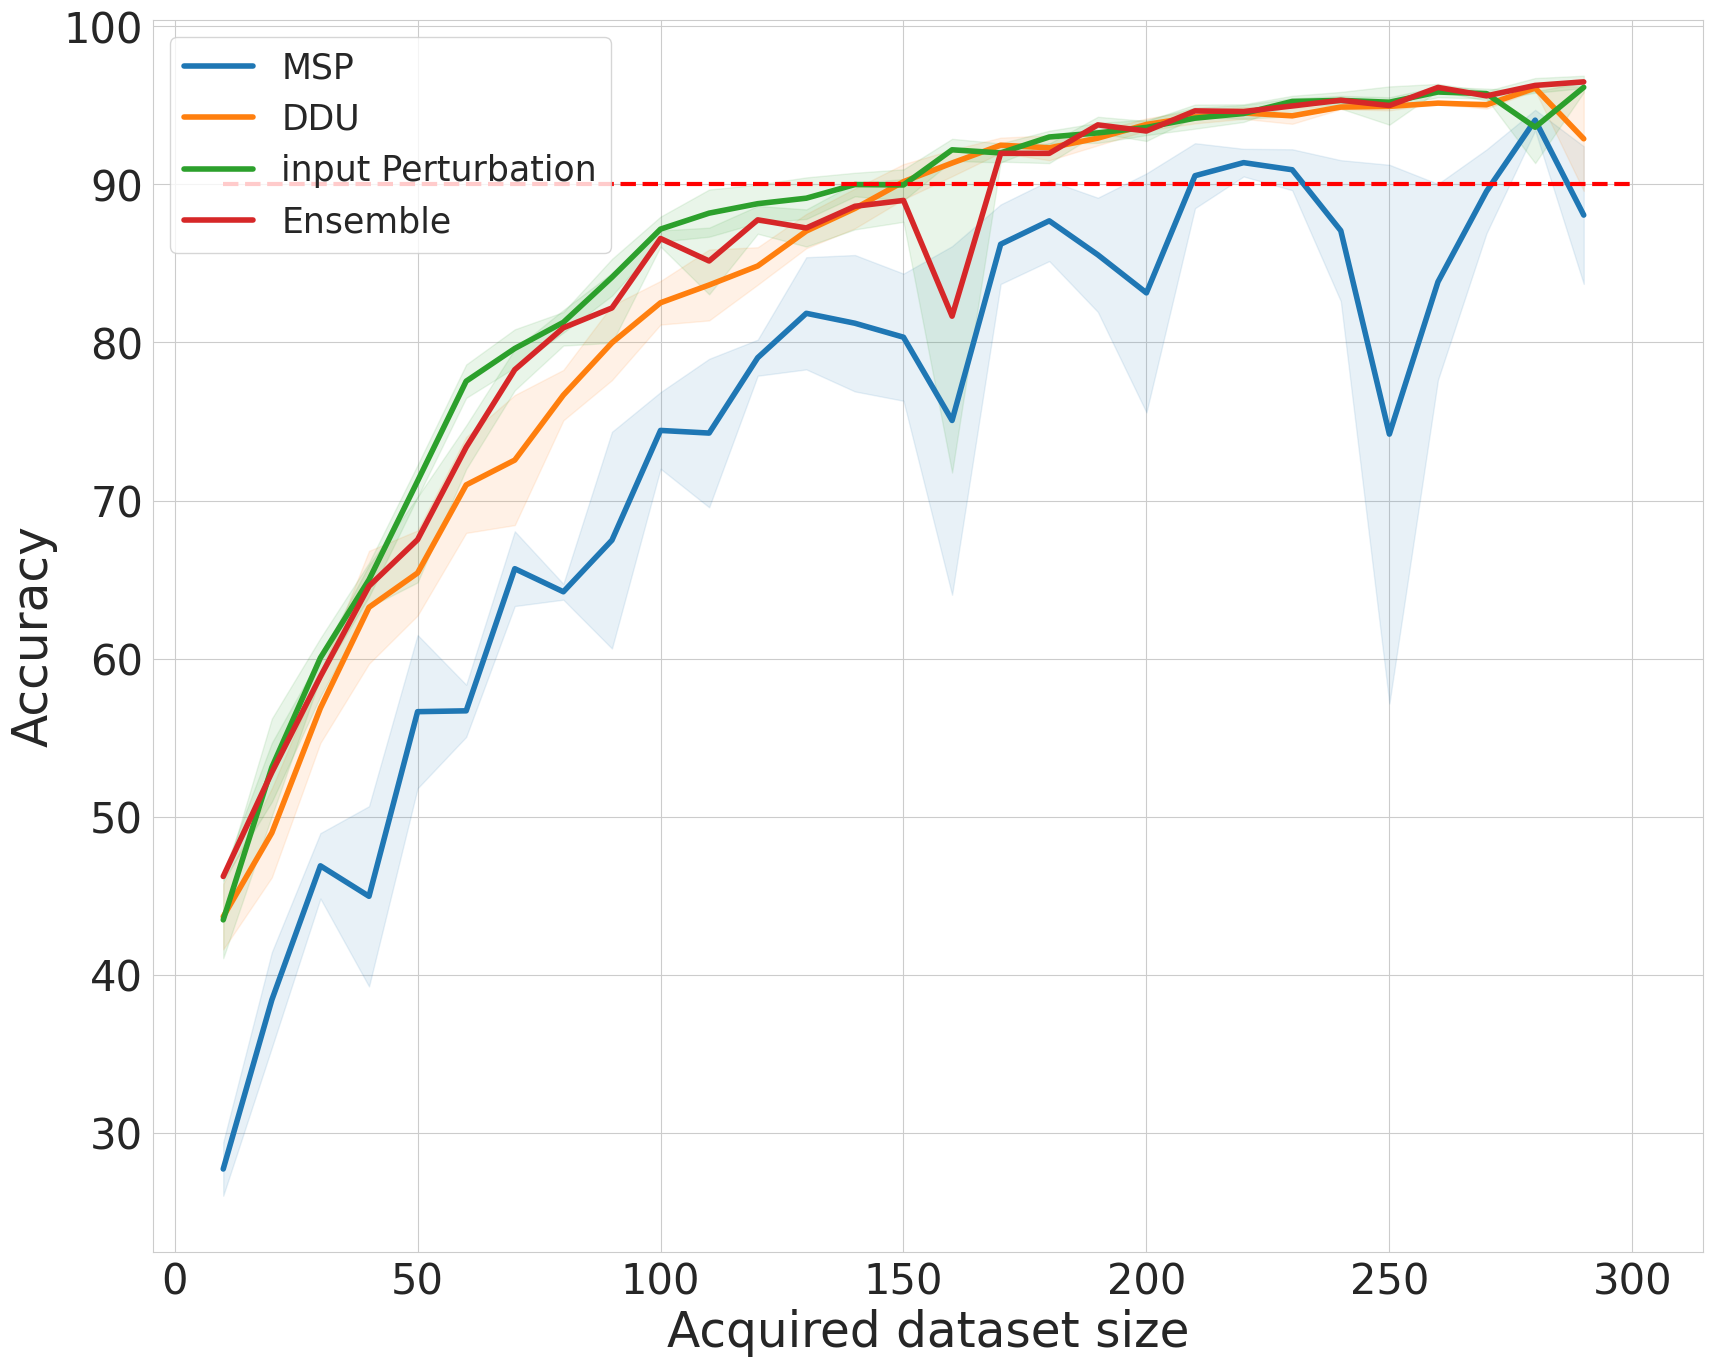
\includegraphics[width=0.75\linewidth]{assets/mnist_test_accuracy_active_learning.png}
    \caption{MNIST数据集,VGG16模型,主动学习任务上对比MSP,DDU,模型集成,基于输入扰动的改进等方法}
    \label{fig:active learning}
\end{figure}
本实验在 MNIST 数据集上训练 VGG16 模型,并将 MNIST 训练集分为两部分:一部分数据加入已标注的集合,另一部分作为候选池。初始时,已标注集合仅包含 20 个标注样本,模型首先在这些已标注样本上进行训练。随后,每次训练完成后,从候选池中选择模型不确定性最大的 10 个样本,并将其添加到已标注集合中,直到已标注集合的样本数量达到 300 个。在实验过程中,记录了每次训练完成后,模型在测试集上的准确率。实验结果如图 \ref{fig:active learning} 所示。

图 \ref{fig:active learning} 对比了四种模型不确定性建模方法:MSP,模型集成,DDU和本章提出的基于输入扰动的改进方法。图表展示了不同方法在主动学习任务中,随着数据集大小增加,MNIST 测试集准确率的变化趋势。横轴表示采集的数据集大小,纵轴表示 MNIST 测试集的准确率。实验结果表明,在相同的数据集大小下,基于输入扰动的改进方法在测试集上达到了最优的准确率,其次是模型集成方法,接着是 DDU 算法,最后是 MSP 方法。此结果表明,通过模型不确定性选择样本并将其加入已标注集合中,基于输入扰动的改进方法所选样本的价值最大,从而在建模模型不确定性的效果上,基于输入扰动的改进方法优于模型集成方法、DDU 算法和 MSP 方法。

\subsection{消融实验}
消融实验(Ablation Study)是机器学习和深度学习研究中常用的一种分析方法,用于评估模型中各个组件或设计选择的贡献及其对整体性能的影响。通过逐步移除(或替换)某些模块、特征或机制,观察模型性能的变化,从而帮助研究者理解每个部分的重要性和作用。在本节的实验中,本文对比了使用GDA和KDE\cite{davis2011remarks}(Kernel Density Estimation,核密度估计)两种不同的概率密度估计方式,并且对比了高为特征维度对模型不确定性建模的影响。

核密度估计是一种非参数化的概率密度估计方法,用于估计所给数据的概率密度函数(PDF)。给定一组独立同分布的样本点 $\{x_1, x_2, \ldots, x_n\}$,核密度估计的表达式如下:

\[
\hat{f}(x) = \frac{1}{n h} \sum_{i=1}^n K\left(\frac{x - x_i}{h}\right)
\]

其中:$x$ 是我们希望估计概率密度的点,$n$ 是样本数量,$h > 0$ 是带宽(平滑参数),控制核函数的扩展范围。$K(\cdot)$ 是核函数,通常满足以下性质: (1)非负性:$K(u) \geq 0, \forall u \in \mathbb{R}$,(2)积分为1:$\int_{-\infty}^\infty K(u) \, du = 1$,(3)对称性:$K(u) = K(-u)$。常用的核函数包括:高斯核(Gaussian Kernel),均匀核(Uniform Kernel),三角核(Triangle Kernel)。带宽 $h$ 是核密度估计中最重要的参数之一,如果 $h$ 过大,估计会过于平滑,丢失数据的细节。如果 $h$ 过小,估计会出现过拟合现象,导致噪声被放大。在本节的实验中,KDE选用的核函数是高斯核函数,其形式是\[K(u) = \frac{1}{\sqrt{2\pi}} e^{-\frac{u^2}{2}}\],带宽参数h通过交叉验证的方式选取最优值。

\begin{table}[h]
   \captionsetup{font=small, justification=centering}
    \centering
    \resizebox{\linewidth}{!}{
    \begin{tabular}{P{3cm} P{3cm} P{3cm} P{3cm} P{3cm}}
    \hline
    OOD Dataset & \makecell{AUROC/AUPRC\\(D=2048)} & \makecell{AUROC/AUPRC\\(D=1024)} & \makecell{AUROC/AUPRC\\(D=512)} & \makecell{AUROC/AUPRC\\(D=256)} \\
    \hline
    SVHN+GDA & \textbf{0.9179} / \textbf{0.9415} & \textbf{0.9322}/\textbf{0.9508} & 0.9310/0.9503 & 0.9320/0.9516 \\
    LSUN+GDA & \textbf{0.9239 }/ \textbf{0.9390} & \textbf{0.9353}/\textbf{0.9425} & \textbf{0.9363}/\textbf{0.9401} & \textbf{0.9332}/\textbf{0.9305} \\
    CIFAR100+GDA &\textbf{ 0.8888 }/ \textbf{0.9018}  & \textbf{0.9056}/\textbf{0.9131} & \textbf{0.9003}/\textbf{0.9066} & 0.8994/0.9021 \\
    MNIST+GDA &\textbf{ 0.9292 }/\textbf{0.9511}& \textbf{0.9439}/\textbf{0.9602} & 0.9342/0.9548 & 0.9308/0.9516 \\
    
    \hline
    SVHN+KDE & 0.8972/0.9168 & 0.9277/0.9496& \textbf{0.9320}/\textbf{0.9521} & \textbf{0.9422}/\textbf{0.9587} \\
    LSUN+KDE & 0.8957/0.9013 & 0.9199/0.9303 & 0.9218/0.9291 & 0.9278/0.9336 \\
    CIFAR100+KDE & 0.8380/0.8526 & 0.8837/0.9022 & 0.8905/0.9055 & \textbf{0.9013}/\textbf{0.9086} \\
    MNIST+KDE & 0.9151/0.9370 & 0.9370/0.9551& \textbf{0.9404}/\textbf{0.9570} & \textbf{0.9592}/\textbf{0.9596} \\
    \hline
    \end{tabular}
    }
    \caption{
    ResNet50+CIFAR10训练, 不同的概率密度建模方式GDA vs KDE, AUROC ($\uparrow$) and AUPRC ($\uparrow$), 选取的不同的特征维度:2048, 1024, 512和256.
    }
    \label{tag:GDAkde}
\end{table}





在本节实验中对比了所提取的高维特征在不同维度下,基于ResNet50模型在CIFAR10上训练后,使用GDA和KDE两种概率密度估计方法构建分布,在OOD检测任务中的性能。实验选取OOD检测任务间接评估模型不确定性的建模能力,选取了四个不同的OOD数据集(SVHN, LSUN, CIFAR100, MNIST),并以AUROC/AUPRC为报告指标,AUROC/AUPRC越高说明在OOD检测任务上的性能越好。实验结果见表格\ref{tag:GDAkde},并依据表格中的结果绘制折线图如图\ref{fig:GDAkde2}。
\begin{figure}[h]
    \captionsetup{font=small, justification=centering}
    \centering
    \includegraphics[width=0.9\linewidth]{assets/GDA_kde_dimension.png}
    \caption{ResNet50+CIFAR10训练, 不同的概率密度建模方式GDA vs KDE, AUROC ($\uparrow$) and AUPRC ($\uparrow$), 选取的不同的特征维度:2048, 1024, 512和256.}
    \label{fig:GDAkde2}
\end{figure}

从表格中可以看到,在不同维度(2048, 1024, 512, 256)下,使用GDA和KDE方法的表现有所不同。总体来看,在特征维度比较高时(D=2048),使用GDA构建概率分布的结果完全优于使用KDE构建概率分布,此时使用GDA构建概率分布在不同的OOD检测任务中都表现出更高的AUROC和AUPRC值,在较低维度(D=256)下,使用KDE构建概率分布的结果在大部分OOD检测任务上优于使用GDA构建概率分布,此时使用KDE构建概率分布在不同的OOD检测任务中表现出更高的AUROC和AUPRC值。在不同的OOD检测任务中,随着维度的减少,使用KDE构建概率分布所取得结果在逐渐变好,尤其是在256维时,KDE在大部分数据集上都取得了最好的结果。因此,选择适当的特征维度和不同的分布构建方法(GDA或KDE)对模型不确定性的建模至关重要。

由上述实验可以得出结论,特征维度较低时,使用KDE构建概率分布结果更好,但是特征维度高的时候,使用GDA构建概率分布效果更好。分析其中的原因,可能是因为在低维空间中,KDE得益于其非参数特性,不假设数据分布形状,能够充分利用每个点,有效地捕捉数据的局部结构和分布,但是随着数据维度的增加,样本数据密度变得更加稀疏,发生维度灾难(Curse of Dimensionality)\cite{murphy2012machine},经验分布无法捕捉到真实分布的结构, KDE的表现会下降。在高维数据中GDA具有数据符合高斯分布的先验假设,每个高斯分布可以通过调整均值、方差和权重来捕捉数据的分布,在高维空间中通过依赖协方差矩阵建模维度间的关系,能够适当捕捉相关性,不会受到高维稀疏性的强烈影响。而且,GDA通过参数(均值、协方差矩阵和权重)来定义分布,相比于KDE,避免了KDE的计算瓶颈。 


\section{本章小结}

传统的模型集成方法或贝叶斯神经网络在不确定性建模上虽然效果较好,但由于计算和存储开销大,单一确定性的建模方法正逐渐受到关注。为高效建模不确定性,本章针对基于高维特征概率密度估计的不确定性建模方法展开研究。DDU算法作为其中的一个最新代表,通过高斯判别分析模型在高维特征空间上构建概率密度分布并计算概率密度来度量不确定性,然而,DDU算法在某些复杂网络架构和数据集上表现相对集成方法在不确定性建模的效果上仍有差距。

本章通过分析神经网络的梯度空间,探讨了分布内样本和分布外样本在梯度响应上的差异性。实验结果表明,分布外样本在梯度响应图上的梯度较大,这一现象表明梯度信息与模型不确定性密切相关。基于这一观察,本章提出了基于输入扰动的改进方法,通过对输入样本施加与梯度响应相关的微小扰动,进一步放大了分布内样本和分布外样本在概率分布上的差异。输入扰动的引入能够使得域内样本和域外样本在经过高斯判别分析模型建模的高维特征空间中表现出更为显著的分布差异,从而在不确定性度量中更好地区分异常样本。这一方法可以有效地改善DDU算法在不同数据集上的不确定性建模能力,尤其是在OOD检测、误分类样本识别和对抗样本检测等任务中表现出色。

在理论分析方面,本章通过推导和分析概率密度关于输入的梯度性质,揭示了输入扰动对模型不确定性度量的影响。输入扰动沿着梯度方向进行调整,会使得分布外样本的特征向量远离类别均值,从而使得其在多维概率分布上的概率密度值下降,进一步增强了模型对不确定性的敏感性。通过这种方式,输入扰动有效提高了不确定性建模的能力,尤其是在处理OOD样本时,能够明显增加OOD样本与InD样本在不确定性分布上的差异。

此外,通过对比不同的概率密度估计方法(如GDA与KDE)和特征维度的影响,本章进一步探讨了在特定条件下选择合适的建模方法对于不确定性建模性能的重要性。在低维特征空间中,KDE能够更好地捕捉数据的局部结构,而在高维特征空间中,GDA则展现出了更强的建模能力,尤其是在应对高维稀疏性和维度灾难时,GDA的表现更为稳健。

综上所述,本章提出的基于输入扰动的改进策略显著提升了基于高维特征概率密度估计的不确定性建模效果,并在多个任务中展示了其优越的性能。这一方法可以更准确高效地建模不确定性,为提高深度学习模型在高风险领域的应用提供了新的思路和技术支持。




\chapter{基于辅助损失函数联合训练的改进策略}
\section{引言}
神经网络的不确定性是对其预测结果置信度的度量,不确定性分析可以帮助模型提供更可靠的决策依据。本文研究了基于高维特征概率密度估计的模型不确定性建模方法,该方法无需训练多个模型或多次推理,从而提高了不确定性的建模效率。为了进一步提升模型不确定性建模效果,第三章提出了一种基于输入扰动的策略。该策略通过引入与梯度响应相关的扰动,显著增大了分布内样本和分布外样本在概率分布空间中的差异,从而增强了模型对不确定性量化的区分能力。值得注意的是,该方法无需修改已训练的神经网络架构,能够直接应用于现有模型。

尽管基于输入扰动的策略取得了一定成效,但在特征空间优化方面本文的不确定性建模方法仍有改进空间。由于未改变训练过程,类内样本的紧密性和类间样本的可分性仍有待提升。基于高维特征概率密度估计的模型不确定性建模受特征空间结构的影响,如果能够在训练过程中优化特征空间结构,使得类内样本更紧密、类间样本更可分,则可以显著提高不确定性建模的精度和鲁棒性。

因此,本章将探讨如何通过改变训练方式,进一步优化高维特征空间结构。在深度学习应用中,有效对高维特征进行概率密度建模是一个核心挑战。通过建模这些高维特征的概率分布,不仅可以有效捕捉数据分布特征,还能解决异常检测、不确定性量化和生成建模等问题。传统的分类方法中,交叉熵损失函数(Cross-Entropy Loss)广泛应用于监督学习任务,旨在最小化预测类别与真实类别之间的差异。然而,在高维特征空间中,类别间的重叠和样本分布的稀疏性使得直接进行概率密度建模变得复杂。度量学习作为优化特征空间表示的有效方法,提供了解决这一问题的可能性。

度量学习\cite{kaya2019deep}\cite{kulis2013metric}\cite{yang2006distance}是机器学习中的一个重要分支,旨在学习适用于特定任务的距离度量。该方法通常用于度量特征空间中样本之间的相似度或差异度,广泛应用于人脸识别、图像检索、推荐系统和自然语言处理等领域。度量学习的核心目标是学习一个距离函数,使得相似样本在特征空间中接近,不相似样本远离。与传统的分类或回归任务不同,度量学习通过优化样本之间的相对距离关系,而非直接优化类别预测,从而间接提高任务性能。度量学习中的距离函数通常包括欧几里得距离、马氏距离和余弦相似度等。根据学习方式的不同,度量学习方法可以分为基于距离函数的学习算法和基于相似度/差异度的学习算法。常见的度量学习算法包括Siamese网络\cite{bromley1994signature}、三元组网络\cite{schroff2015facenet}、对比损失\cite{hadsell2006dimensionality}等。

本文提出了一种通过神经网络训练引入度量学习约束的方法,使得高维特征空间的样本分布更加适合高斯判别分析(GDA)模型进行概率密度建模。特征空间的性质对不确定性建模效果至关重要,度量学习通过优化特征表示,使相似样本更加紧密、不相似样本更远离,从而有效减少高维空间中不确定性建模的复杂性。此外,度量学习有助于提高特征分布的聚集性和可分性,从而提高概率密度估计的精度。本章设计了一种新的辅助损失函数(Auxiliary Loss),与交叉熵损失函数共同训练(如图\ref{tag:模型结构图2}所示),实现了特征空间的类内紧密性和类间可分性,从而提升了基于高维特征的概率密度建模神经网络不确定性的效果,并在OOD检测等任务上进行了验证。

此外,随着深度学习的广泛应用,特征降维技术已成为高效数据处理和分析的重要工具。由于神经网络提取的高维特征可能维度过高(如ResNet50提取的特征维度为2048维),这可能导致维度灾难\cite{murphy2012machine}、计算复杂度过高以及过拟合等问题。为了有效进行概率密度建模和计算,本章研究了降维技术的应用,提出采用主成分分析(PCA,Principal Component Analysis)作为降维方法,旨在减少GDA对高维特征建模时的存储空间需求。PCA是一种广泛应用于数据压缩、特征选择和数据可视化等领域的降维技术。本章将PCA用于高维特征降维,并在降维后的特征上重新建立GDA模型。通过理论分析PCA降维前后的时间复杂度和空间复杂度,并通过实验验证,GDA结合PCA降维能够显著减少存储空间需求并提高建模效率。
\section{主要方法}
\subsection{辅助损失函数联合训练}

首先介绍下高维特征空间上的类内紧密性和类间可分性,如图\ref{interintra}。

\begin{figure}[h]
    \centering
    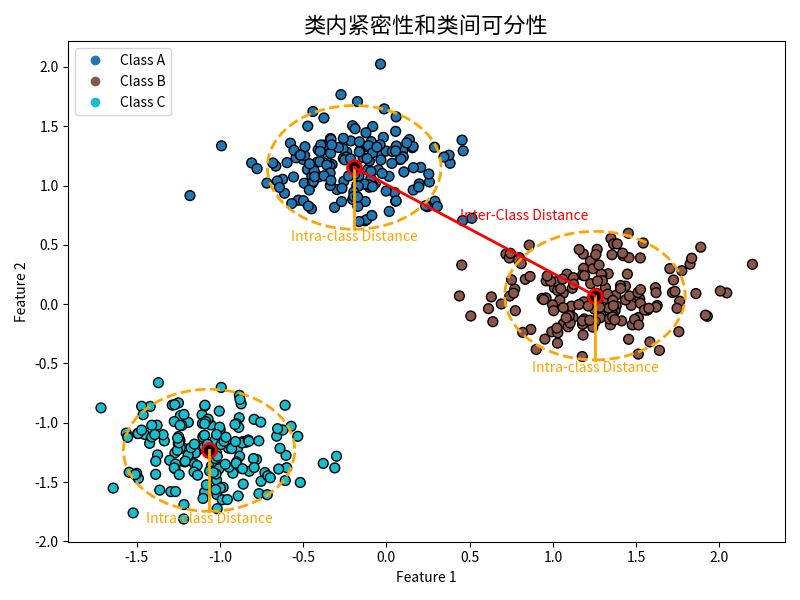
\includegraphics[width=1.\linewidth]{assets/inter-intra.png}
    \caption{类内紧密性和类间可分性}
    \label{interintra}
\end{figure}

\textbf{类内紧密性}(Intra-class Compactness)指的是同一类别的样本在特征空间中分布得多么紧密,提升类内紧密性的目的是使同一类别的样本在特征空间中更接近。高类内紧密性意味着表示同一类别的样本在特征空间中聚集在一起,样本的特征能够很好地描述同一类别的特性,减少了同一类别样本之间的差异。 \textbf{类间可分性}(Inter-class Separability)指的是不同类别的样本在特征空间中的分离程度,提升类间可分性的目的是使不同类别的样本在特征空间中相距更远。高类间可分性意味着不同类别在特征空间中有更明显的分隔,类别之间有明显的边界,这有助于分类器在决策边界上更好地区分不同类别。理想状态下,在特征空间中,同一类别的样本应该分布紧密(即高类内紧密性),而不同类别的样本之间应该相距较远(即高类间可分性)。但是当数据维度增加或样本类别分布复杂时,这两者可能会受到限制。例如,噪声数据会降低类内紧密性,而类别间的相似性会降低类间可分性。通过优化类内紧密性和类间可分性,分类模型能够更高效地学习特征表示,提高分类的准确性。



CenterLoss\cite{wen2016discriminative}是一种用于深度学习中的损失函数,主要应用于人脸识别和特征嵌入学习等任务。其核心目标是通过最小化同一类别样本特征向量与该类中心之间的欧几里得距离,优化特征空间中的类内距离,从而提高模型的区分能力CenterLoss定义为:

\[
L_{\text{center}} = \frac{1}{2N} \sum_{i=1}^{N} \| f(x_i) - c_{y_i} \|^2
\]

其中,\( f(x_i) \) 表示输入样本 \( x_i \) 的特征表示,\( c_{y_i} \) 为类别 \( y_i \) 的类别中心,\(\|\cdot\|\) 是欧几里得距离,\( N \) 为样本数量。通过这种方式,CenterLoss 使得同类别的样本在特征空间中更加集中,从而提升分类性能和类别区分能力。在实际应用中,CenterLoss 通常与 Softmax 损失函数结合使用,进一步增强模型的分类效果通,过联合优化这两个损失,网络不仅能够学习到更精确的分类决策,还能够使得特征空间中的样本更加紧密。。

从CenterLoss的定义上看,仅仅包含类内紧密性的损失函数,为了提高特征空间上的类间可分性,可以考虑在其原始公式的分母上引入一些提高类间可分性的项。这种改进可以通过设计一个新的权重项,使得在计算类间距离时,能够更强调类别间的分隔性,从而增强不同类别特征的区分度。为了提高类间可分性,本文提出了一个新的辅助损失函数,在其中加入与类别间距离相关的项,从而惩罚相近类别的样本特征,使得不同类别在特征空间上更加远离。将分母中加入一个与类别中心间距相关的因子来增强类间可分性,新的损失函数公式具体如下:

\[
\text{AuxLoss} = \frac{1}{2} \sum_{i=1}^m \frac{\|x_i - C_{y_i}\|_2^2}{\sum_{j=1, j \neq y_i}^{m} \|C_{y_i} - C_j\|_2^2 + \delta}.
\],

这里 \( C \) 是类别数,\( c_k \) 是类别 \( k \) 的中心,\( \delta \) 是一个小常数,用于数值稳定性,防止除零错误。

通过在分母中引入$\sum_{j=1, j \neq y_i}^{m} \|C_{y_i} - C_j\|_2^2$,让距离较远的类别中心在优化过程中贡献更少的惩罚项,反之,距离较近的类别中心将会对损失值产生更大的影响。这种方式鼓励类别间的分隔,使得样本的特征在同一类别内紧密、而在不同类别间具有更大的间隔。随着训练的进行,样本在特征空间中的分布会越来越偏向于形成更加清晰的类别分隔。通过调整类别间距的方式,可以有效减少类间重叠,从而增强模型对不同类别的区分能力。

这种新提出的AuxLoss可以作为辅助损失加入到交叉熵损失函数中(如图\ref{tag:模型结构图2},进一步强化特征的聚合与类间分隔。在训练过程中,原本的交叉熵损失负责指导分类准确性,而改进后的AuxLoss则帮助网络在优化特征表示时,通过引入类别中心之间的间距来进一步优化类别分离的效果,更好地考虑到类别之间的相对距离。


\begin{figure}[h]
    \centering
    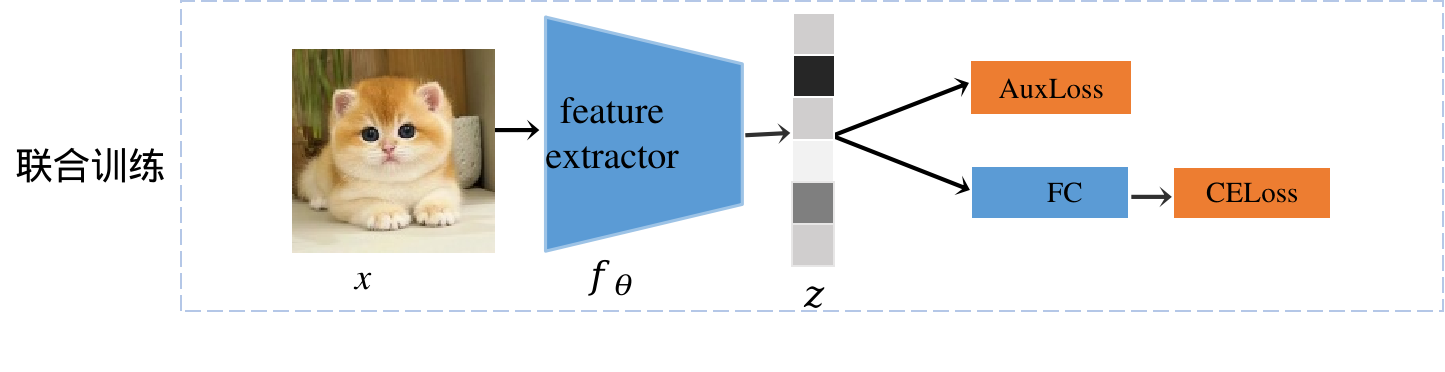
\includegraphics[width=1.\linewidth]{assets/structure2.png}
    \caption{基于高维特征概率密度建模的模型不确定性}
    \label{tag:模型结构图2}
\end{figure}


CrossEntropyLoss和AuxLoss联合训练的公式如下:
\begin{equation}
    L = L_s+\lambda * L_x
\end{equation}

其中,$L_s$是CrossEntropyLoss,公式如下:

\begin{equation}
    L_s= - \sum_{i=1}^C y_i \log\left(\frac{\exp(z_i)}{\sum_{j=1}^C \exp(z_j)}\right)
\end{equation}

$L_x$是修正后的AuxLoss,公式如下:
\begin{equation}
    L_x = \frac{1}{2}\sum_{i=1}^{m} \frac{\Vert x_i-C_{y_i}\Vert_2^2}{\sum_{j=1,j\neq y_i}^{m}\Vert C_i-C_j\Vert_2^2+\delta}
\end{equation}

上述AuxLoss,分子项通过特征向量与其对应类别中心距离的最小化保证类内紧密性,分母项通过不同类别中心的距离最大化来保证类间可分性。在具体实现时,类别中心是基于正态分布随机初始化的,它会作为模型的一部分进行学习和优化。类别中心会随着模型的训练过程而更新,类别中心作为模型参数的一部分,损失函数反向传播时,PyTorch框架通过优化器自动更新类别中心的值。关于上述AuxLoss的损失函数对参数类中心的求导,有以下的结论。

\textbf{性质4.1:}
给定的损失函数如下:

\[
L_x = \frac{1}{2} \sum_{i=1}^m \frac{\|x_i - C_{y_i}\|_2^2}{\sum_{j=1, j \neq y_i}^{m} \|C_{y_i} - C_j\|_2^2 + \delta}.
\]
其中:
\( x_i \) 是第 \( i \) 个样本的输入,\( y_i \) 是第 \( i \) 个样本的类别标签,\( C_k \) 是类别 \( k \) 的特征中心,\( \delta \) 是一个正的平滑常数。则关于每个类中心的梯度为:


当 \( j = y_i \) 时:
\[
\frac{\partial L_x}{\partial C_j} =  \sum_{i: y_i = j} \left( \frac{- (x_i - C_j)}{B_i} - \frac{A_i}{B_i^2} \sum_{k=1, k \neq j}^m  (C_j - C_k) \right).
\]

当 \( j \neq y_i \) 时:
\[
\frac{\partial L_x}{\partial C_j} = -\sum_{i: y_i \neq j} \left( \frac{A_i}{B_i^2} (C_{y_i} - C_j) \right).
\]


\textbf{证明}:
需要对损失函数求关于 \( C_j \) 的梯度。为了方便,将损失函数记为:

\[
L_x = \frac{1}{2} \sum_{i=1}^m \frac{A_i}{B_i},
\]

其中:
\[
A_i = \|x_i - C_{y_i}\|_2^2, \quad B_i = \sum_{j=1, j \neq y_i}^m \|C_{y_i} - C_j\|_2^2 + \delta.
\]

\[
\frac{\partial L_x}{\partial C_j} = \frac{1}{2} \sum_{i=1}^m \frac{\partial}{\partial C_j} \left( \frac{A_i}{B_i} \right).
\]

使用商的求导法则:
\[
\frac{\partial}{\partial C_j} \left( \frac{A_i}{B_i} \right) = \frac{1}{B_i} \frac{\partial A_i}{\partial C_j} - \frac{A_i}{B_i^2} \frac{\partial B_i}{\partial C_j}.
\]

因此,梯度可以分解为两部分:
\[
\frac{\partial L_x}{\partial C_j} = \frac{1}{2} \sum_{i=1}^m \left( \frac{1}{B_i} \frac{\partial A_i}{\partial C_j} - \frac{A_i}{B_i^2} \frac{\partial B_i}{\partial C_j} \right).
\]

1.求 \( \frac{\partial A_i}{\partial C_j} \):

当 \( j = y_i \) 时:
\[
A_i = \|x_i - C_{y_i}\|_2^2, \quad \frac{\partial A_i}{\partial C_j} = \frac{\partial}{\partial C_j} \|x_i - C_j\|_2^2 = -2 (x_i - C_j).
\]

当 \( j \neq y_i \) 时:
\[
A_i \text{ 与 } C_j \text{ 无关,因此 } \frac{\partial A_i}{\partial C_j} = 0.
\]

2.求 \( \frac{\partial B_i}{\partial C_j} \)
\[
B_i = \sum_{k=1, k \neq y_i}^m \|C_{y_i} - C_k\|_2^2 + \delta.
\]

当 \( j = y_i \) 时:
\[
\frac{\partial B_i}{\partial C_j} = \frac{\partial}{\partial C_j} \sum_{k=1, k \neq y_i}^m \|C_j - C_k\|_2^2 = \sum_{k=1, k \neq y_i}^m 2 (C_j - C_k).
\]

当 \( j \neq y_i \) 时:
\[
\frac{\partial B_i}{\partial C_j} = \frac{\partial}{\partial C_j} \|C_{y_i} - C_j\|_2^2 = -2 (C_{y_i} - C_j).
\]


综合梯度,将以上结果代入:

当 \( j = y_i \) 时:
\[
\frac{\partial L_x}{\partial C_j} =  \sum_{i: y_i = j} \left( \frac{- (x_i - C_j)}{B_i} - \frac{A_i}{B_i^2} \sum_{k=1, k \neq j}^m  (C_j - C_k) \right).
\]

当 \( j \neq y_i \) 时:
\[
\frac{\partial L_x}{\partial C_j} = -\sum_{i: y_i \neq j} \left( \frac{A_i}{B_i^2} (C_{y_i} - C_j) \right).
\]


下面,通过可视化高维特征空间,定性分析加入辅助损失函数联合训练对高维特征空间的影响。在CIFAR10数据集上训练ResNet50网络,分别使用原始交叉熵损失函数训练网络和使用交叉熵损失函数加辅助损失函数联合训练的方法。
\begin{table}[H]
\captionsetup{font=small, justification=centering} % 设置标题字体大小与对齐方式
\centering
\begin{tabular}{|c|c|c|}
\hline
\textbf{} & \textbf{CELoss} & \textbf{CELoss+AuxLoss} \\ \hline % 使表头加粗
\begin{minipage}{0.1\textwidth} \centering VGG \end{minipage} & 
\begin{minipage}{0.45\textwidth} \centering 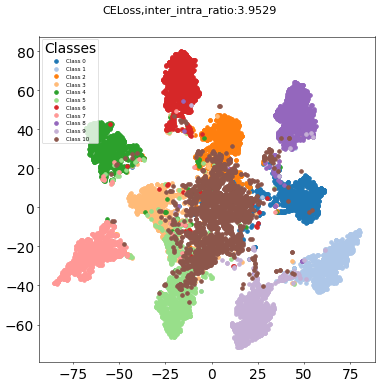
\includegraphics[width=\textwidth]{assets/vgg16_tsne_feature.png} \end{minipage} & 
\begin{minipage}{0.45\textwidth} \centering 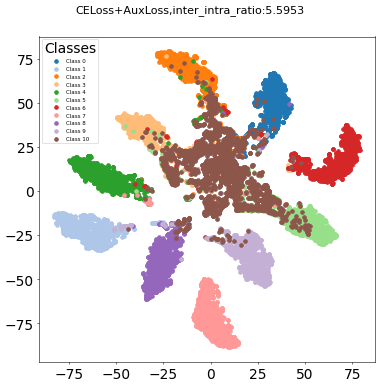
\includegraphics[width=\textwidth]{assets/vgg16_tsne_feature_c.png} \end{minipage} \\ \hline
\begin{minipage}{0.1\textwidth} \centering ResNet \end{minipage} & 
\begin{minipage}{0.45\textwidth} \centering 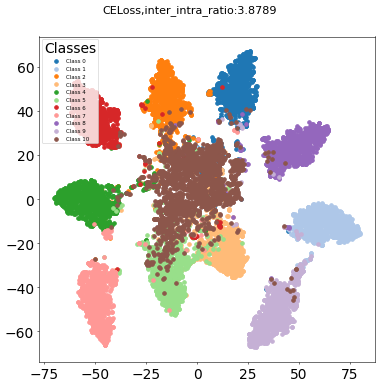
\includegraphics[width=\textwidth]{assets/resnet50_tsne_feature.png} \end{minipage} & 
\begin{minipage}{0.45\textwidth} \centering 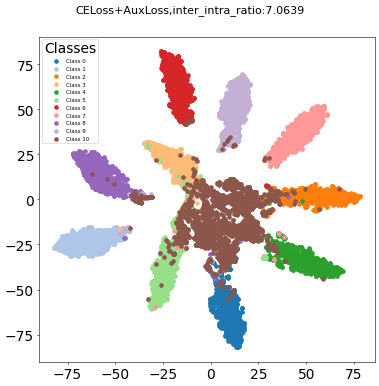
\includegraphics[width=\textwidth]{assets/resnet50_tsne_feature_c.png} \end{minipage} \\ \hline
\begin{minipage}{0.1\textwidth} \centering ViT \end{minipage} & 
\begin{minipage}{0.45\textwidth} \centering 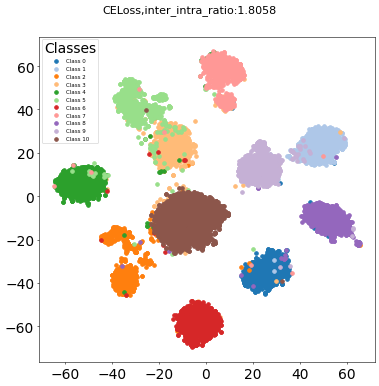
\includegraphics[width=\textwidth]{assets/vit_tsne_feature.png} \end{minipage} & 
\begin{minipage}{0.45\textwidth} \centering 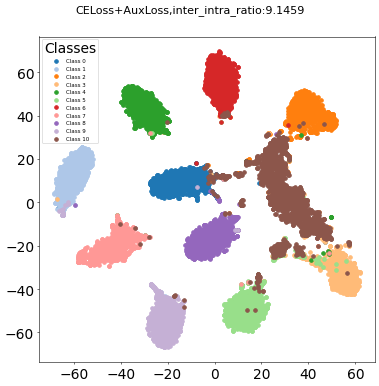
\includegraphics[width=\textwidth]{assets/vit_tsne_feature_c.png} \end{minipage} \\ \hline
\end{tabular}
\caption{在CIFAR10数据集上训练不同的模型(VGG16、ResNet50、ViT),测试集上特征空间的t-SNE可视化, 左侧为交叉熵损失函数单独训练的模型,右侧为交叉熵损失函数与辅助损失函数联合训练的模型。}
\label{cifar10-tsne}
\end{table}

训练得到的高维特征难以直接进行可视化分析,所以本文使用t-SNE(t-Distributed Stochastic Neighbor Embedding)\cite{van2008visualizing}方法先对高维特征进行降维到2维空间上。t-SNE是一种常用的降维方法,能够将高维数据映射到二维或三维空间中,同时保持样本间的相对距离。通过在降维后的特征空间中可视化数据点,可以直观地看到类内样本的聚集情况和类别间的分离情况。
t-SNE可视化高维特征空间结果如图\ref{cifar10-tsne}。


左图展示了仅使用交叉熵损失函数训练的结果。从图中可以看出,不同类别的数据点(用不同颜色表示)在特征空间中有一定的分离,但仍然存在一些重叠和模糊的区域。这表明模型在某些类别上的区分能力有限。右图展示了使用交叉熵损失函数和辅助损失函数联合训练的结果。从图中可以看出,不同类别的数据点在特征空间中的分离更加明显,重叠和模糊的区域大大减少。这表明模型在区分不同类别时的能力得到了显著提升。图上Inter\_intra\_ratio是类间距离比类内距离,从图中可以看到右侧的普遍较大,说明右侧使用辅助损失函数联合训练的模型,抽取的高维特征类间可分性和类内紧凑性更好。由此得出结论:辅助损失函数的加入使得模型在特征空间中的表示更加清晰和分离,从而提高了分类的准确性。加入辅助损失函数联合训练能提高模型在特征空间中的区分能力,从而提升分类性能,并更容易在高维特征空间上进行概率分布建模。


为了定量地分析加入辅助损失函数联合训练后,特征空间上类内紧密性和类间可分性的变化,本章使用类内距离 (Intra-class Distances)、Davies-Bouldin 指数 (Davies-Bouldin Index,DBI)\cite{davies1979cluster}、类间距离(Inter-class Distances)、Fisher 比率 (Fisher Ratio) 和 轮廓系数 (Silhouette Coefficient)\cite{rousseeuw1987silhouettes}等几个指标度量。在测试集上计算这几个指标,结果见表\ref{feature_analysis}。以下是关于 类内距离、、类间距离、Fisher 比率  和 轮廓系数 的详细介绍及公式。

类内距离衡量同一类别中所有样本对之间的平均距离,反映同一类样本的紧密程度。
\[
D_{\text{intra}}(C_k) = \frac{1}{|C_k|^2} \sum_{i \in C_k} \sum_{j \in C_k} d(x_i, x_j)
\]
其中:$C_k$是类 $k$ 中的样本集合, $|C_k|$是类 $k$ 的样本数量 $d(x_i, x_j)$是样本 $x_i$ 和 $x_j$ 之间的距离。

类间距离 用于衡量不同聚类之间的分离程度,通常计算聚类中心之间的距离。

\[
D_{inter} = \sum_{i=1}^{C} N_i (\mu_i - \mu)^2
\]

其中:  \( C \) 是类别的数量,   \( N_i \) 是第 \( i \) 类的样本数量,  \( \mu_i \) 是第 \( i \) 类的均值, \( \mu \) 是所有样本的全局均值。该公式表示各个类别均值 \( \mu_i \) 与全局均值 \( \mu \) 之间的加权距离,权重为各类别的样本数量 \( N_i \)。

Davies-Bouldin 指数衡量聚类的质量,综合考虑了类内紧密性和类间分离性,值越小表示聚类效果越好。
\[
DBI = \frac{1}{K} \sum_{k=1}^K \max_{j \neq k} \frac{S_k + S_j}{d_{kj}}
\]
其中:$K$是类别数;$S_k$是类 $k$ 的类内散布性(如类内平均距离);$d_{kj}$是聚类 $k$ 和聚类 $j$ 的中心之间的距离。


Fisher 比率用于衡量不同类别之间的可分性,通常定义为类间散布和类内散布的比值。其公式为:

\[
F = \frac{S_B}{S_W}
\]

其中, \( S_B \) 表示类间散布,  \( S_W \) 表示类内散布。
类间散布 \( S_B \) 定义为:$S_B = \sum_{i=1}^C N_i (\mu_i - \mu)^2$,其中:  \( C \) 是类别数量,   \( N_i \) 是第 \( i \) 类的样本数量,   \( \mu_i \) 是第 \( i \) 类样本的均值,  \( \mu \) 是所有样本的全局均值。类内散布 \( S_W \) 定义为:$S_W = \sum_{i=1}^C \sum_{x \in \mathcal{D}_i} (x - \mu_i)^2 $
其中:  \( \mathcal{D}_i \) 是第 \( i \) 类的样本集合,  \( x \) 是样本点。当 \( S_B \) 较大、\( S_W \) 较小时,Fisher 比率趋向较大值,表示特征具有较强的区分能力。  当 \( S_B \) 和 \( S_W \) 相近时,Fisher 比率较小,表示该特征对类别区分的贡献较弱。


轮廓系数 用于评估聚类的紧密性和分离性,取值范围为 $[-1, 1]$。值越接近 $1$ 表示聚类效果越好。单个样本 $i$ 的轮廓系数定义为:
\[
s(i) = \frac{b(i) - a(i)}{\max(a(i), b(i))}
\]

其中:$a(i)$是样本 $i$ 到其所在聚类中其他样本的平均距离(类内距离);$b(i)$是样本 $i$ 到最邻近的其他聚类的所有样本的平均距离(类间距离)。总体轮廓系数为所有样本轮廓系数的平均值:
\[
S = \frac{1}{N} \sum_{i=1}^N s(i)
\]


\begin{table}[H]
\captionsetup{font=small, justification=centering}
\centering
\renewcommand{\arraystretch}{1.2} % 调整行间距
\setlength{\tabcolsep}{6pt} % 调整列间距
\resizebox{\textwidth}{!}{ % 缩放表格以适应页面宽度
\begin{tabular}{c c c c c c c}
\hline
\textbf{训练策略} & \textbf{Model} & \textbf{IntraClassDistance($\downarrow$)} & \textbf{DaviesBouldinIndexs($\downarrow$)} & \textbf{InterClassDistances($\uparrow$)} & \textbf{FisherRatios($\uparrow$)} & \textbf{SilhouetteCoefficients($\uparrow$)} \\ 
\hline
\multirow{3}{*}{CE Loss} 
& VGG16 & 1.8466 & 0.3687   & 11.4856 & 13.3970 & 0.7520 \\ 
& ResNet50 & \textbf{1.5544}  & 0.3775  & 9.4415 & 13.8453 & 0.7408 \\ 
& VIT & 5.6329 & 0.8430 & 14.7451 & 3.6832 & 0.5080 \\ 
\hline
\multirow{3}{*}{联合训练} 
& VGG16 & \textbf{0.7806}  & \textbf{0.0981} & \textbf{19.4277} & \textbf{136.1505} & \textbf{0.9360} \\ 
& ResNet50 & 3.0138  & \textbf{0.1952} & \textbf{34.6706} & \textbf{44.3006} & \textbf{0.8675} \\ 
& VIT & \textbf{2.3761} & \textbf{0.1937} & \textbf{30.1605} & \textbf{89.0348} & \textbf{0.8698} \\ 
\hline
\end{tabular}
}
\caption{对比加入辅助损失函数前后特征空间类内紧密性和类间可分性的变化}
\label{feature_analysis}
\end{table}

在实验结果中,加入辅助损失函数后,所有模型在特征空间中的类内紧密性和类间可分性均有显著提升。从类内距离来看,使用辅助损失函数联合训练的模型相比于仅使用交叉熵损失函数能够显著降低类内样本之间的距离,同时Davies-Bouldin指数也得到了明显改善,这表明类内的紧密性得到了增强。类间距离和Fisher比率则呈现出明显的上升,表明类别之间的间隔增大,模型对不同类别的区分度得到了增强。轮廓系数也有所提高,进一步验证了样本在特征空间中的分离效果。

综上所述,加入辅助损失函数能够有效提高模型在特征空间中的类内紧密性和类间可分性。这一改进不仅优化了样本的聚合效果,还增强了类别之间的分隔性,提高了模型在分类任务中的表现,使用高斯判别分析模型能够更好地在特征空间上建模分布。


\subsection{高维特征降维}

高维特征概率密度建模旨在对高维数据的分布进行概率密度估计,通常用于描述样本的分布特征。但是随着数据维度的增加(如ResNet50模型提取的高维特征为2048维),高维数据可能带来一些问题,如维度灾难、计算复杂度和过拟合风险。首先,随着特征维度的增加,数据点之间的距离逐渐增大,导致数据变得稀疏,如何有效地建模这种稀疏性,成为高维数据分析中的重要挑战。在高维空间中,原来的距离度量(如欧氏距离)逐渐失效,使得有效的概率密度建模变得更加困难。其次,随着维度的增加,计算复杂度急剧上升,尤其是对于基于密度估计的非参数方法(如核密度估计、高斯判别分析模型),需要大量计算资源,并且容易受到噪声的干扰。最后,高维数据的稀疏性使得模型容易过拟合训练数据,捕捉到噪声而非数据的真实结构,从而导致模型泛化能力下降。为了解决高维数据存在的上述问题,主要的思路是使用机器学习中的降维技术。


\begin{figure}[h]
    \centering
    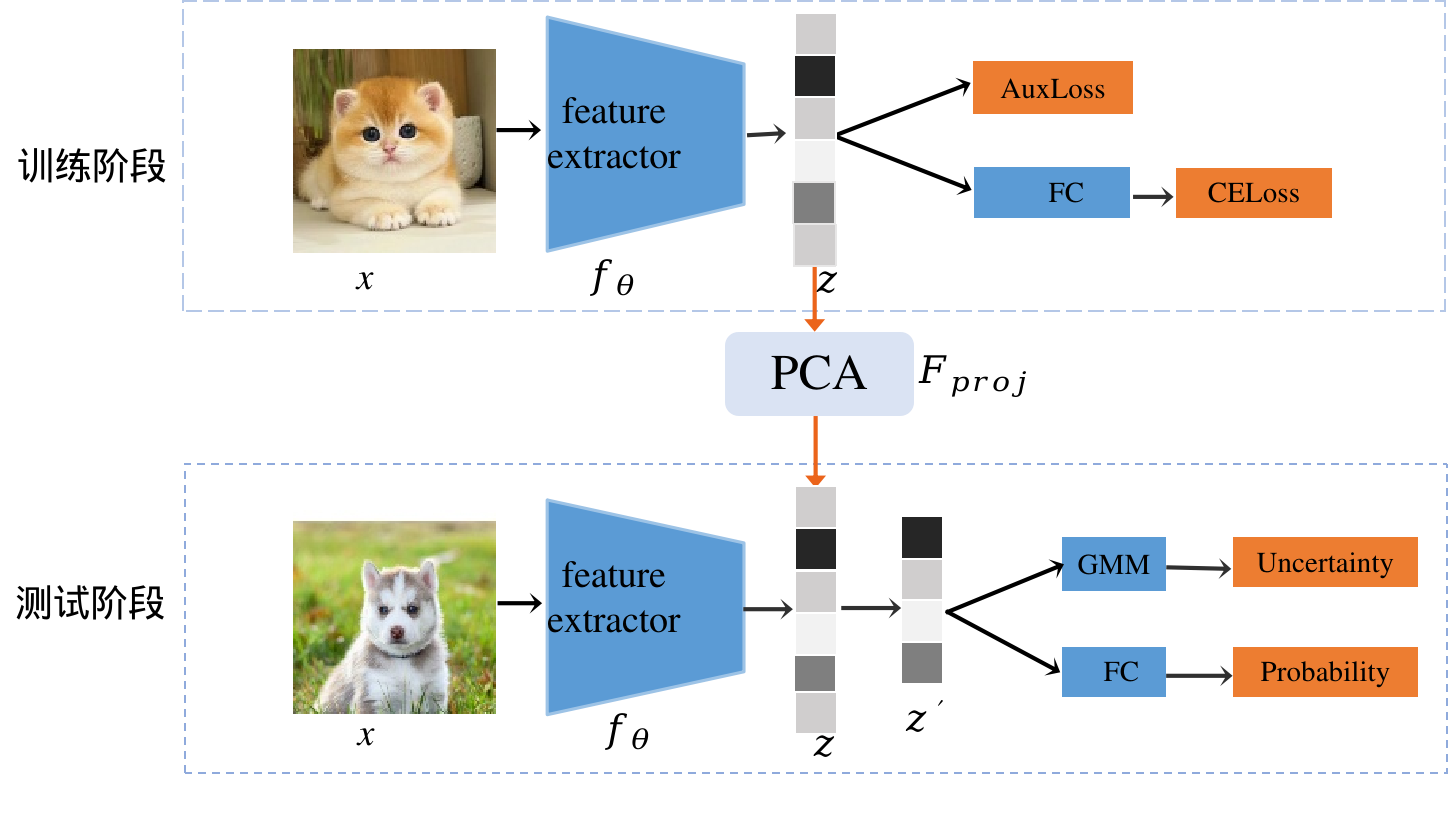
\includegraphics[width=1.\linewidth]{assets/structure3.png}
    \caption{基于高维特征概率密度建模的模型不确定性}
    \label{tag:模型结构图3}
\end{figure}


PCA(Principal Component Analysis,主成分分析)是一种常见的降维技术,用于将高维数据转换为低维数据,同时尽可能保留数据的主要特征信息。PCA通过找到数据中方差最大的方向,将数据投影到这些方向上,从而达到降维的目的,如图\ref{tag:pca}所示。PCA应用到高维数据上,通过减少数据的维度,可以显著降低计算复杂度。在高维数据处理中,PCA常用于减少数据维度,去除冗余信息,使得后续的机器学习模型更加高效。通过降维,PCA可以去除一些噪声和无关的特征,帮助减轻过拟合问题,提高模型的泛化能力。 PCA算法主要步骤如下\cite{jolliffe1986principal}:
\begin{figure}[h]
    \centering
    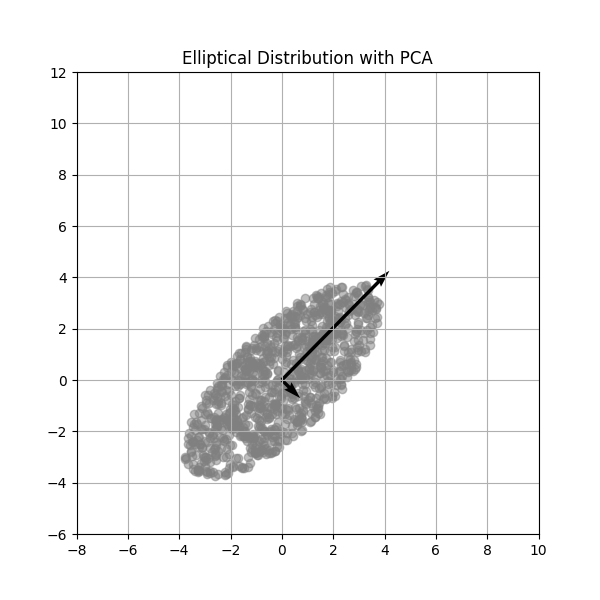
\includegraphics[width=0.8\linewidth]{assets/pca.png}
    \caption{PCA原理}
    \label{tag:pca}
\end{figure}

 (1) 数据中心化:首先,对原始数据进行中心化处理,即将每个特征减去该特征的均值,使数据的均值为零

 (2) 计算数据的协方差矩阵,它描述了各个特征之间的关系和方差。对于一个 \(n \times m\) 的数据矩阵 \(\mathbf{X}\),其协方差矩阵为:$\Sigma = \frac{1}{n-1} \mathbf{X}^T \mathbf{X}$


(3) 计算特征值和特征向量
通过对协方差矩阵 \(\Sigma\) 进行特征值分解,得到其特征值和特征向量。特征向量代表了数据中变化的方向,特征值表示该方向上的方差大小。计算得到的特征向量就是主成分的方向。


(4) 选择主成分,构成转换矩阵
选择特征值最大的几个特征向量作为主成分,这些主成分保留了数据中最大的方差。选择的特征向量数量决定了降维后的维度。通过将原始数据投影到选定的主成分上,得到降维后的数据。假设选取前 \(k\) 个特征向量作为主成分,则新的数据矩阵为:

\[
\mathbf{X}_{PCA} = \mathbf{X}_{centered} \cdot \mathbf{V}_k
\]
其中,\(\mathbf{V}_k\) 是由前 \(k\) 个特征向量组成的矩阵,\(\mathbf{X}_{PCA}\) 是降维后的数据矩阵。

将PCA技术应用到现有的基于高维特征概率密度估计的模型不确定性建模框架中,基本的流程如下。\textbf{在训练阶段},首先完成神经网络训练,之后在训练集上使用神经网络提取训练数据的高维特征。这些特征通常来自神经网络某一层的输出,代表输入数据的高维表示。之后对提取的高维特征进行主成分分析,计算特征协方差矩阵并对其进行特征分解,获取主成分方向。根据累计方差贡献率(如 95\% 或 99\%)选择前 k 个主成分,从高维空间降维到k维。使用 PCA 转换矩阵将原始高维训练特征投影到 k 维主成分空间,得到降维后的训练特征。在降维后的特征空间中,训练高斯判别分析模型,估计混合成分的均值、协方差矩阵和权重参数。训练完成后,保存 PCA 转换矩阵和 GDA 模型的参数。

\textbf{在不确定性计算阶段}。对测试数据通过同一神经网络提取高维特征,保证特征分布与训练阶段一致。使用训练阶段保存的 PCA 转换矩阵,将测试数据的高维特征投影到k 维主成分空间。注意:在此阶段,不需要计算 PCA 转换矩阵,而是必须使用训练阶段的转换矩阵以确保一致性。将降维后的测试特征输入到训练好的 GDA 模型中,计算每个数据点属于各个高斯分布成分的概率,同时直接输出分类结果(如最大后验概率对应的类别)。

总之,应用PCA降维到现有的算法上,主要分为训练阶段和不确定性计算阶段。训练阶段完成从高维特征提取、PCA建模到GDA参数估计的一系列操作,目的是学习特征空间的低维表示及其概率分布。不确定性计算阶段应用训练阶段学习到的 PCA 转换和 GDA 模型,对测试数据进行降维和分类推断。这种分阶段的操作流程能够保证训练和测试时的特征空间一致性,并大幅减少高维特征带来的计算复杂度和GDA模型的存储复杂度。



下面从理论上分析以下加入PCA降维后时间复杂度和空间复杂度的变化。已知多元高斯分布的概率密度函数为:

\[
p(\mathbf{z} \mid \boldsymbol{\mu_c}, \boldsymbol{\Sigma_c}) = \frac{1}{(2\pi)^{\frac{D}{2}} \left| \boldsymbol{\Sigma_c} \right|^{\frac{1}{2}}} \exp \left( -\frac{1}{2} (\mathbf{z} - \boldsymbol{\mu_c})^T \boldsymbol{\Sigma_c}^{-1} (\mathbf{z} - \boldsymbol{\mu_c}) \right)
\]
\textbf{在时间复杂度的方面},在高斯判别分析模型(GDA)中,假设已经完成了训练,因此均值向量和协方差矩阵已经预先计算好。假设特征向量的维度为 \( M \),对于每个类别 \( k \),计算一个特征向量的概率密度时,首先需要计算差 \( (\mathbf{z} - \mu_k) \),其时间复杂度为 \( O(M) \)。然后计算矩阵乘法 \( \Sigma_k^{-1} (\mathbf{z} - \mu_k) \),这一步的时间复杂度为 \( O(M^2) \),接着进行标量计算 \( (\mathbf{z} - \mu_k)^T \Sigma_k^{-1} (\mathbf{z} - \mu_k) \),其时间复杂度为 \( O(M) \)。此外,协方差矩阵的行列式和平方根计算已被忽略。由于这些步骤需要对每个特征向量进行计算,因此降维前的总时间复杂度为 \( O(M^2) \)。

当特征维度通过主成分分析(PCA)降到 \( N \) 维时,首先对原始特征向量进行降维。假设降维矩阵 \( P \) 已经预先计算好,降维操作的时间复杂度为 \( O(M \cdot N) \)。然后,对于降维后的 \( N \)-维特征向量,首先计算差 \( (\mathbf{z'} - \mu_k) \),其时间复杂度为 \( O(N) \),接着计算矩阵乘法 \( \Sigma_k^{-1} (\mathbf{z'} - \mu_k) \),这一步的时间复杂度为 \( O(N^2) \),最后进行标量计算 \( (\mathbf{z'} - \mu_k)^T \Sigma_k^{-1} (\mathbf{z'} - \mu_k) \),其时间复杂度为 \( O(N) \)。因此,降维后的时间复杂度为 \( O(M \cdot N + N^2) \),其中 \( O(M \cdot N) \) 是降维操作的复杂度,\( O(N^2) \) 是 GDA 计算的复杂度。

\textbf{在空间复杂度方面},降维前每个类别的均值向量 \( \mu_k \) 需要 \( O(M) \) 空间,协方差矩阵 \( \Sigma_k \) 需要 \( O(M^2) \) 空间。因此,对于 \( K \) 个类别,存储所有均值向量和协方差矩阵的总空间复杂度为 \( O(K \cdot M^2) \)。特征向量 \( \mathbf{x} \) 需要 \( O(M) \) 空间。降维后的均值向量 \( \mu_k \) 需要 \( O(N) \) 空间,协方差矩阵 \( \Sigma_k \) 需要 \( O(N^2) \) 空间。因此,对于 \( K \) 个类别,存储所有均值向量和协方差矩阵的空间复杂度为 \( O(K \cdot N^2) \),降维后的特征向量 \( \mathbf{z'} \) 需要 \( O(N) \) 空间,降维矩阵 \( P \) 需要 \( O(M \cdot N) \) 空间。综上,降维后的总空间复杂度为 \( O(K \cdot N^2 + M \cdot N) \),通常由于 \( N < M \),降维后空间复杂度显著低于降维前的空间复杂度。




基于辅助损失函数联合训练并使用PCA降维加速的改进算法流程图见\ref{alg:2}。


\begin{algorithm}[h]
	\caption{基于输入扰动的概率密度建模的模型不确定性算法}
	\label{alg:2}
	
	\begin{algorithmic}[1]
		\Require 训练集: $(X,Y)$ 
		\Require 高维特征提取网络: $f_{\theta}:x \rightarrow \mathbf{R}^d $ 
		\Require GDA模型: $q(z) = \max_{c}q(z|y=c)$
		
		\\
		\Procedure {1.训练阶段}{}
            \State 初始化类中心$C_i$
		\State 使用$CELoss+\lambda*AuxLoss$,在训练数据集数据集上训练网络$f_{\theta}$


		\EndProcedure
            \\
        
		\Procedure {2.PCA训练和GDA建模}{}
		\State 在训练集上抽取高维特征,并训练PCA模型$F_{proj}$
            \For {属于类别c的样本}
		\State $\mu_{c}=F_{proj}(\frac{1}{|x_c|}f_{\theta}(x_c))$
		\State $\Sigma_c = \frac{1}{|x_c|-1}(F_{proj}(f_{\theta}(x_c))-\mu_c)(F_{proj}(f_{\theta}(x_c))-      \mu_c)^T$
		\State q(y=c)=$\frac{|X_C|}{|X|}$
            \EndFor
		\EndProcedure 
            \\

        
		\Procedure {3.模型不确定性计算}{}
		\State $z=F_{proj}(f_{\theta}(x))$
		\State 计算模型不确定性 $Uncertainty(x) = \log \max_{c}q(z|y=c)$,其中$q(z|y=c)\sim N(\mu_c,\Sigma_c)$
		\EndProcedure 
	\end{algorithmic}
\end{algorithm}


\section{实验结果与分析}
为了评估本文所提出的基于辅助损失函数联合训练,对模型不确定性建模效果的提升,本节分别在OOD检测任务上,误分类样本识别等任务上进行了评估。本节的实验内容主要是在CIFAR-10,CIFAR-100,SVHN,MNIST,LSUN等数据集和VGG,ResNet,VIT等模型进行的。为了评估使用辅助损失函数联合训练对模型不确定建模效果的影响,本文评估单独使用交叉熵损失函数(CELoss)和辅助损失函数(AuxLoss)+交叉熵损失函数(CELoss)联合训练两种不同的训练策略得到的模型,在模型训练时,有关批次,批大小,优化器,初始学习率等超参数设置见下表格\ref{tab:模型训练2}。在训练的时候,针对网络权重参数和辅助损失函数里面的类中心参数,分别使用了两个不同的优化器,关于两个优化器超参数设置见表格\ref{tab:模型训练2}。
\begin{table}[htbp]
	\captionsetup{font=small, justification=centering}
	\centering
	\resizebox{\linewidth}{!}{
	\begin{tabular}{c c c c c c c c c c c}
	\hline
	模型结构 & 数据集 & 批次 & 批大小 & $\lambda$ & 优化器1 & 优化器2 & 优化器1学习率 & 优化器2学习率 & 动量 & 权重衰减 \\
	\hline
	VGG16 & CIFAR10 & 300 & 512 & 20 &SGD & SGD & 0.1  & 0.5 & 0.9 & 0.0005 \\
        ResNet50 & CIFAR10 & 300 & 512 & 20 &  SGD & SGD  & 0.1  & 0.5 & 0.9 & 0.0005 \\
        VIT & CIFAR10 & 300 & 512 &  20 &  SGD & SGD & 0.01  & 0.5 & 0.9 & 0.0005 \\
	\hline
	\end{tabular}
	}
	\caption{
	模型训练超参数设置
	}
        \label{tab:模型训练2}
\end{table}


\subsection{OOD检测任务上评估}

以上通过可视化特征空间,验证了所提出的新的辅助损失函数和交叉熵损失函数联合训练,能够提升特征空间上不同类别样本的类内紧密性和类间可分性。为了验证联合训练基于高维特征概率密度建模不确定性的影响,本节在OOD检测任务上评估使用辅助损失函数联合训练对模型不确定建模效果的影响,本节选择CIFAR10数据集的训练集,使用交叉熵损失函数(CELoss)单独训练VGG/ResNet50/VIT等不同模型,然后再使用辅助损失函数(AuxLoss)和交叉熵损失函数(CELoss)联合训练的策略训练VGG/ResNet50/VIT等不同模型。使用CIFAR10数据集的测试集作为分布内样本,SVHN、CIFAR100、LSUN、MNIST等数据集作为分布外样本,构建OOD检测任务,评估两种不同的训练策略对模型不确定性的建模效果,实验结果如表\ref{OOD}。


\begin{table}[h]
\captionsetup{font=small, justification=centering}
\centering
\renewcommand{\arraystretch}{1.2}
\setlength{\tabcolsep}{8pt}
\begin{tabular}{c c c c c}
\hline
\textbf{训练策略} & \textbf{OOD Dataset} & \textbf{VGG} & \textbf{ResNet} & \textbf{ViT} \\ 
\hline
\multirow{4}{*}{CE Loss} 
& SVHN & \textbf{0.9325}/0.9057 & 0.9179/0.9415 & 0.9779/0.9843 \\ 
& LSUN & \textbf{0.9160/0.9274} & 0.9239/0.9390 & 0.9906/0.9917 \\ 
& CIFAR100 & \textbf{0.8948/0.9054} & 0.8888/0.9018 & 0.9571/0.9605 \\ 
& MNIST & 0.9195/0.9225 & 0.9292/0.9511 & 0.9823/0.9854 \\ 
\midrule
\multirow{4}{*}{联合训练} 
& SVHN & 0.9247/\textbf{0.9459} &\textbf{ 0.9547/0.9655} & \textbf{0.9855/0.9893} \\ 
& LSUN & 0.9046/0.8858 & \textbf{0.9478/0.9462} & \textbf{0.9955/0.9963 }\\ 
& CIFAR100 & 0.8827/0.8805 &\textbf{ 0.9123/0.9129} & \textbf{0.9630/0.9648 }\\ 
& MNIST & \textbf{0.9304/0.9474} & \textbf{0.9631/0.9728} & \textbf{0.9893/0.9918} \\ 
\hline
\end{tabular}
\caption{OOD检测任务上评估,合并后的实验结果,显示不同训练策略和模型在多个 OOD 数据集上的表现。}
\label{OOD}
\end{table}


从表格\ref{OOD}结果可以看出,加入辅助损失函数的联合训练策略在各模型(VGG、ResNet、ViT)和多个数据集(SVHN、LSUN、CIFAR100、MNIST)的OOD检测任务上均显著提升了AUROC/AUPRC指标,这表明联合训练策略的引入有效增强了模型在 OOD 数据集上的检测能力,表现为更高的 AUROC 和 AUPR 分数。使用新提出的损失函数联合训练的策略在OOD检测任务上的效果提升,验证了在使用辅助损失函数联合训练的特征空间上进行概率分布的建模,能更好地建模神经网络的不确定性。

\subsection{误分类样本识别任务上评估}

误分类样本检测任务用于评估神经网络在预测结果上的不确定性,是通过模型能否依据不确定性值识别出预测错误的样本。本节在CIFAR10数据集的训练集上,使用交叉熵损失函数(CELoss)和辅助损失函数(AuxLoss)+交叉熵损失函数(CELoss)联合训练两种不同的训练策略训练VGG/ResNet50/VIT等不同模型,并在CIFAR10测试集进行误分类样本识别实验,实验结果如图\ref{tab:misclassified2}。

实验结果表明,加入辅助损失函数联合训练的改进方法在所有模型上均显著提升了 AUROC 和 AUPRC 指标,这表明加入辅助损失函数联合训练能够有效增强模型对误分类样本的检测能力,提高模型的不确定性建模能力。

同时本实验评估了加入辅助损失函数前后训练出的模型的校准性能,该性能由ECE指标表示,ECE指标越小说明模型校准能力越好。从表\ref{tab:misclassified}中可以看出,加入辅助损失函数联合训练的改进方法在所有模型上在ECE指标上均降低了,ECE指标越低表明模型的预测概率与实际准确率之间的匹配程度较好,即模型是校准良好的,由此得出结论:辅助损失函数联合训练的改进方法能够提高模型的校准性能。
\begin{table}[h]
    \captionsetup{font=small, justification=centering}
    \centering
    \renewcommand{\arraystretch}{1.0} % Adjust line spacing
    \resizebox{\linewidth}{!}{
    \begin{tabular}{l l c c c}
    \toprule
    Method & Model & AUROC($\uparrow$) & AUPRC($\uparrow$) & ECE($\downarrow$) \\
    \midrule
    \multirow{5}{*}{\vspace{4em} CELoss} 
    & VGG16 & 0.9274  & 0.9945 & 0.0404\\
    & ResNet50 &  0.9344 & 0.9963 & 0.0286 \\
    & VIT & 0.9481 & 0.9984 &0.0167 \\
    \midrule
    \multirow{5}{*}{\vspace{4em} 联合训练} 
    & VGG15 & \textbf{0.9343} & \textbf{0.9951} & \textbf{0.0401} \\
    & ResNet50 & \textbf{0.9450}  & \textbf{0.9969} &\textbf{0.0344}\\
    & VIT & \textbf{0.9479}  & \textbf{0.9980} &\textbf{0.0166}\\
    \bottomrule
    \end{tabular}
    }
    \caption{误分类样本检测任务,实验结果在不同的模型(VGG16、ResNet50、VIT)上做实验,对比交叉熵损失函数训练和使用辅助损失函数联合训练对模型不确定性的建模效果,报告指标是AUROC($\uparrow$) / AUPRC($\uparrow$)/ECE($\downarrow$)}
    \label{tab:misclassified2}
\end{table}


\subsection{PCA降维对模型不确定性的影响}

高维特征概率密度建模面临维度灾难、计算复杂度和过拟合风险等挑战,为解决这些问题,本文采用PCA降维技术来减少特征空间的复杂性,提升建模效果。本节实验探究PCA算法降维前后,在OOD检测任务上模型不确定性的表现,算法实现使用sklearn.decomposition.PCA,该实现中最重要的参数是n\_components,表示降维后的保留特征的维度大小。在 sklearn.decomposition.PCA 中,n\_components参数用于控制PCA算法选择的主成分数量,具体设置方式如下:

\begin{enumerate}
  \item \textbf{整数值} ($n\_components = k$):
    如果 $n\_components$ 设置为一个整数 $k$,则PCA会选择保留前 $k$ 个主成分,$k$ 需要小于或等于输入数据的特征数 。这样做会将数据降维到 $k$ 个维度。

  \item \textbf{浮点数} ($0 < n\_components < 1$):
    如果 $n\_components$ 设置为介于0和1之间的浮动值(如0.95),PCA将选择最小的主成分数,以保证这些主成分解释的数据方差比例大于该浮动值。
  \item \textbf{'mle'} :
    如果 $n\_components$ 设置为 'mle',PCA会使用Minka的MLE方法自动选择最合适的主成分数。该方法通过估计数据的协方差矩阵的最大似然估计来决定主成分的数量。


\end{enumerate}

实验中在CIAFR10数据集上训练了不同的模型(VGG16、ResNet50、VIT),PCA算法设置n\_components采用网格搜索的方法,从128到最到维度按照间隔32搜索最合适的维度。在训练数据集的特征上训练PCA模型,然后在OOD检测任务上评估加入PCA降维前后模型的不确定性建模效果。实验结果见表\ref{tab:PCA_results_CIFAR10}
\begin{table}[h]
    \captionsetup{font=small, justification=centering}
    \centering
    \renewcommand{\arraystretch}{1.0} % Adjust line spacing
    \resizebox{\linewidth}{!}{
    \begin{tabular}{l l c c c}
    \toprule
    Method & OOD Dataset & VGG16+CIFAR10 & ResNet50+CIFAR10 & VIT+CIFAR10 \\
    &  & (Accuracy=0.9405) & (Accuracy=0.9489) & (Accuracy=0.9658) \\
    \midrule
    \multirow{4}{*}{联合训练} 
    & SVHN & 0.9190 / \textbf{0.9423} & 0.9102 / 0.9374 & 0.9835 / 0.9872 \\
    & LSUN & 0.9055 / 0.9255 & 0.9365 / 0.9232 & 0.9888 / 0.9906 \\
    & CIFAR100 & 0.8838 / 0.8972 & \textbf{0.9068} / 0.8883 & 0.9566/ 0.9588 \\
    & MNIST & 0.9206 / 0.9405 & 0.9005 / 0.9305 & 0.9849 / 0.9870 \\
    \midrule
    \multirow{4}{*}{联合训练+PCA} 
    & SVHN & \textbf{0.9200} / 0.9419 & \textbf{0.9197} / \textbf{0.9413} & \textbf{0.9846} / \textbf{0.9879} \\
    & LSUN & \textbf{0.9197} / \textbf{0.9343} & \textbf{0.9365} / \textbf{0.9455} & \textbf{0.9898} / \textbf{0.9914} \\
    & CIFAR100 & \textbf{0.8910} /\textbf{ 0.9030} & 0.9031 / \textbf{0.9137} & \textbf{0.9571} / \textbf{0.9580} \\
    & MNIST & \textbf{0.9304} / \textbf{0.9465} & \textbf{0.9282} / \textbf{0.9957} & \textbf{0.9858} / \textbf{0.9879} \\
    \bottomrule
    \end{tabular}
    }
    \caption{数据集选择CIFAR10,在不同的模型(VGG16,ResNet50,VIT)上做训练,对比联合训练和联合训练+PCA降维对模型不确定性的建模效果,报告指标是AUROC($\uparrow$) / AUPRC($\uparrow$)}
    \label{tab:PCA_results_CIFAR10}
\end{table}

加入PCA降维后,在一些模型和数据集上的AUROC和AUPRC指标显著提高。这表明,PCA能够帮助降低高维数据的噪声,在低维空间上更容易建模分布,减弱高维空间上存在的稀疏性和维度灾难等问题,进而提高OOD检测的性能。对于VGG16这样相对简单的模型,PCA的提升效果较小,因为VGG16本身提取的高维特征512维相对较低。分析降维后有些数据集上OOD检测能力提升,可能的原因时模型能够更加聚焦于关键特征,减少冗余信息的干扰,从而提高不确定性建模和OOD检测的效果。



\subsubsection{PCA与维度的分析}

PCA降维中维度大小对结果有很大的影响,本节实验还探讨了模型不确定性建模效果与PCA降维特征维度的关系。实验中在CIFAR10数据集上训练ResNet50模型,对于训练数据抽取的特征使用PCA降维,设置n\_components参数为整数并使用网格搜索遍历[256,512,1024]等不同维度,统计降维前后在OOD检测任务上的时间、存储、以及AUROC/AUPRC指标,实验结果见\ref{fig:PCA-dimension}

\begin{figure}[h]
    \captionsetup{font=small, justification=centering}
    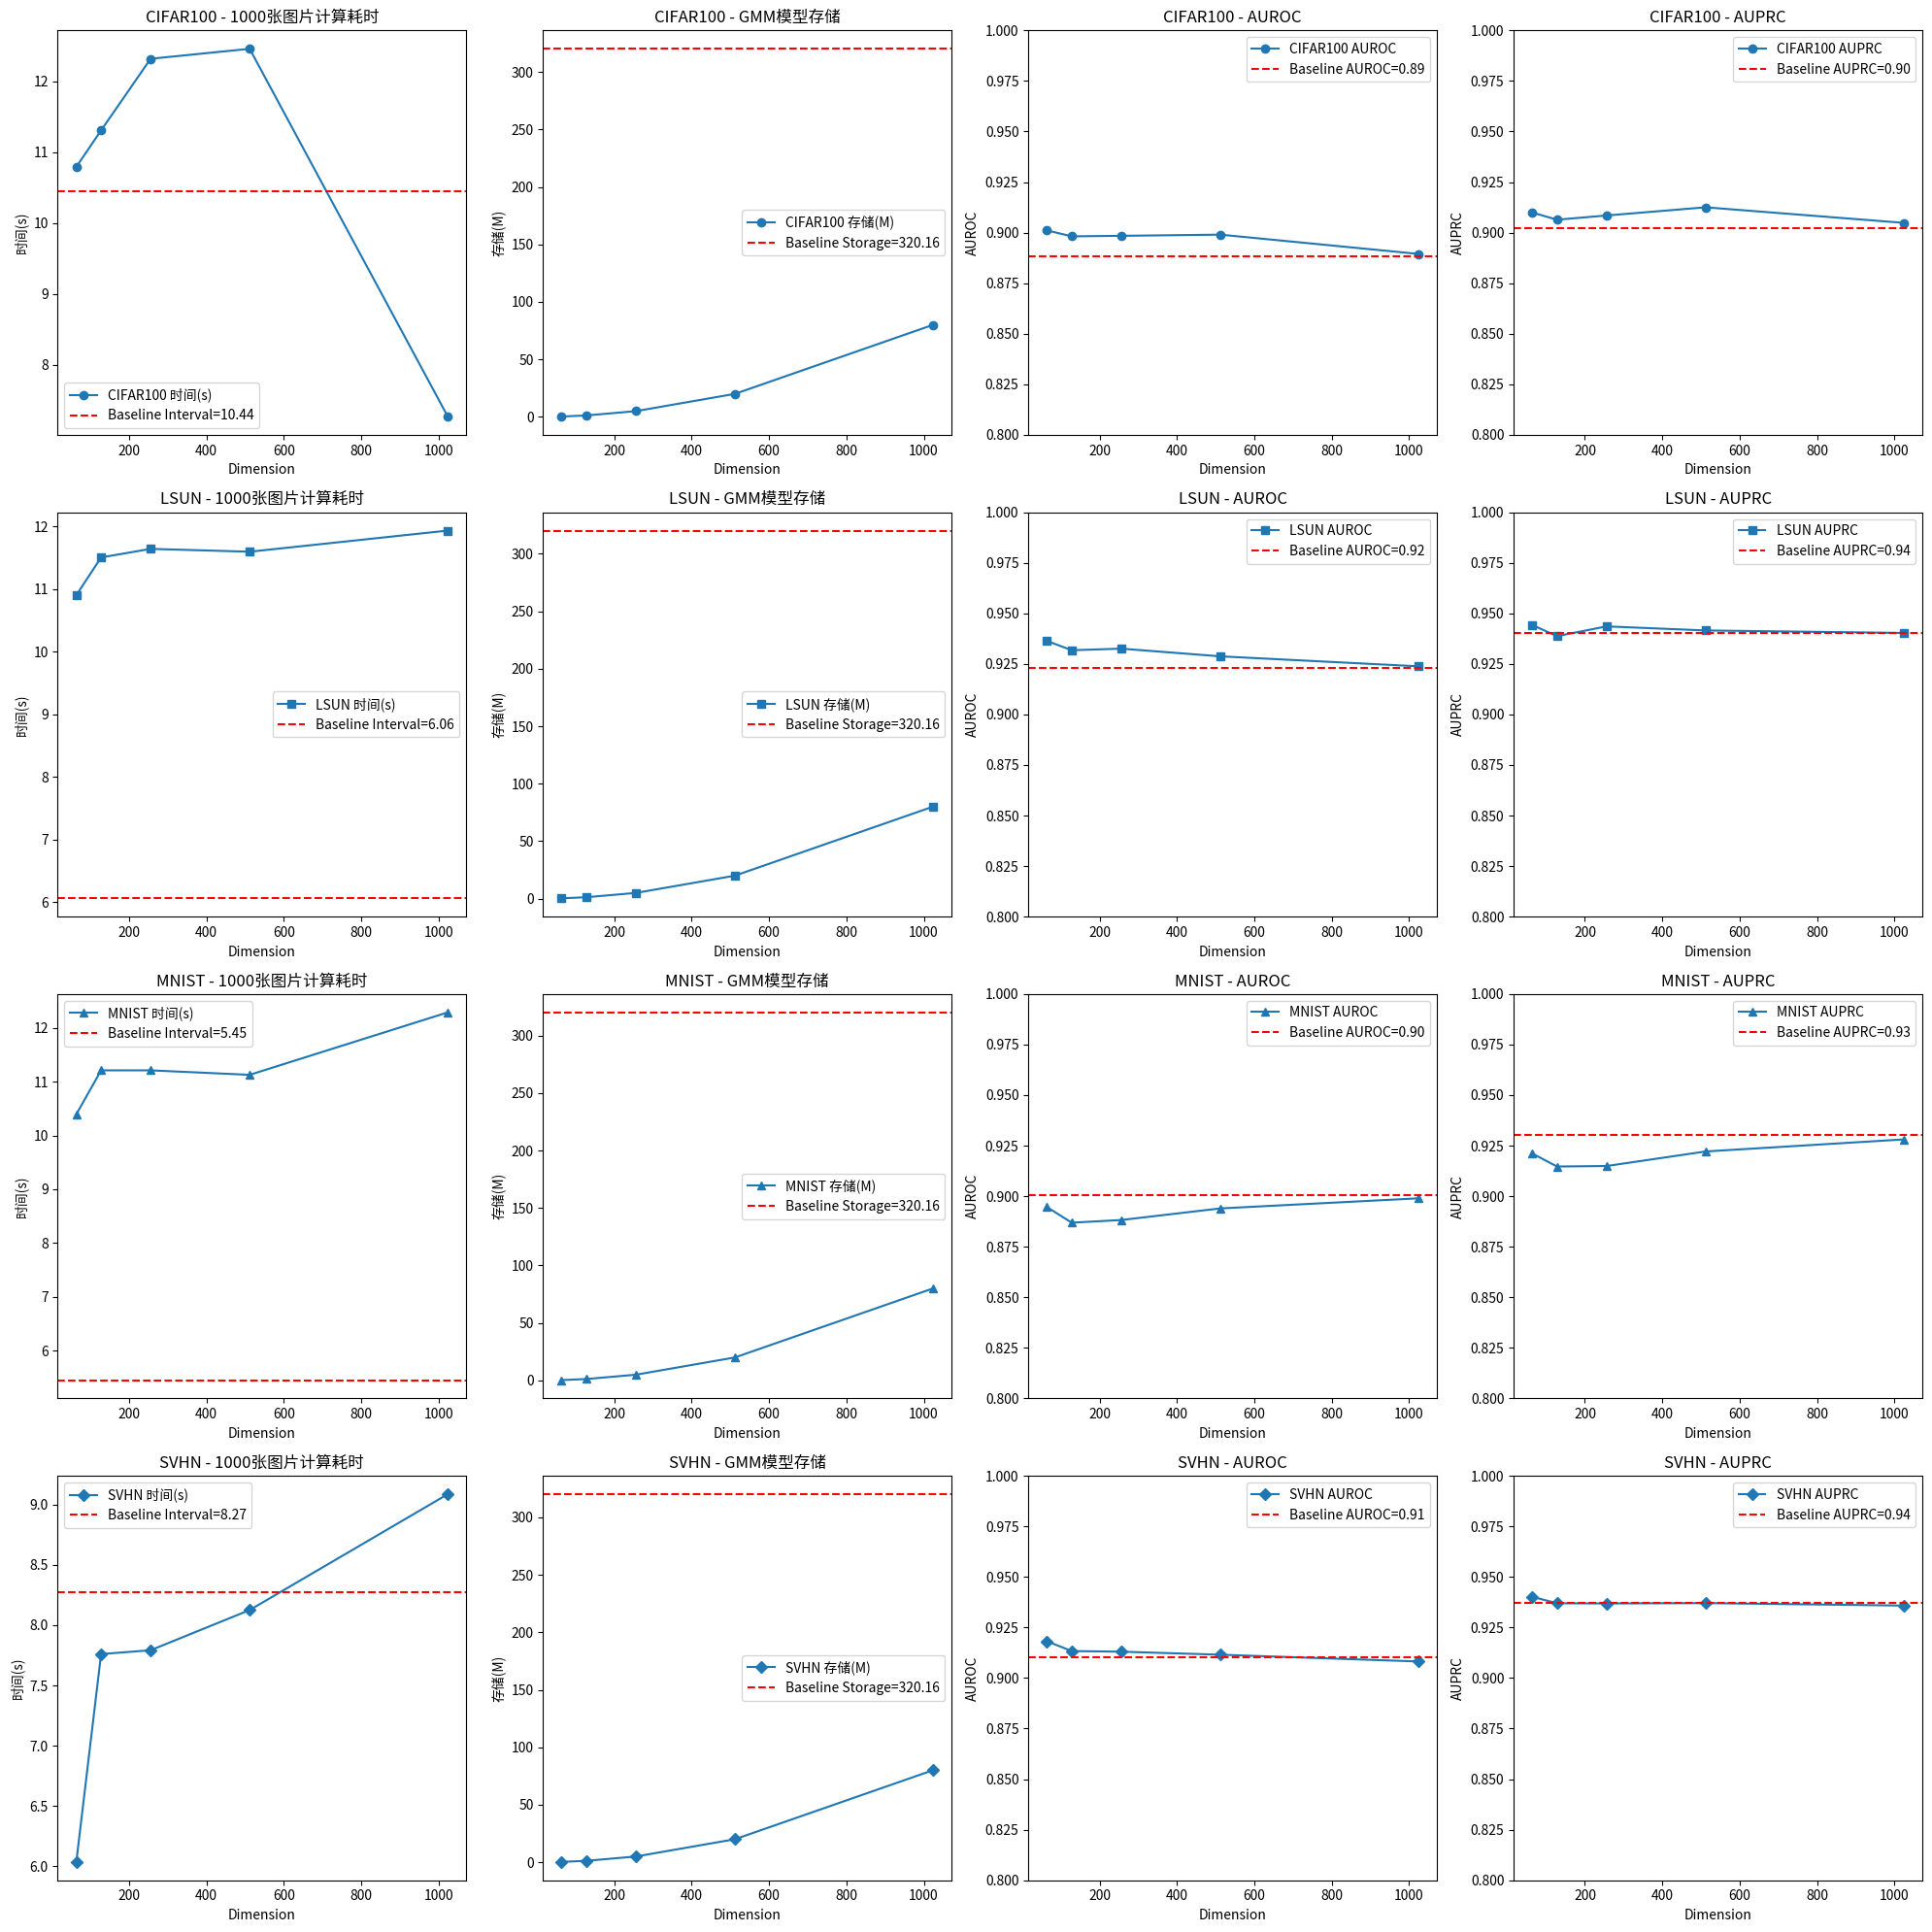
\includegraphics[width=1.\linewidth]{assets/pca_plots_dimension.png}
    \caption{PCA维度的分析,红色基线是未降维时的结果,蓝色线是在不同维度下的不同指标随降维维度的变化趋势}
    \label{fig:PCA-dimension}
\end{figure}

从图\ref{fig:PCA-dimension}中可以看出,实验在 CIFAR-100、LSUN、MNIST 和 SVHN 四个数据集上分析了 PCA 降维在不同维度(256 至 1024 维)下对计算时间、存储需求以及对模型不确定性建模效果(通过OOD检测任务上的AUROC 和 AUPRC指标反映)的影响。结果表明,计算时间随着维度的增加显著增长,高维度情况下的计算开销尤为明显,同时整体上看降维后的计算耗时都高于基线,这与上面降维后时间复杂度降低的理论分析相矛盾,这是因为在实验中PCA算法是使用sklearn中的实现,计算是在CPU上进行的,降维后的计算时间一部分在CPU计算,一部分在GPU上计算,相比降维前全都在GPU上运算,可能会出现降维后计算时间反而变大。高斯判别分析模型的参数均值和协方差矩阵的存储需求也随着维度增长,且在所有的维度上,降维后存储开销显著低于基线模型,展现出良好的存储效率,且存储随着维度的变化接近指数增长,与前文的理论分析一致。与此同时,AUROC 和 AUPRC 两项性能指标在各数据集上的没有因为降维大幅度减少,即使在较低维度(如 256 维)情况下,对不确定性的建模效果几乎未受到影响,说明 PCA 能够在显著降低数据规模的同时很好地保留数据的关键信息,在某些数据集上AUROC/AUPRC降维后甚至会升高,这可能是因为在降维后减弱了高维情况下可能出现的维度灾难。

综合以上分析为了降低计算开销,建议在实际应用中结合计算资源限制选择较低的降维维度(如 256-512 维)。综合存储需求、计算时间和性能指标的变化,选择 256-512 维 是较为合理的范围,可以在存储和性能之间取得最佳平衡。

\subsection{消融实验}
在这节实验中,通过消融实验,对比提出的方法的有效性,主要观察加入辅助损失函数联合训练和加入输入扰动对模型不确定性建模效果的影响。在联合训练的基础上,本节结合第三章提出的基于输入扰动的改进,在OOD检测任务上评估对模型不确定性建模效果。
实验中首先在CIFAR10数据集上进行VGG16/ResNet50/VIT等模型的训练,训练完成后选取SVHN/LSUN/CIFAR100/MNIST等数据集作为域外样本进行OOD检测任务的评估。实验结果见表\ref{tab:combined_3_4}



\begin{table}[h]
	\captionsetup{font=small, justification=centering}
	\centering
	\renewcommand{\arraystretch}{1.0} % Adjust line spacing
	\resizebox{\linewidth}{!}{
            \begin{tabular}{l l c c c}
            \toprule
            Method & OOD Dataset & VGG16+CIFAR10 & ResNet50+CIFAR10 & VIT+CIFAR10 \\
            &  & (Accuracy=0.9405) & (Accuracy=0.9489) & (Accuracy=0.9600) \\
            \midrule
            \multirow{4}{*}{CE} 
            & SVHN & \textbf{0.9325}/0.9057 & 0.9179/0.9415 & 0.9779/0.9843 \\ 
            & LSUN & \textbf{0.9160/0.9274} & 0.9239/0.9390 & 0.9906/0.9917 \\ 
            & CIFAR100 & \textbf{0.8948/0.9054} & 0.8888/0.9018 & 0.9571/0.9605 \\ 
            & MNIST & 0.9195/0.9225 & 0.9292/0.9511 & 0.9823/0.9854 \\ 
            \midrule
            \multirow{4}{*}{联合训练} 
            & SVHN & 0.9247/\textbf{0.9459} & 0.9547/0.9655 & 0.9855/0.9893 \\ 
            & LSUN & 0.9046/0.8858 & \textbf{0.9478/0.9462} & 0.9955/0.9963 \\ 
            & CIFAR100 & 0.8827/0.8805 & 0.9123/0.9129 & \textbf{0.9630/0.9648 }\\ 
            & MNIST & 0.9304/0.9474 & 0.9631/0.9728 & 0.9893/0.9918 \\ 
            \midrule
            \multirow{4}{*}{联合训练+输入扰动} 
            & SVHN & 0.9234/0.9440 &\textbf{ 0.9724/0.9778} & \textbf{0.9868/0.9906} \\
            & LSUN & 0.9018/0.8821 & 0.9462/0.9407 & \textbf{0.9994/0.9994} \\
            & CIFAR100 & 0.8826/0.8801 & \textbf{0.9318/0.9173 }& 0.9629/0.9635 \\
            & MNIST  & \textbf{ 0.9571/0.9636 }&\textbf{ 0.9723/0.9794} &\textbf{ 0.9960/0.9962} \\
            \bottomrule
		\end{tabular}
	}
	\caption{在CIFAR10数据集上训练VGG/ResNet50/VIT等模型,选取SVHN、CIFAR100、MNIST、LSUN等数据集作OOD数据集,在OOD检测任务上做实验对比CrossEntropy训练、CrossEntropy+AuxLoss联合训练、联合训练+输入扰动对模型不确定性的建模效果,报告指标是AUROC($\uparrow$) / AUPRC($\uparrow$),越高越好}
	\label{tab:combined_3_4}
\end{table}


表格\ref{tab:combined_3_4}中的实验结果展示了在不同模型(VGG16、ResNet50、VIT)上对四个OOD数据集(SVHN、LSUN、CIFAR100、MNIST)的OOD检测性能的影响,评估了三种方法(CrossEntropy、CrossEntropy+AuxLoss联合训练、联合训练+输入扰动)对模型不确定性的建模效果。从OOD检测结果来看,加入辅助损失函数联合训练结合输入扰动的方法在相比于另外两种单纯使用交叉熵损失训练和仅联合训练的方法,在所有模型和数据集上均显著提升了检测性能,这表明辅助损失函数联合训练的方法增强了模型对模型不确定性的捕捉能力,而输入扰动进一步提高了对不确定性的建模能力。加入AuxLoss的联合训练策略在增强模型对类间分布的区分能力方面表现出显著优势,而引入输入扰动进一步提高了模型在复杂分布下不确定性建模的鲁棒性和泛化能力。

\section{本章小结}
为了进一步提升基于高维特征概率密度估计的不确定性建模效果,本章提出使用辅助损失函数联合训练来优化特征空间表示的方法。神经网络的分类性能和不确定性建模效果直接依赖于特征空间的结构。理想的特征空间应具备较高的类内样本紧密性和类间可分性,这有助于模型更好地区分不同类别,提升模型的稳定性和鲁棒性。然而,在实际应用中,神经网络通常难以同时优化这两个方面,导致特征空间分布混乱,进而影响模型表现。度量学习可以通过学习一个合适的距离度量来优化特征空间表示,使得同一类别的样本尽可能紧密,而不同类别的样本保持较大间距,从而改善模型的分类性能。

本章基于度量学习提出了一种新的辅助损失函数AuxLoss,AuxLoss在传统CenterLoss的基础上引入了类别中心间距的约束,不仅加强了类内样本的紧密性,还优化了类间的可分性。通过t-SNE可视化高维特征空间,可以看到使用AuxLoss联合训练后的模型在高维特征空间上展现出更加清晰的类别边界,类别间的分隔更加明显,能够进一步提升了模型的分类稳定性和鲁棒性。使用Davies-Bouldin指数和Fisher比率等指标定量评估类内紧密性和类间可分性,结果也显示使用AuxLoss联合训练能够带来明显的提升,从而增强了模型对不确定性的捕捉能力。本章实验部分,在OOD检测和误分类样本识别等任务上评估对不确定性的建模效果,结果表明,采用辅助损失函数联合训练的模型在不确定性建模上表现出明显的优势。

此外,本章还探讨了如何结合PCA降维来应对高维数据建模中的计算复杂性和存储复杂性问题。PCA能够有效降低数据的维度,同时保留主要方差,减少计算开销和存储空间。实验结果表明,PCA降维技术在减少存储开销的同时,依然能够保持或提升模型在不确定性上的建模能力。

总体而言,本章提出的特征空间优化方法,通过结合度量学习、AuxLoss损失函数以及PCA降维,显著提高了神经网络的分类精度和不确定性量化能力。这些研究不仅推动了神经网络不确定性建模的理论发展,也为实际应用中的异常检测、风险评估等任务提供了有力支持。未来的研究将着重于进一步优化特征空间结构,并探索更高效的不确定性量化方法。
\chapter{总结与展望}
\section{总结}
论文内容

\section{对神经网络不确定性研究的展望}

随着深度学习的广泛应用,神经网络的不确定性研究在模型安全性、鲁棒性和可靠性等领域展现出重要价值。以下是对未来研究方向的展望。

\subsection{更高效的不确定性建模方法}
现有的不确定性建模方法,如贝叶斯神经网络和深度集成方法,往往面临计算成本高和难以扩展的问题。未来研究可以关注以下方面:
\begin{itemize}
    \item \textbf{轻量化模型}:开发计算效率更高的模型,适用于大规模数据集和实时应用。
    \item \textbf{近似推断改进}:优化如变分推断和采样方法的效率,减小近似误差。
    \item \textbf{统一框架}:构建能够同时捕获数据不确定性和模型不确定性的统一建模框架。
\end{itemize}

\subsection{更可靠的评估标准}
当前对不确定性模型的评估依赖于间接任务(如 OOD 检测),难以全面反映实际性能。未来可以探索:
\begin{itemize}
    \item \textbf{真实任务驱动评估}:设计更加贴近实际应用的不确定性评估任务。
    \item \textbf{多维度评价体系}:结合模型性能(如准确率)、不确定性分布的合理性和计算效率,建立综合评估体系。
    \item \textbf{领域适配性分析}:研究不确定性模型在不同领域(如医学诊断、自动驾驶)的适配性。
\end{itemize}

\subsection{不确定性与因果推断结合}
不确定性建模和因果推断具有天然联系,未来研究可探索二者的结合:
\begin{itemize}
    \item \textbf{因果结构建模}:通过引入因果图或结构化知识,提升不确定性建模的解释性和可控性。
    \item \textbf{干预式不确定性分析}:研究在不同干预条件下模型预测不确定性的变化,为决策系统提供可靠支持。
\end{itemize}

\subsection{不确定性在复杂场景下的应用}
随着任务复杂度增加,不确定性建模需要适配新的应用场景,例如:
\begin{itemize}
    \item \textbf{多模态数据}:探索图像、文本和音频等多模态数据的不确定性建模方法。
    \item \textbf{在线学习与自适应系统}:开发能动态调整不确定性的模型,适应在线学习和环境变化。
    \item \textbf{社会与伦理影响}:研究不确定性模型在公平性、隐私保护和社会影响方面的作用。
\end{itemize}

\subsection{不确定性与大规模预训练模型结合}
近年来,大规模预训练模型(如 Transformer 和 GPT)在多个领域取得显著进展。不确定性研究未来可以聚焦于:
\begin{itemize}
    \item \textbf{预训练与微调阶段的不确定性}:研究大规模模型在不同训练阶段中的不确定性特性。
    \item \textbf{高效的不确定性标定}:开发针对大规模模型的不确定性标定方法。
    \item \textbf{泛化与迁移能力}:分析大规模预训练模型在迁移学习和跨领域任务中的不确定性。
\end{itemize}

\subsection{不确定性与人机协作系统}
在许多实际场景下,人类需要与 AI 系统协作完成复杂任务。不确定性可以作为协作中的重要信息:
\begin{itemize}
    \item \textbf{人机决策协同}:利用不确定性信息提高人类和模型联合决策的效率与可靠性。
    \item \textbf{交互式学习}:通过不确定性反馈指导用户与模型的交互,提升模型性能。
    \item \textbf{解释性与透明性}:通过不确定性量化增强系统的可解释性,使用户更信任 AI 系统。
\end{itemize}

神经网络不确定性研究作为机器学习的重要方向,未来将进一步推动 AI 系统的可靠性与广泛应用。随着理论方法的深入发展和新兴应用场景的拓展,不确定性建模将成为构建智能、透明和可信 AI 系统的核心技术之一。






% 附录部分
\appendix
一些额外实验


\chapter{公式推导}
一些公式


% 后置部分包含参考文献、声明页(自动生成)等
\backmatter

% 打印参考文献列表
\printbibliography

\begin{acknowledgements}
  致谢内容
\end{acknowledgements}

\end{document}
